\documentclass[12pt, a4paper]{report}

% --- Packages ---
\usepackage[utf8]{inputenc}
\usepackage[T1]{fontenc}
\usepackage[french]{babel}
\usepackage{graphicx}
\usepackage{booktabs}
\usepackage{amsmath}
\usepackage{geometry}
\usepackage{array}
\usepackage{enumitem}
\usepackage{hyperref}
\usepackage{xcolor}
\usepackage{titlesec}
\usepackage{lmodern}
\usepackage{microtype}
\usepackage{fancyhdr}
\usepackage{listings}
\usepackage{float}
\usepackage[scaled=0.85]{beramono}
\usepackage{tikz}
\usepackage{afterpage}
\usepackage{tcolorbox}
\usepackage{titletoc}
\usepackage{pdfpages}
\usepackage{marvosym}

% --- Font Configuration ---

% --- Color Definitions ---
\definecolor{primary}{RGB}{0,102,204}
\definecolor{secondary}{RGB}{102,102,153}
\definecolor{accent}{RGB}{204,0,0}
\definecolor{darkgray}{RGB}{90,90,90}
\definecolor{lightgray}{RGB}{240,240,240}
\definecolor{codegray}{rgb}{0.5,0.5,0.5}
\definecolor{codepurple}{rgb}{0.58,0,0.82}
\definecolor{codeblue}{rgb}{0,0,0.9}
\definecolor{codegreen}{rgb}{0.1,0.6,0.1}

% --- Page Geometry ---
\geometry{
  a4paper,
  left=2.5cm,
  right=2.5cm,
  top=2.5cm,
  bottom=2.5cm,
  headheight=15pt
}

% --- Header/Footer Setup ---
\pagestyle{fancy}
\fancyhf{}
\fancyhead[L]{\small Rapport de Stage}
\fancyhead[R]{\small Zakaria el Khaldi}
\fancyfoot[C]{\thepage}
\renewcommand{\headrulewidth}{0.4pt}
\renewcommand{\footrulewidth}{0.4pt}

% --- Title Formatting ---
\titleformat{\chapter}
  {\normalfont\LARGE\bfseries\color{primary}}
  {\thechapter}{1em}{}
\titlespacing*{\chapter}{0pt}{50pt}{40pt}

\titleformat{\section}
  {\normalfont\Large\bfseries\color{primary}}
  {\thesection}{1em}{}
\titleformat{\subsection}
  {\normalfont\large\bfseries\color{secondary}}
  {\thesubsection}{1em}{}
\titleformat{\subsubsection}
  {\normalfont\normalsize\bfseries\color{accent}}
  {\thesubsubsection}{1em}{}

% --- List Formatting ---
\setlist[itemize]{leftmargin=*, nosep}
\setlist[enumerate]{leftmargin=*, nosep}

% --- Hyperlink Setup ---
\hypersetup{
  colorlinks=true,
  linkcolor=primary,
  urlcolor=secondary,
  citecolor=accent
}

% --- Listings Setup for Code ---
\lstdefinestyle{codestyle}{
    basicstyle=\ttfamily\footnotesize,
    numbers=left,
    numberstyle=\tiny\color{codegray},
    stepnumber=1,
    numbersep=5pt,
    backgroundcolor=\color{white!95!black},
    showspaces=false,
    showstringspaces=false,
    showtabs=false,
    frame=tb,
    framextopmargin=3pt,
    framexbottommargin=3pt,
    rulecolor=\color{black!30!white},
    tabsize=2,
    captionpos=b,
    breaklines=true,
    breakatwhitespace=false,
    stringstyle=\color{codepurple},
    commentstyle=\color{codegreen},
    keywordstyle=\color{codeblue}
}

% Define JavaScript language for listings
\lstdefinelanguage{JavaScript}{
  keywords={break, case, catch, continue, debugger, default, delete, do, else, false, finally, for, function, if, in, instanceof, new, null, return, switch, this, throw, true, try, typeof, var, void, while, with, let, const, class, export, import, await, async},
  sensitive=true,
  comment=[l]{//},
  morecomment=[s]{/*}{*/},
  morestring=[b]',
  morestring=[b]"
}

% --- Image path configuration ---
\graphicspath{{pfe-pics/}}

% --- Document Information ---
\title{\Huge\bfseries\color{primary} Rapport de Projet de Fin d'Études \\ 
       \Large Développement d'un Système de Gestion Scolaire et d'une Plateforme de Création de Profils IA}
\author{\Large Zakaria el Khaldi}
\date{\large Juin 2025}

% --- TOC Formatting ---
\renewcommand{\contentsname}{Sommaire}

% Set up counter for tracking chapters and section numbering
\newcounter{mychapter}
\setcounter{mychapter}{0}

% Fix section numbering to use simple 1, 1.1 format with proper resetting
\makeatletter
\@addtoreset{section}{chapter}
\renewcommand{\thesection}{\arabic{section}}
\renewcommand{\thesubsection}{\thesection.\arabic{subsection}}
\renewcommand{\thesubsubsection}{\thesubsection.\arabic{subsubsection}}
\makeatother

% New TOC formatting
\titlecontents{chapter}
    [0em]                                       % left margin
    {\vspace{1.5em}\large\bfseries}             % above code (font size, weight)
    {\color{primary}}                           % numbered entry format (removed number)
    {\color{primary}}                           % unnumbered entry format
    {\titlerule*[1pc]{.}\contentspage}          % filler and page number
    [\vspace{0.5em}]                            % below code

% Format for section entries
\titlecontents{section}
    [2.3em]                               % left margin
    {\normalfont}                         % above code
    {\contentslabel{2.3em}}              % numbered entry format
    {}                                    % unnumbered entry format
    {\titlerule*[1pc]{.}\contentspage}    % filler and page number

% Format for subsection entries
\titlecontents{subsection}
    [4.6em]                               % left margin
    {\small}                              % above code
    {\contentslabel{2.8em}}              % numbered entry format
    {}                                    % unnumbered entry format
    {\titlerule*[1pc]{.}\contentspage}    % filler and page number

% Format for subsubsection entries
\titlecontents{subsubsection}
    [7.4em]                               % left margin
    {\small\itshape}                      % above code
    {\contentslabel{3.3em}}              % numbered entry format
    {}                                    % unnumbered entry format
    {\titlerule*[1pc]{.}\contentspage}    % filler and page number

% --- Chapter Styling ---
\def\@makechapterhead#1{%
  \vspace*{50\p@}%
  {\parindent \z@ \raggedright \normalfont
    \ifnum \c@secnumdepth >\m@ne
      \if@mainmatter
        \huge\bfseries\color{primary} #1
        \par\nobreak
        \vskip 20\p@
      \fi
    \fi
    \interlinepenalty\@M
    \ifnum \c@secnumdepth >\m@ne
      \if@mainmatter
      \else
        \Huge \bfseries \color{primary} #1
      \fi
    \else
      \Huge \bfseries \color{primary} #1
    \fi
    \par\nobreak
    \vskip 40\p@
    \hrule
    \vskip 40\p@
  }
  \newpage
}

\def\@makeschapterhead#1{%
  \vspace*{50\p@}%
  {\parindent \z@ \raggedright
    \normalfont
    \interlinepenalty\@M
    \Huge \bfseries \color{primary} #1\par\nobreak
    \vskip 40\p@
    \hrule
    \vskip 40\p@
  }
  \newpage
}

% --- Apply fancy style to all chapters automatically ---
\makeatletter
\renewcommand\chapter{\if@openright\cleardoublepage\else\clearpage\fi
                    \thispagestyle{fancy}%
                    \global\@topnum\z@
                    \@afterindentfalse
                    \secdef\@chapter\@schapter}
\makeatother

% --- Prevent duplicate chapter numbers ---
\renewcommand{\thechapter}{\arabic{chapter}}
\makeatletter
\renewcommand{\@seccntformat}[1]{%
  \ifcsname format#1\endcsname
    \csname format#1\endcsname
  \else
    \csname the#1\endcsname\quad
  \fi
}
\makeatother

% Format chapter numbering (hide in document text since it's in the title)
\makeatletter
\newcommand{\formatchapter}{}
\makeatother

\begin{document}

% --- Cover Page ---

\includepdf[pages=1]{page_de_garde_memoire.pdf}

% --- Preliminary Pages ---
% Add a generic label for all preliminary pages in TOC
\phantomsection
\addcontentsline{toc}{part}{Parties préliminaires}

% --- Dédicace ---
\chapter*{Dédicace}
\thispagestyle{fancy}

\begin{center}
\vspace*{2cm}
\textit{Je dédie ce modeste travail :}

\vspace{1cm}
\textit{À mes chers parents pour leur amour inconditionnel, leurs sacrifices et leur soutien constant tout au long de mon parcours.}

\vspace{0.5cm}
\textit{À ma famille et mes amis qui m'ont toujours encouragé et motivé.}

\vspace{0.5cm}
\textit{À tous mes professeurs qui ont contribué à ma formation et m'ont transmis leur savoir.}

\vspace{0.5cm}
\textit{À tous ceux qui croient en moi.}
\end{center}

\newpage

% --- Remerciements ---
\chapter*{Remerciements}
\thispagestyle{fancy}

\begin{center}
\vspace*{1cm}
\end{center}

Je tiens à exprimer ma profonde gratitude à toutes les personnes qui ont contribué à la réussite de ce projet de fin d'études et à l'élaboration de ce rapport.

Mes sincères remerciements s'adressent tout d'abord à mon encadrant, Pr. Ayman Naim, pour son accueil, sa disponibilité, son suivi régulier et ses précieux conseils qui m'ont guidé tout au long de cette expérience professionnelle.

Je souhaite également remercier l'ensemble de l'équipe pour leur accueil chaleureux, leur soutien et leur partage de connaissances qui ont rendu cette expérience particulièrement enrichissante.

Ma reconnaissance s'adresse aussi à l'administration et au corps professoral, pour la qualité de la formation dispensée dans la filière Développement des Systèmes d'Information, qui m'a fourni les compétences nécessaires pour mener à bien ce projet.

Je remercie particulièrement les professeurs qui ont contribué à ma formation et qui m'ont transmis les connaissances indispensables à la réalisation de ce travail.

Enfin, je tiens à exprimer ma gratitude envers ma famille et mes amis pour leur soutien moral, leurs encouragements constants et leur compréhension tout au long de mes études et durant la réalisation de ce projet.

\newpage

% --- Résumé ---
\chapter*{Résumé}
\thispagestyle{fancy}

Ce rapport présente les travaux réalisés durant mon projet de fin d'études, qui a consisté en la conception et le développement de deux systèmes complémentaires : un système de gestion scolaire complet et une plateforme de création de profils IA.

Le système de gestion scolaire est une solution multiplateforme (web et mobile) permettant aux établissements éducatifs de gérer efficacement les étudiants, les enseignants, les cours, les présences et les évaluations. Il offre des interfaces adaptées à chaque type d'utilisateur (administrateur, enseignant, étudiant, parent) et facilite la communication entre tous les acteurs.

La plateforme de création de profils IA permet de transformer des documents pédagogiques en assistants virtuels intelligents capables de répondre aux questions des utilisateurs en se basant sur le contenu des documents. Cette solution innovante enrichit l'expérience d'apprentissage en offrant un accès interactif aux connaissances.

Les deux systèmes ont été développés avec des technologies modernes (React, Node.js, FastAPI, React Native) et suivent une architecture robuste et évolutive. Une attention particulière a été portée à l'expérience utilisateur, à la sécurité et aux performances.

Ce projet m'a permis de mettre en pratique et d'approfondir mes compétences en développement web et mobile, en architecture logicielle et en intelligence artificielle, tout en relevant des défis techniques stimulants.

\newpage

% --- Abstract ---
\chapter*{Abstract}
\thispagestyle{fancy}

This report presents the work carried out during my final year project, which consisted of designing and developing two complementary systems: a comprehensive school management system and an AI profile creation platform.

The school management system is a multi-platform solution (web and mobile) enabling educational institutions to efficiently manage students, teachers, courses, attendance, and assessments. It provides interfaces tailored to each type of user (administrator, teacher, student, parent) and facilitates communication between all stakeholders.

The AI profile creation platform transforms educational documents into intelligent virtual assistants capable of answering users' questions based on document content. This innovative solution enhances the learning experience by providing interactive access to knowledge.

Both systems were developed using modern technologies (React, Node.js, FastAPI, React Native) and follow a robust and scalable architecture. Special attention was paid to user experience, security, and performance.

This project allowed me to apply and deepen my skills in web and mobile development, software architecture, and artificial intelligence, while tackling stimulating technical challenges.

\newpage

% --- Table of Contents ---
\tableofcontents
\thispagestyle{fancy}
\newpage

% --- List of Figures ---
\renewcommand{\listfigurename}{Liste des figures}
\listoffigures
\thispagestyle{fancy}
\newpage

% --- Introduction ---
\chapter*{Introduction}
\addcontentsline{toc}{chapter}{Introduction}
\thispagestyle{fancy}

Ce rapport présente le travail réalisé dans le cadre de mon projet de fin d'études, qui a consisté à développer deux systèmes complémentaires visant à moderniser l'environnement éducatif : un système de gestion scolaire et une plateforme de création de profils IA.

Dans un contexte où la transformation numérique des établissements éducatifs est devenue incontournable, notre projet répond à deux besoins fondamentaux : d'une part, l'optimisation des processus administratifs et pédagogiques à travers un système de gestion intégré, et d'autre part, l'enrichissement de l'expérience d'apprentissage grâce à des assistants virtuels intelligents basés sur des documents pédagogiques.

Le système de gestion scolaire offre une solution complète pour la gestion des utilisateurs, des cours, des présences, des évaluations et de la communication entre les différents acteurs. Accessible via des interfaces web et mobiles adaptées à chaque type d'utilisateur, il vise à simplifier les tâches administratives tout en améliorant la qualité du suivi pédagogique.

La plateforme de création de profils IA, quant à elle, permet de transformer des documents existants en bases de connaissances interactives. Les utilisateurs peuvent créer des assistants virtuels spécialisés dans différents domaines, capables de répondre à des questions en se basant sur le contenu des documents uploadés.

Ce rapport détaille l'ensemble du processus de développement, depuis l'analyse des besoins jusqu'à l'implémentation et au déploiement des solutions. Il présente les choix technologiques et architecturaux, les défis rencontrés et les solutions apportées, ainsi que les perspectives d'évolution des systèmes développés.

% --- Include Chapters ---
\chapter*{Chapitre 1 : Cahier de charges}
\addcontentsline{toc}{chapter}{Chapitre 1 : Cahier de charges}
\thispagestyle{fancy}
\setcounter{section}{0}
\newpage

\section{Contexte et objectifs du projet}

Dans le cadre de notre projet de fin d'études, nous avons développé deux systèmes complémentaires visant à moderniser la gestion scolaire et à enrichir l'expérience éducative grâce à l'intelligence artificielle.

\subsection{Contexte général}

Le secteur de l'éducation connaît actuellement une transformation numérique majeure, accélérée par les récents défis mondiaux. Les établissements scolaires cherchent à:

\begin{itemize}
  \item Optimiser leurs processus administratifs souvent manuels et chronophages
  \item Améliorer la communication entre les différents acteurs (administration, enseignants, élèves, parents)
  \item Offrir des outils pédagogiques innovants adaptés aux méthodes d'apprentissage modernes
  \item Exploiter les données éducatives pour personnaliser l'expérience d'apprentissage
\end{itemize}

C'est dans ce contexte que s'inscrivent nos deux projets complémentaires:

\begin{itemize}
  \item \textbf{PFE-Gestion-Scolaire}: Un système complet de gestion scolaire multiplateforme
  \item \textbf{AI-Profiles-Creation}: Une solution d'intelligence artificielle permettant de créer des profils IA personnalisés à partir de documents pédagogiques
\end{itemize}

\subsection{Objectifs du projet PFE-Gestion-Scolaire}

Le système de gestion scolaire vise à développer une solution web et mobile générique destinée à un large éventail d'établissements éducatifs (écoles primaires, collèges, lycées, centres de formation, établissements d'enseignement supérieur). Les objectifs principaux sont:

\begin{itemize}
  \item \textbf{Automatisation des processus}: Simplifier les tâches administratives comme la gestion des inscriptions, le suivi des présences, les paiements et l'évaluation des étudiants
  
  \item \textbf{Centralisation des données}: Créer un référentiel unique pour toutes les informations relatives aux étudiants, enseignants, cours et activités scolaires
  
  \item \textbf{Accessibilité multiplateforme}: Offrir un accès adapté via web et mobile pour tous les utilisateurs selon leur rôle (administrateur, enseignant, étudiant, parent)
  
  \item \textbf{Communication améliorée}: Faciliter les échanges entre l'administration, les enseignants, les étudiants et les parents
  
  \item \textbf{Suivi pédagogique}: Fournir des outils de suivi des performances des élèves/étudiants avec des rapports et analyses
  
  \item \textbf{Sécurité et confidentialité}: Garantir la protection des données sensibles avec un système robuste d'authentification et d'autorisation
\end{itemize}

\subsection{Objectifs du projet AI-Profiles-Creation}

La solution de création de profils IA poursuit les objectifs suivants:

\begin{itemize}
  \item \textbf{Personnalisation de l'apprentissage}: Permettre la création d'assistants IA spécialisés sur des domaines de connaissances spécifiques
  
  \item \textbf{Valorisation des ressources pédagogiques}: Transformer les documents existants en bases de connaissances interactives
  
  \item \textbf{Assistance intelligente}: Offrir aux étudiants un accès à des tuteurs virtuels capables de répondre à leurs questions sur le contenu des cours
  
  \item \textbf{Flexibilité d'intégration}: Permettre l'utilisation des profils IA via une interface web dédiée ou via API pour l'intégration dans d'autres systèmes
  
  \item \textbf{Évolutivité}: Concevoir une architecture permettant d'enrichir continuellement les connaissances des profils IA
\end{itemize}

\section{Analyse des besoins}

\subsection{Identification des parties prenantes}

Les projets impliquent plusieurs catégories d'utilisateurs, chacune avec des besoins spécifiques:

\begin{itemize}
  \item \textbf{Administrateurs}: Responsables de la configuration du système, de la gestion des utilisateurs et de la supervision générale
  
  \item \textbf{Enseignants}: Chargés de la gestion des cours, des évaluations et du suivi des étudiants
  
  \item \textbf{Étudiants}: Principaux bénéficiaires qui consultent leurs cours, soumettent des travaux et suivent leur progression
  
  \item \textbf{Parents}: Suivent les activités et les résultats de leurs enfants
  
\end{itemize}

\subsection{Besoins fonctionnels du système de gestion scolaire}

\subsubsection{Gestion des utilisateurs}

\begin{itemize}
  \item Inscription et authentification sécurisées pour tous les types d'utilisateurs
  \item Gestion des profils avec informations personnelles et rôles spécifiques
  \item Système de vérification pour l'association parent-enfant
  \item Récupération de mot de passe et gestion des sessions
\end{itemize}

\subsubsection{Gestion des cours}

\begin{itemize}
  \item Création et configuration de cours avec descriptifs, horaires et matériel pédagogique
  \item Inscription des étudiants aux cours et gestion des groupes
  \item Planification des séances et gestion du calendrier scolaire
  \item Partage de ressources pédagogiques (documents, liens, vidéos)
\end{itemize}

\subsubsection{Suivi des présences}

\begin{itemize}
  \item Enregistrement des présences par séance
  \item Génération de rapports d'assiduité par étudiant, classe ou période
  \item Notifications automatiques en cas d'absences répétées
  \item Justification des absences avec pièces justificatives
\end{itemize}

\subsubsection{Évaluation et notation}

\begin{itemize}
  \item Création et gestion des devoirs et examens
  \item Système de notation flexible avec différentes échelles et pondérations
  \item Calcul automatique des moyennes et classements
  \item Génération de bulletins de notes personnalisés
\end{itemize}

\subsubsection{Communication}

\begin{itemize}
  \item Messagerie interne entre les différents acteurs
  \item Système de notifications pour les événements importants
  \item Partage d'annonces et d'informations générales
  \item Planification et gestion des réunions parent-enseignant
\end{itemize}

\subsubsection{Tableau de bord et rapports}

\begin{itemize}
  \item Tableaux de bord personnalisés selon le rôle de l'utilisateur
  \item Visualisation des statistiques et indicateurs de performance
  \item Génération de rapports administratifs et pédagogiques
  \item Suivi de l'évolution des résultats dans le temps
\end{itemize}

\subsection{Besoins fonctionnels du système de création de profils IA}

\subsubsection{Gestion des profils IA}

\begin{itemize}
  \item Création et configuration de profils IA avec paramètres personnalisables
  \item Organisation des profils par catégories et domaines de connaissances
  \item Contrôle des accès aux profils selon les utilisateurs
  \item Suivi des statistiques d'utilisation et d'efficacité
\end{itemize}

\subsubsection{Traitement des documents}

\begin{itemize}
  \item Upload et conversion de différents formats de documents (PDF, DOCX, TXT)
  \item Extraction et structuration automatique du contenu
  \item Indexation intelligente pour optimiser les recherches
  \item Gestion des versions et mise à jour des connaissances
\end{itemize}

\subsubsection{Interface de conversation}

\begin{itemize}
  \item Interface conversationnelle intuitive pour interagir avec les profils IA
  \item Historique des conversations et possibilité de reprendre des discussions
  \item Personnalisation de l'apparence et du comportement de l'interface
  \item Support multilingue pour les questions et réponses
\end{itemize}

\subsubsection{API et intégration}

\begin{itemize}
  \item API RESTful pour l'intégration avec d'autres systèmes
  \item Gestion des clés API et contrôle des accès
  \item Documentation interactive pour les développeurs
  \item Exemples d'intégration pour différentes plateformes
\end{itemize}

\subsection{Besoins non fonctionnels}

\subsubsection{Performance}

\begin{itemize}
  \item Temps de réponse rapide pour toutes les opérations courantes (< 2 secondes)
  \item Capacité à gérer simultanément plusieurs centaines d'utilisateurs
  \item Optimisation pour les connexions à faible bande passante
  \item Mise en cache efficace pour les données fréquemment consultées
\end{itemize}

\subsubsection{Sécurité}

\begin{itemize}
  \item Protection des données personnelles conformément aux réglementations (RGPD)
  \item Chiffrement des communications et des données sensibles
  \item Authentification robuste avec option d'authentification à deux facteurs
  \item Journalisation des activités pour audit et détection d'intrusions
\end{itemize}

\subsubsection{Fiabilité}

\begin{itemize}
  \item Disponibilité élevée du système (objectif de 99,9%)
  \item Sauvegarde régulière des données avec possibilité de restauration
  \item Gestion des erreurs avec messages explicatifs appropriés
  \item Mécanismes de reprise après incident
\end{itemize}

\subsubsection{Utilisabilité}

\begin{itemize}
  \item Interfaces intuitives adaptées à chaque type d'utilisateur
  \item Design responsive pour une utilisation sur différents appareils
  \item Accessibilité conforme aux standards WCAG 2.1
  \item Temps d'apprentissage minimal pour les fonctionnalités de base
\end{itemize}

\subsubsection{Évolutivité}

\begin{itemize}
  \item Architecture modulaire permettant l'ajout de nouvelles fonctionnalités
  \item Scalabilité horizontale pour supporter la croissance du nombre d'utilisateurs
  \item API versionnées pour assurer la compatibilité lors des mises à jour
  \item Documentation technique facilitant la maintenance et l'évolution
\end{itemize}

\section{Contraintes techniques et organisationnelles}

\subsection{Contraintes techniques}

\begin{itemize}
  \item \textbf{Compatibilité}: Support des navigateurs modernes (Chrome, Firefox, Safari, Edge) et des plateformes mobiles (Android ≥ 5.0, iOS ≥ 12.0)
  
  \item \textbf{Responsive design}: Adaptation à différentes tailles d'écran, des smartphones aux grands écrans
  
  \item \textbf{Performance}: Temps de chargement rapides et synchronisation en temps réel entre les plateformes
  
  \item \textbf{Sécurité}: Chiffrement des informations sensibles (HTTPS, JWT) et protection des données
  
  \item \textbf{Connexion intermittente}: Fonctionnalités de base accessibles même avec une connexion internet instable
  
  \item \textbf{Limites des API externes}: Respect des quotas et limitations des services tiers (notamment les API d'IA)
  
  \item \textbf{Stockage}: Gestion efficace du stockage pour les documents et médias uploadés
\end{itemize}

\subsection{Contraintes organisationnelles}

\begin{itemize}
  \item \textbf{Calendrier}: Réalisation du projet dans le cadre temporel du PFE avec des jalons intermédiaires
  
  \item \textbf{Budget}: Utilisation de solutions open-source et services gratuits quand possible
  
  \item \textbf{Équipe}: Coordination efficace entre les membres de l'équipe avec des responsabilités définies
  
  \item \textbf{Documentation}: Production d'une documentation complète pour faciliter la maintenance future
\end{itemize}

\section{Spécifications détaillées}

\subsection{Spécifications du système de gestion scolaire}

\subsubsection{Technologies choisies}

Pour le développement du système de gestion scolaire, nous avons sélectionné les technologies suivantes:

\begin{itemize}
  \item \textbf{Front-End}: React (web) et React Native (mobile) avec une base de code partagée pour maximiser la réutilisation
  
  \item \textbf{Back-End}: Node.js avec Express pour créer une API RESTful robuste et performante
  
  \item \textbf{Base de données}: MySQL pour le stockage structuré des données
  
  \item \textbf{Authentification}: Système basé sur JWT (JSON Web Token) pour une sécurité renforcée
  
  \item \textbf{Stockage de fichiers}: Solution cloud pour les documents et médias uploadés
  
  \item \textbf{Notifications}: Firebase Cloud Messaging pour les alertes en temps réel
\end{itemize}

\subsubsection{Module d'administration}

\begin{itemize}
  \item \textbf{Gestion des utilisateurs}: Interface complète pour créer, modifier, désactiver et supprimer des comptes utilisateurs
  
  \item \textbf{Configuration du système}: Paramètres généraux, année scolaire, périodes d'évaluation
  
  \item \textbf{Gestion des établissements}: Pour les systèmes multi-établissements, configuration des sites et campus
  
  \item \textbf{Gestion des inscriptions}: Traitement des demandes d'inscription, assignation aux classes
  
  \item \textbf{Gestion des paiements}: Suivi des paiements, génération de factures, notifications d'échéances
  
  \item \textbf{Tableaux de bord analytiques}: Statistiques et indicateurs de performance de l'établissement
  
  \item \textbf{Rapports administratifs}: Génération de statistiques et rapports sur l'utilisation du système
\end{itemize}

\subsubsection{Module enseignant}

\begin{itemize}
  \item \textbf{Gestion des cours}: Création et organisation du contenu pédagogique
  
  \item \textbf{Bibliothèque de ressources}: Upload et organisation des supports de cours (PDF, vidéos, présentations)
  
  \item \textbf{Suivi des présences}: Interface intuitive pour l'enregistrement des présences en temps réel
  
  \item \textbf{Suivi des étudiants}: Vue d'ensemble des performances et de la participation
  
  \item \textbf{Évaluation}: Création de devoirs, examens et notation avec commentaires détaillés
  
  \item \textbf{Planification}: Gestion des emplois du temps et des événements pédagogiques
  
  \item \textbf{Communication}: Messagerie avec les étudiants et parents, annonces de cours
\end{itemize}

\subsubsection{Module étudiant}

\begin{itemize}
  \item \textbf{Tableau de bord}: Vue personnalisée des cours, devoirs à venir et résultats récents
  
  \item \textbf{Accès aux cours}: Consultation du matériel pédagogique et des ressources
  
  \item \textbf{Calendrier interactif}: Visualisation des emplois du temps et événements
  
  \item \textbf{Soumission de travaux}: Interface pour déposer les devoirs et projets avec suivi des échéances
  
  \item \textbf{Suivi des résultats}: Visualisation des notes, commentaires et progression
  
  \item \textbf{Gestion des absences}: Consultation des absences et soumission de justificatifs
  
  \item \textbf{Messagerie}: Communication avec les enseignants et l'administration
\end{itemize}

\subsubsection{Module parent}

\begin{itemize}
  \item \textbf{Suivi multi-enfants}: Accès aux informations académiques de plusieurs enfants depuis un compte unique
  
  \item \textbf{Suivi des performances}: Consultation des notes, évaluations et rapports de progression
  
  \item \textbf{Suivi des présences}: Visualisation de l'assiduité de l'enfant avec historique
  
  \item \textbf{Communication}: Messagerie avec les enseignants et l'administration
  
  \item \textbf{Notifications}: Alertes pour les absences, résultats, devoirs et événements importants
  
  \item \textbf{Planification}: Calendrier des événements scolaires et réunions
  
  \item \textbf{Accès aux documents}: Téléchargement des bulletins, factures et certificats
\end{itemize}

\subsubsection{Fonctionnalités transversales}

\begin{itemize}
  \item \textbf{Authentification sécurisée}: Système robuste avec réinitialisation de mot de passe par email
  
  \item \textbf{Gestion des documents}: Génération et téléchargement de certificats, attestations et bulletins
  
  \item \textbf{Notifications}: Système d'alertes et rappels pour les événements importants
  
  \item \textbf{Synchronisation multiplateforme}: Cohérence des données entre applications web et mobiles
  
  \item \textbf{Mode hors connexion}: Accès aux fonctionnalités essentielles même sans connexion internet stable
  
  \item \textbf{Support et assistance}: FAQ intégrée et système de tickets pour signalement de problèmes
\end{itemize}

\subsection{Spécifications du système de création de profils IA}

\subsubsection{Module de gestion des profils}

\begin{itemize}
  \item \textbf{Création de profil}: Interface pour définir un nouveau profil avec nom, description et paramètres
  
  \item \textbf{Configuration avancée}: Réglages du comportement de l'IA (ton, style de réponse, limites)
  
  \item \textbf{Organisation}: Classement par catégories, tags et domaines d'expertise
  
  \item \textbf{Analytique}: Statistiques d'utilisation, questions fréquentes, taux de satisfaction
\end{itemize}

\subsubsection{Module de traitement documentaire}

\begin{itemize}
  \item \textbf{Upload de documents}: Interface pour télécharger et organiser les documents sources
  
  \item \textbf{Prétraitement}: Extraction du texte, reconnaissance de structure, identification des sections
  
  \item \textbf{Enrichissement}: Ajout manuel d'informations complémentaires et métadonnées
  
  \item \textbf{Indexation}: Création d'index sémantiques pour optimiser les recherches
\end{itemize}

\subsubsection{Module conversationnel}

\begin{itemize}
  \item \textbf{Interface de chat}: Design intuitif pour les conversations avec les profils IA
  
  \item \textbf{Historique}: Sauvegarde et consultation des échanges précédents
  
  \item \textbf{Feedback}: Système d'évaluation des réponses pour amélioration continue
  
  \item \textbf{Export}: Possibilité d'exporter les conversations en différents formats
\end{itemize}

\subsubsection{Module API}

\begin{itemize}
  \item \textbf{Gestion des clés}: Création et révocation de clés API avec permissions spécifiques
  
  \item \textbf{Documentation}: Interface interactive type Swagger pour explorer les endpoints
  
  \item \textbf{Monitoring}: Suivi de l'utilisation de l'API et des quotas
  
  \item \textbf{Webhooks}: Configuration d'événements déclenchant des notifications externes
\end{itemize}

\section{Livrables attendus}

\subsection{Système de gestion scolaire}

\begin{itemize}
  \item \textbf{Application web}: Interface complète pour tous les types d'utilisateurs
  
  \item \textbf{Application mobile}: Version optimisée pour smartphones et tablettes
  
  \item \textbf{Backend API}: Services web sécurisés pour la communication client-serveur
  
  \item \textbf{Base de données}: Structure optimisée pour stocker toutes les données du système
  
  \item \textbf{Documentation}: Manuel utilisateur, documentation technique et guide d'installation
\end{itemize}

\subsection{Système de création de profils IA}

\begin{itemize}
  \item \textbf{Plateforme web}: Interface de création et gestion des profils IA
  
  \item \textbf{Pipeline de traitement}: Système automatisé pour l'ingestion et l'analyse des documents
  
  \item \textbf{API REST}: Endpoints documentés pour l'intégration externe
  
  \item \textbf{Base de connaissances}: Structure optimisée pour le stockage et la recherche d'informations
  
  \item \textbf{Documentation}: Guide utilisateur, documentation API et exemples d'intégration
\end{itemize}

\subsection{Intégration des deux systèmes}

\begin{itemize}
  \item \textbf{Module de connexion}: Interface permettant d'associer les profils IA aux cours du système de gestion scolaire
  
  \item \textbf{Authentification unifiée}: Système SSO (Single Sign-On) entre les deux plateformes
  
  \item \textbf{Documentation d'intégration}: Guide expliquant comment tirer parti des deux systèmes ensemble
\end{itemize}

\section{Planification et méthodologie}

\subsection{Approche méthodologique}

Pour ce projet, nous avons adopté une approche Agile inspirée de Scrum, adaptée au contexte académique:

\begin{itemize}
  \item \textbf{Sprints}: Cycles de développement de deux semaines avec objectifs définis
  
  \item \textbf{Réunions hebdomadaires}: Points d'avancement et ajustement des priorités
  
  \item \textbf{Développement itératif}: Livraison progressive de fonctionnalités testables
  
  \item \textbf{Tests continus}: Validation des fonctionnalités tout au long du développement
\end{itemize}

\subsection{Planning prévisionnel}

Le projet a été divisé en plusieurs phases:

\begin{itemize}
  \item \textbf{Phase 1 (2 semaines)}: Analyse des besoins et conception détaillée
  
  \item \textbf{Phase 2 (4 semaines)}: Développement du système de gestion scolaire (backend et frontend web)
  
  \item \textbf{Phase 3 (3 semaines)}: Développement de l'application mobile
  
  \item \textbf{Phase 4 (4 semaines)}: Développement du système de création de profils IA
  
  \item \textbf{Phase 5 (2 semaines)}: Intégration des deux systèmes
  
  \item \textbf{Phase 6 (1 semaine)}: Tests finaux, déploiement et documentation
\end{itemize}

Le diagramme de Gantt ci-dessous présente la répartition temporelle des différentes phases du projet:

\begin{figure}[H]
  \centering
  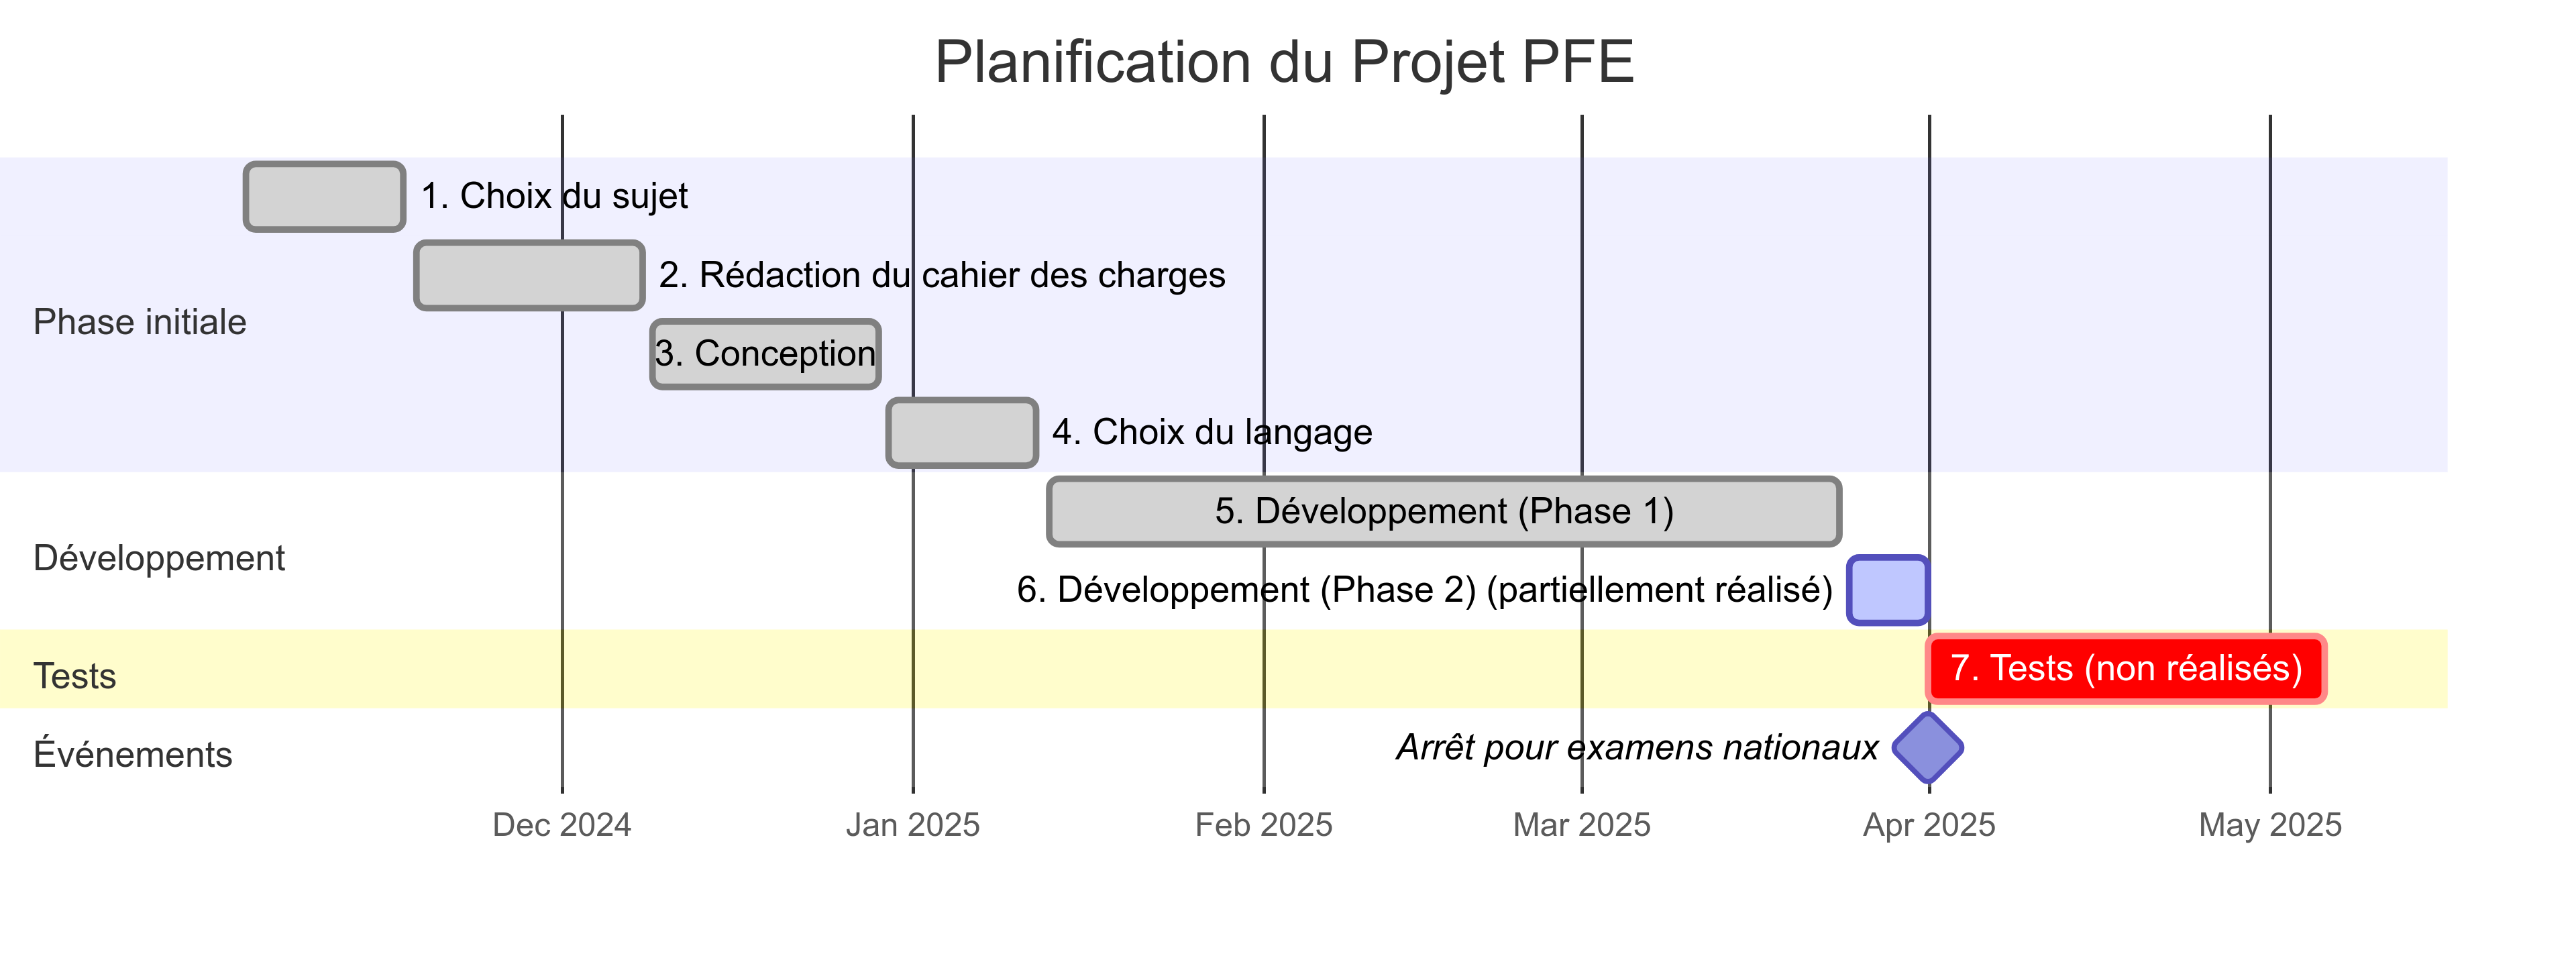
\includegraphics[width=1.0\textwidth,keepaspectratio]{pfe-pics/diagrames/Mermaid Chart - Create complex, visual diagrams with text. A smarter way of creating diagrams.-2025-06-10-203842.png}
  \caption{\textbf{Diagramme de Gantt} montrant la planification temporelle du projet.}
  \label{fig:gantt_chart}
\end{figure}

\subsection{Dépendances et chemin critique}

Le diagramme PERT ci-dessous illustre les dépendances entre les différentes tâches du projet et met en évidence le chemin critique:

\begin{figure}[H]
  \centering
  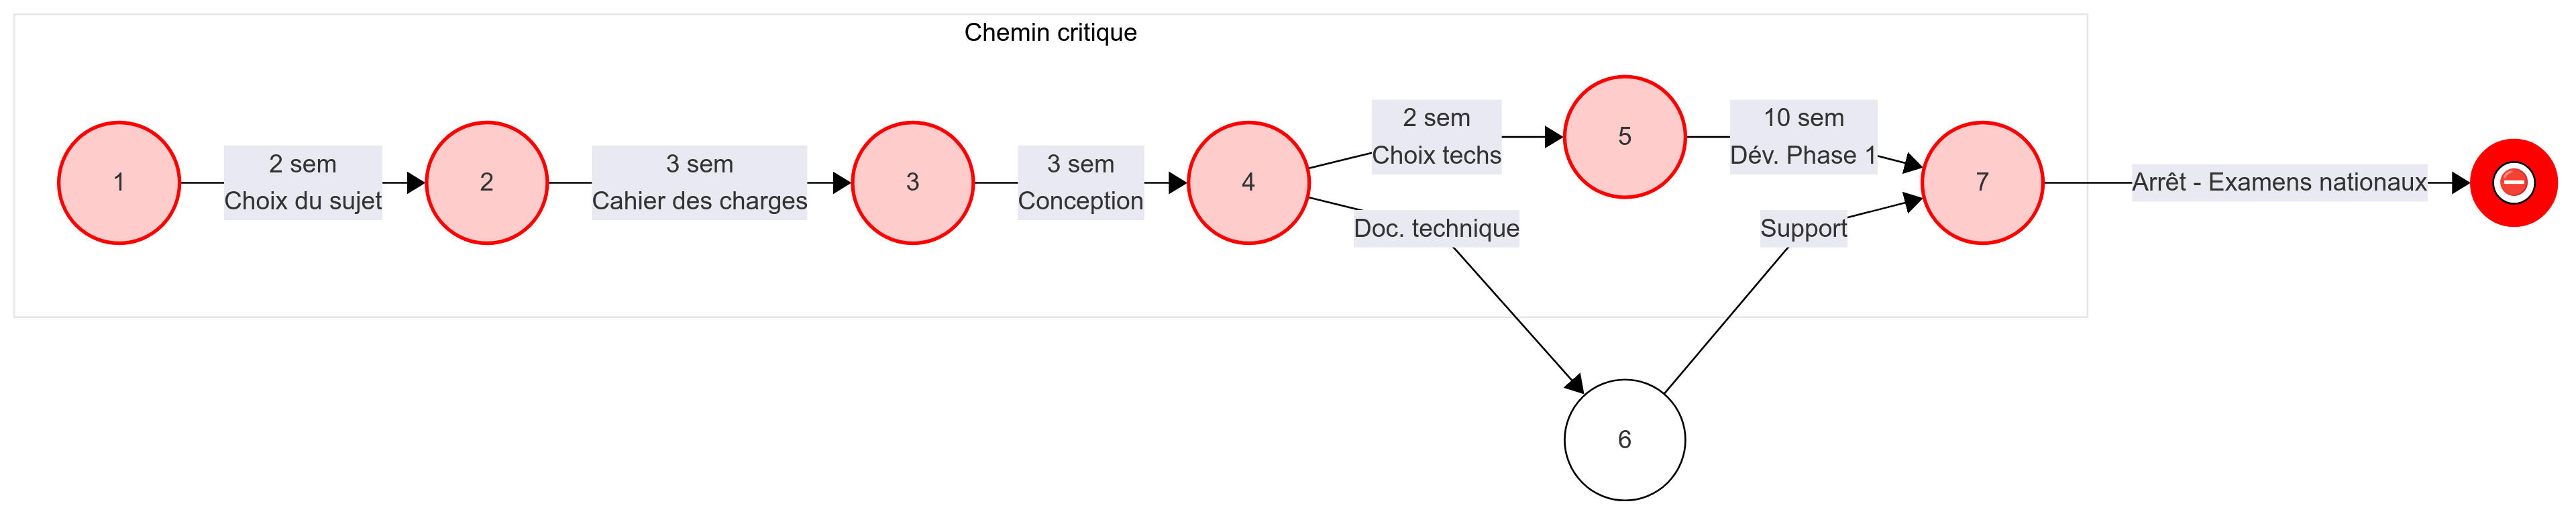
\includegraphics[width=1.0\textwidth,keepaspectratio]{pfe-pics/diagrames/Mermaid Chart - Create complex, visual diagrams with text. A smarter way of creating diagrams.-2025-06-10-203658.png}
  \caption{\textbf{Diagramme PERT} illustrant les dépendances et le chemin critique du projet.}
  \label{fig:pert_diagram}
\end{figure}

Ce diagramme met en évidence:

\begin{itemize}
  \item Les relations de précédence entre les activités
  
  \item Le chemin critique déterminant la durée minimale du projet
  
  \item Les marges disponibles pour certaines activités non critiques
  
  \item Les points de synchronisation nécessaires entre les différents volets du projet
\end{itemize}

\subsection{Répartition des tâches}

L'équipe de projet a été organisée selon les compétences de chaque membre:

\begin{itemize}
  \item \textbf{Architecture et conception}: Définition de l'architecture globale et des modèles de données
  
  \item \textbf{Développement backend}: Implémentation des API et services métier
  
  \item \textbf{Développement frontend web}: Création des interfaces utilisateur web
  
  \item \textbf{Développement mobile}: Réalisation des applications mobiles
  
  \item \textbf{Intelligence artificielle}: Conception et implémentation du système de profils IA
  
  \item \textbf{Tests et qualité}: Validation des fonctionnalités et correction des anomalies
  
  \item \textbf{Documentation}: Rédaction des guides et de la documentation technique
\end{itemize}

\section{Conclusion du cahier des charges}

Ce cahier des charges définit les contours de notre projet de fin d'études, qui vise à développer deux systèmes complémentaires pour moderniser l'environnement éducatif:

\begin{itemize}
  \item Un système de gestion scolaire complet couvrant les besoins administratifs et pédagogiques des établissements
  
  \item Une plateforme innovante de création de profils IA pour enrichir l'expérience d'apprentissage
\end{itemize}

L'approche choisie, combinant des technologies modernes et une méthodologie agile, permettra de livrer des solutions robustes, évolutives et adaptées aux besoins des différents utilisateurs. L'intégration des deux systèmes offrira une valeur ajoutée unique, positionnant ce projet à l'intersection de la gestion éducative traditionnelle et de l'innovation par l'intelligence artificielle.

Les spécifications détaillées dans ce document serviront de référence tout au long du développement, tout en permettant les ajustements nécessaires pour s'adapter aux retours des utilisateurs et aux contraintes techniques qui pourraient émerger. 
\chapter*{Chapitre 2 : Architecture et conception du système}
\addcontentsline{toc}{chapter}{Chapitre 2 : Architecture et conception du système}
\thispagestyle{fancy}
\setcounter{section}{0}
\newpage

\section{Approche architecturale globale}

La conception de nos deux systèmes complémentaires a été guidée par des principes modernes d'architecture logicielle, visant à créer des solutions robustes, évolutives et maintenables.

\subsection{Vision architecturale}

Notre approche architecturale repose sur plusieurs principes fondamentaux :

\begin{itemize}
  \item \textbf{Séparation des préoccupations} : Distinction claire entre les différentes couches et composants du système
  
  \item \textbf{Modularité} : Organisation en modules indépendants et faiblement couplés
  
  \item \textbf{Scalabilité horizontale} : Capacité à augmenter les performances en ajoutant des instances de service
  
  \item \textbf{Résilience} : Tolérance aux pannes et récupération automatique
  
  \item \textbf{Sécurité par conception} : Intégration des considérations de sécurité à chaque niveau
\end{itemize}

\subsection{Architecture du système de gestion scolaire}

Le système de gestion scolaire adopte une architecture multicouche moderne avec une séparation claire entre frontend et backend :

\begin{figure}[H]
  \centering
  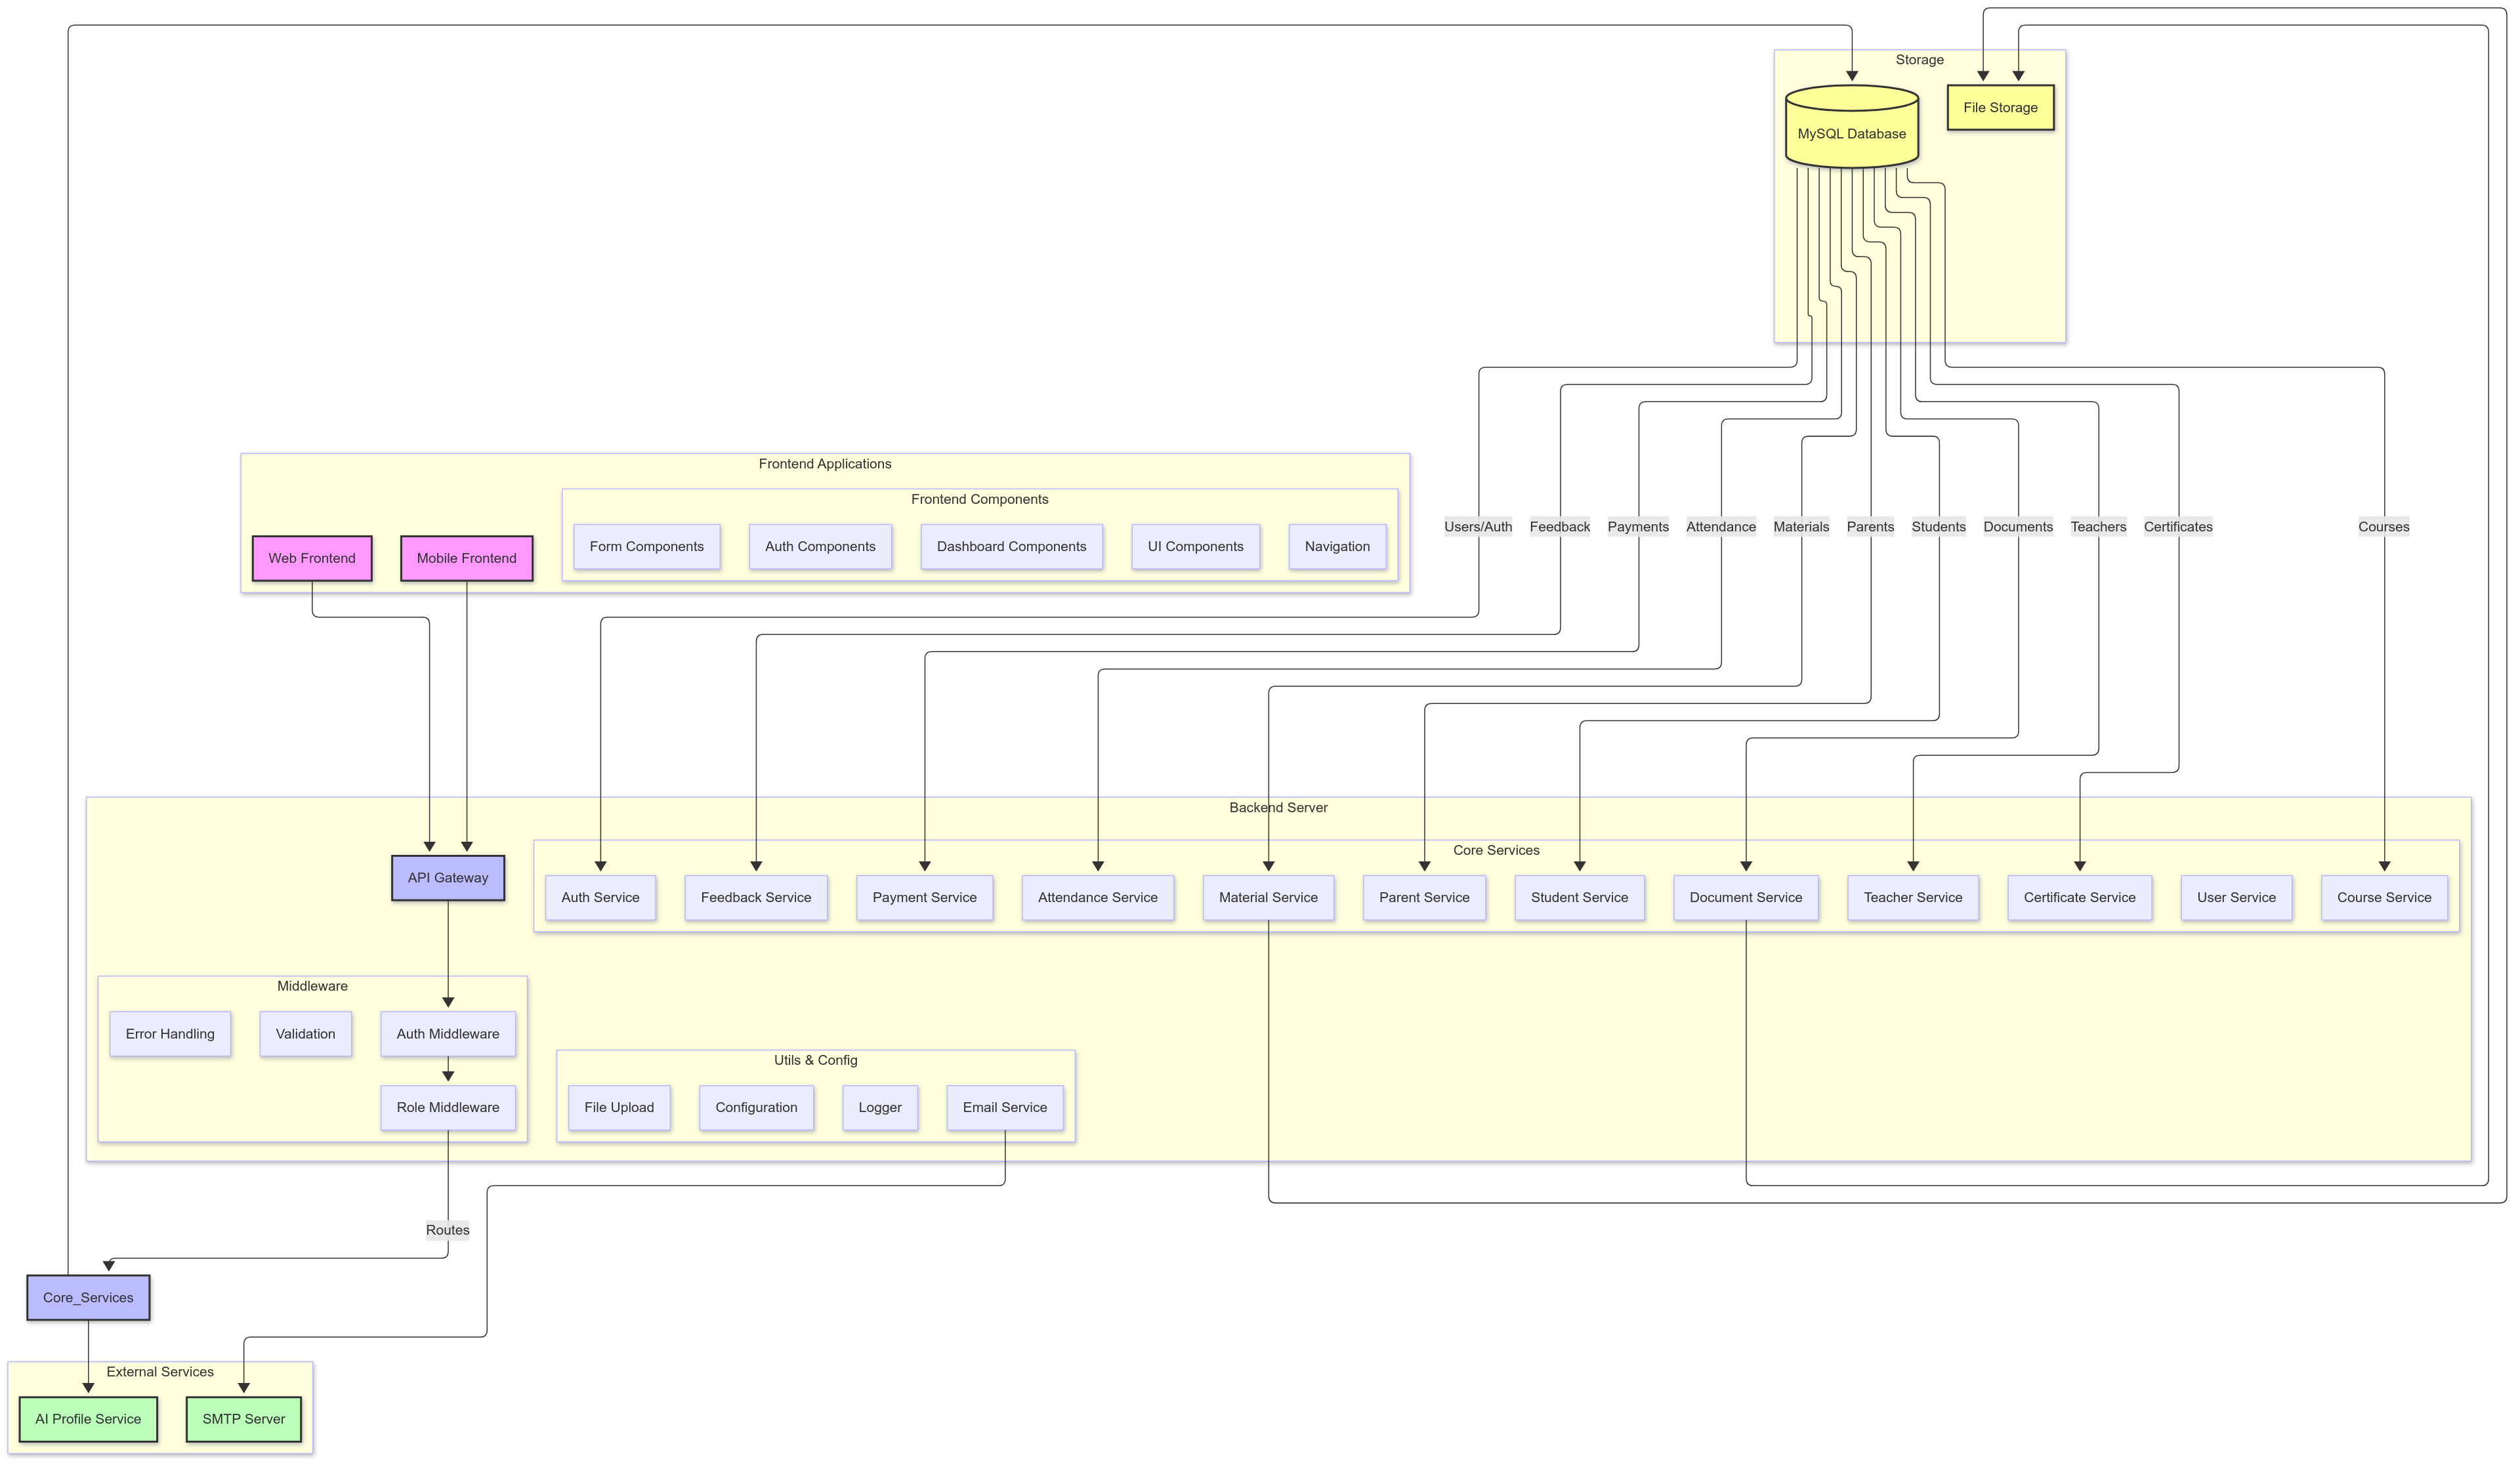
\includegraphics[width=0.9\textwidth,keepaspectratio]{pfe-pics/diagrames/archetecture.png}
  \caption{\textbf{Architecture globale} du système de gestion scolaire.}
  \label{fig:school_architecture}
\end{figure}

Cette architecture se compose de :

\begin{itemize}
  \item \textbf{Couche présentation} : Applications web et mobile offrant des interfaces adaptées à chaque type d'utilisateur
  
  \item \textbf{Couche API} : Services RESTful sécurisés exposant les fonctionnalités du système
  
  \item \textbf{Couche métier} : Implémentation de la logique métier et des règles de gestion
  
  \item \textbf{Couche persistance} : Gestion des données et interactions avec la base de données
  
  \item \textbf{Services transversaux} : Authentification, journalisation, gestion des fichiers, etc.
\end{itemize}

\subsection{Architecture du système de création de profils IA}

Le système de création de profils IA s'appuie sur une architecture orientée services, optimisée pour le traitement de documents et l'interaction avec des modèles d'IA :

\begin{itemize}
  \item \textbf{Frontend React/TypeScript} : Interface utilisateur réactive pour la gestion des profils et l'interaction avec l'IA
  
  \item \textbf{Backend FastAPI} : Services Python haute performance pour le traitement des documents et l'orchestration des modèles d'IA
  
  \item \textbf{Pipeline de traitement} : Système de traitement asynchrone pour l'extraction et l'analyse des contenus documentaires
  
  \item \textbf{Stockage hybride} : Combinaison de base de données PostgreSQL pour les métadonnées et de stockage objet pour les documents
  
  \item \textbf{Intégration IA} : Connecteurs vers des services d'IA externes (OpenRouter) pour le traitement du langage naturel
\end{itemize}

\section{Conception détaillée du système de gestion scolaire}

\subsection{Modèle de données}

Le modèle de données du système de gestion scolaire a été conçu pour représenter efficacement toutes les entités du domaine éducatif et leurs relations :

\begin{figure}[H]
  \centering
  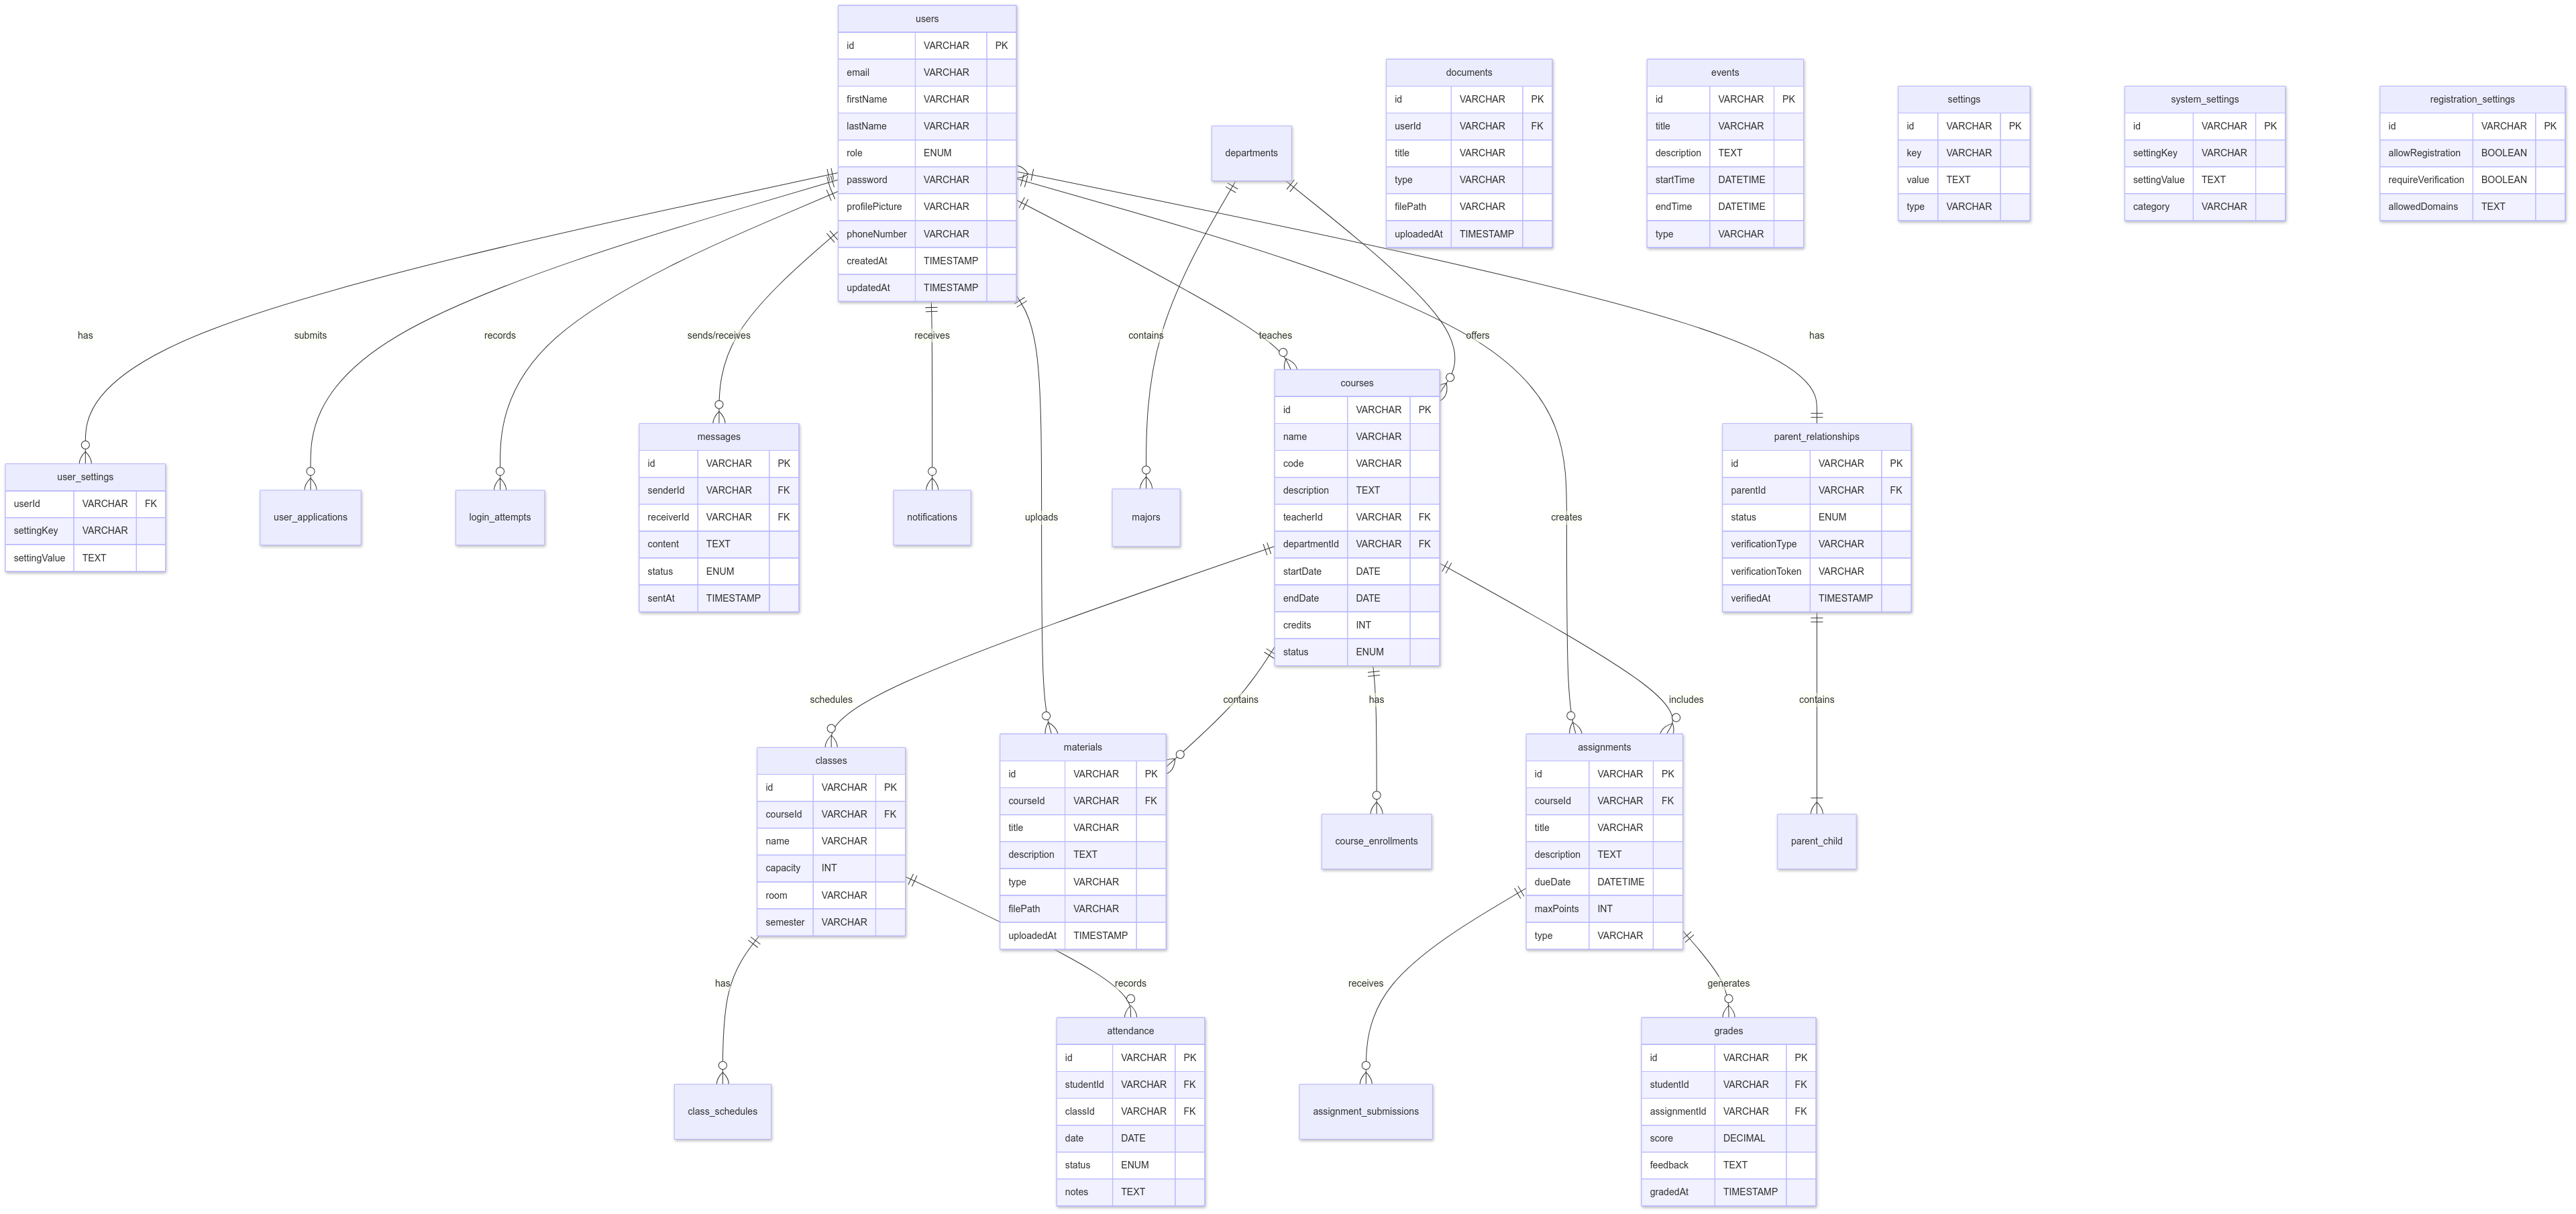
\includegraphics[width=0.9\textwidth,keepaspectratio]{pfe-pics/diagrames/tabaales.png}
  \caption{\textbf{Modèle de données} du système de gestion scolaire.}
  \label{fig:school_data_model}
\end{figure}

Les principales entités du modèle sont :

\begin{itemize}
  \item \textbf{User} : Entité de base pour tous les utilisateurs du système, avec spécialisation par rôle
  
  \item \textbf{Student} : Informations spécifiques aux étudiants, incluant leur parcours académique
  
  \item \textbf{Teacher} : Données relatives aux enseignants, incluant leurs spécialités et disponibilités
  
  \item \textbf{Parent} : Informations sur les parents et leurs relations avec les étudiants
  
  \item \textbf{Course} : Définition des cours avec leur contenu et organisation
  
  \item \textbf{Attendance} : Enregistrement des présences aux séances de cours
  
  \item \textbf{Assignment} : Travaux et évaluations assignés aux étudiants
  
  \item \textbf{Grade} : Notes et évaluations des étudiants
  
  \item \textbf{Notification} : Messages et alertes envoyés aux utilisateurs
  
  \item \textbf{Document} : Ressources pédagogiques et administratives partagées
\end{itemize}

\subsection{Diagramme de classes}

Le diagramme de classes détaille la structure objet du système et les relations entre les différentes classes :

\begin{figure}[H]
  \centering
  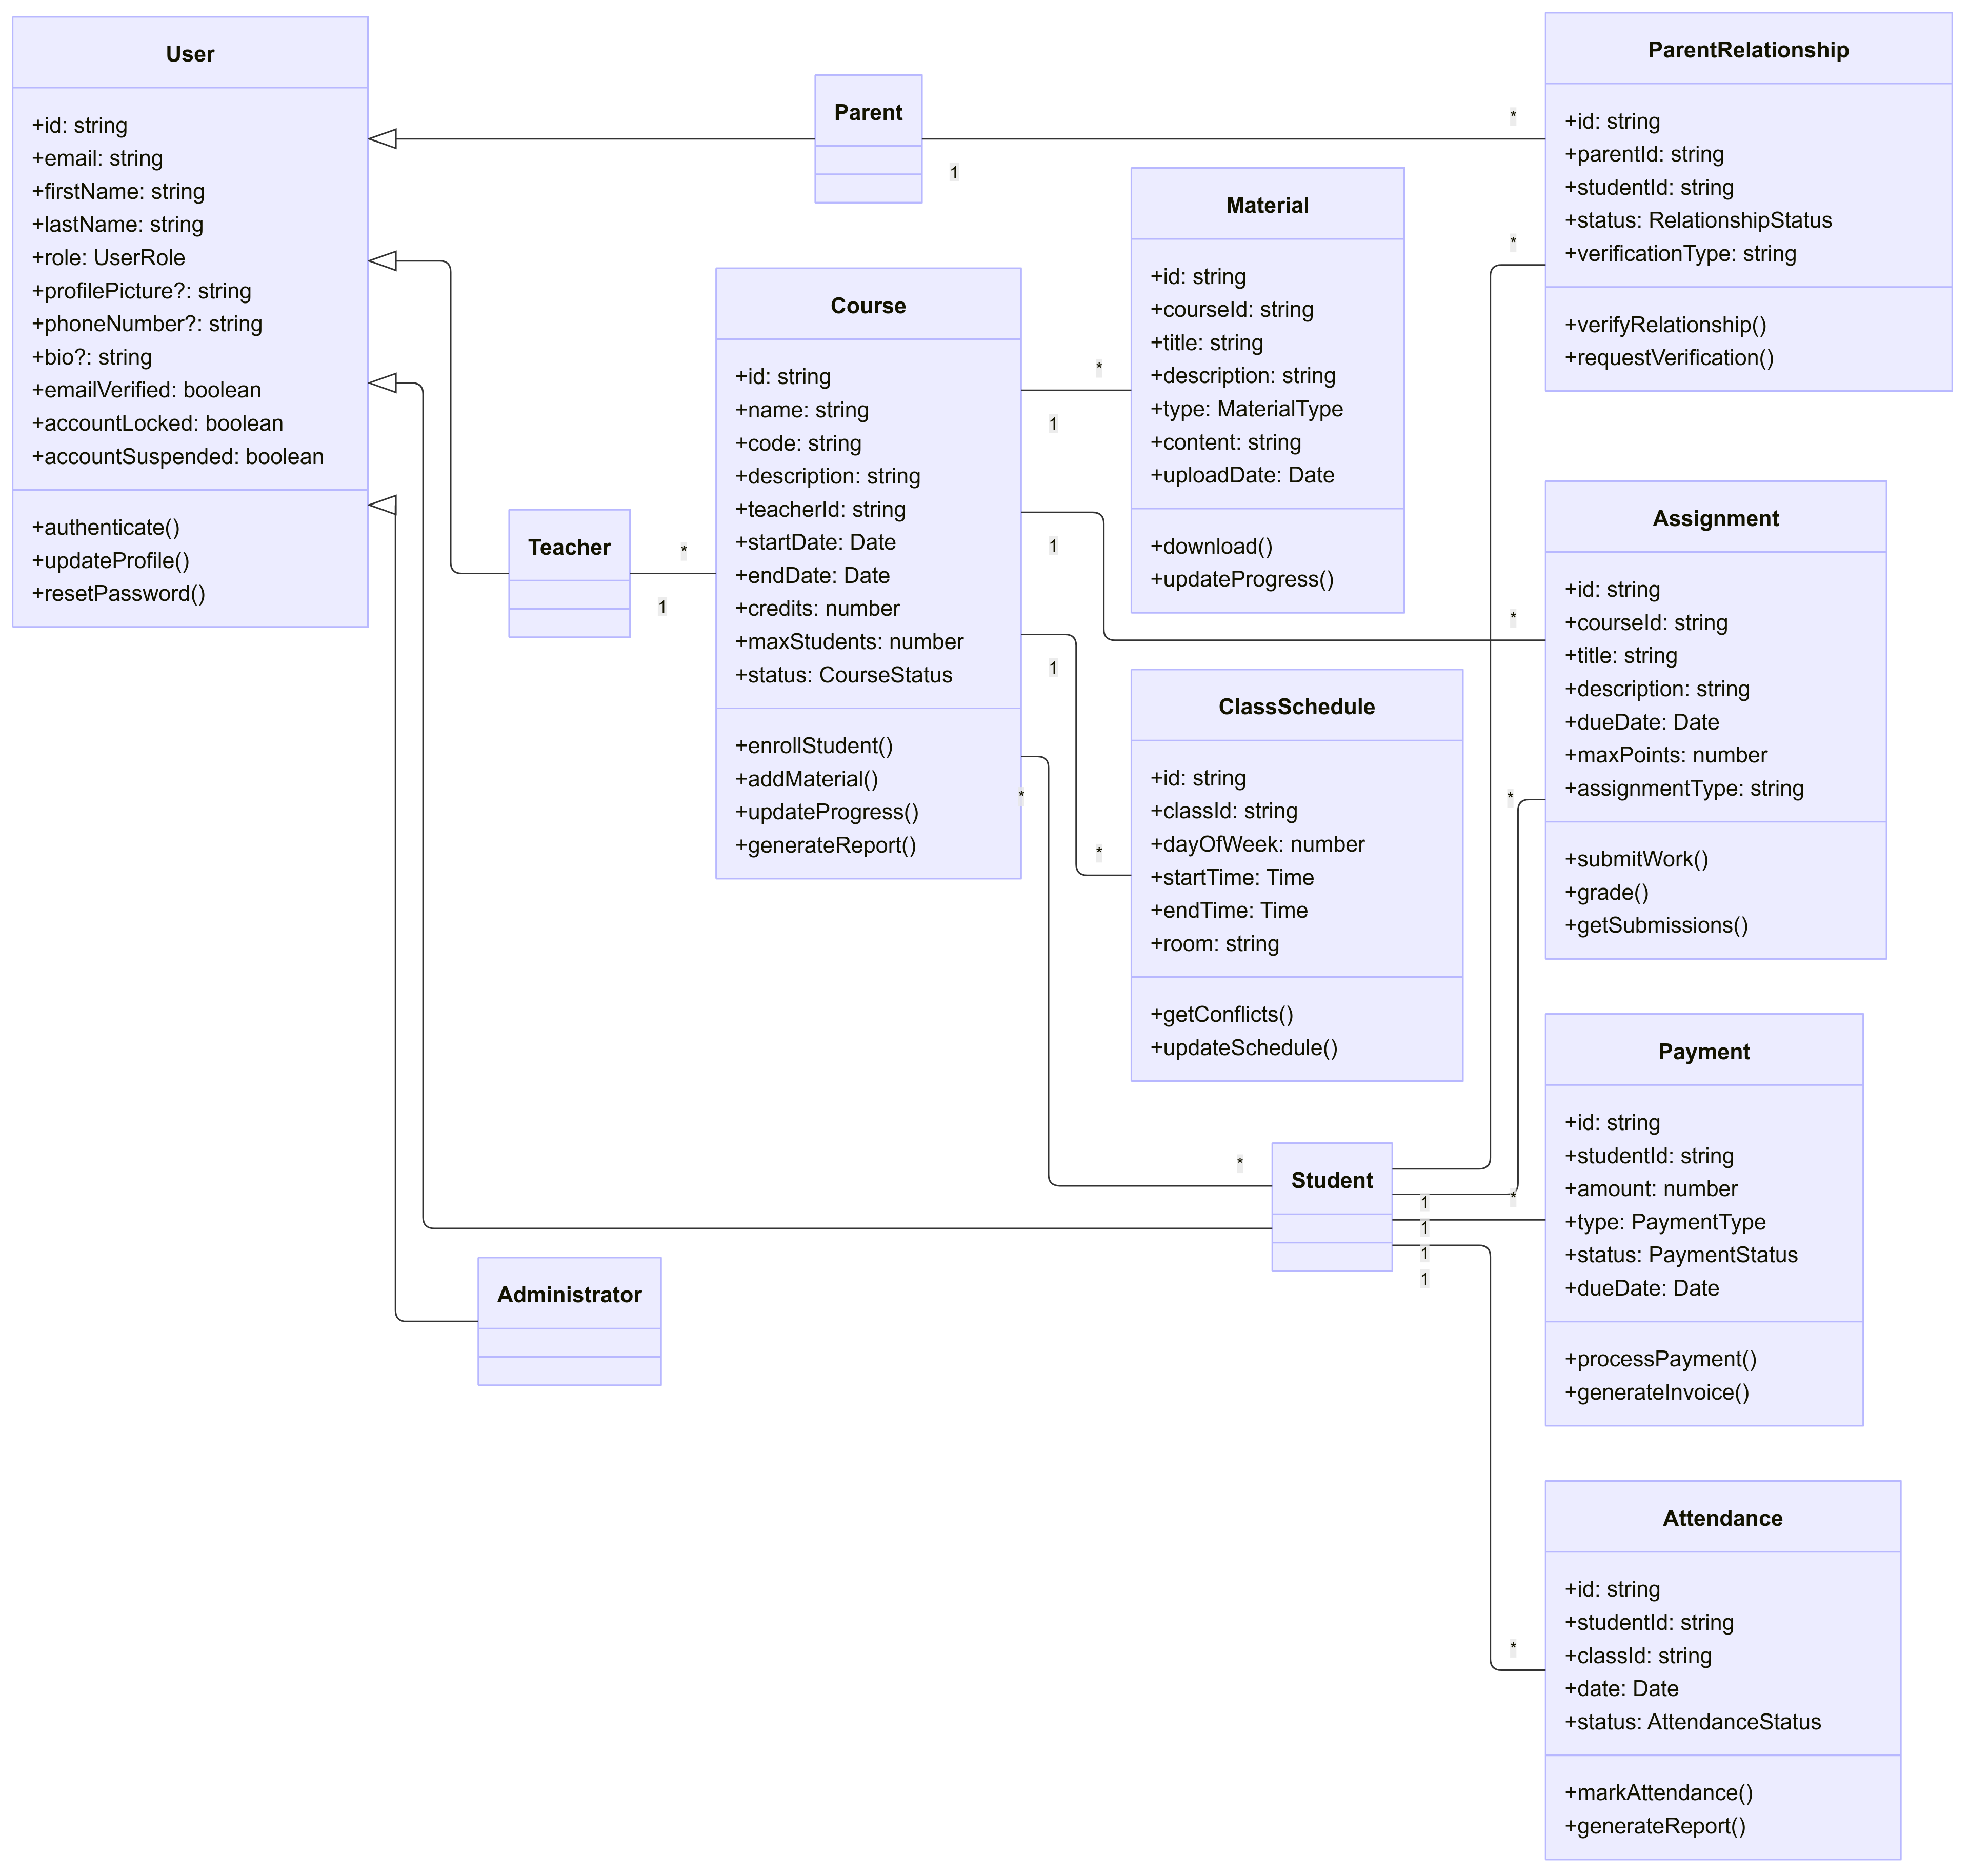
\includegraphics[width=0.9\textwidth,keepaspectratio]{pfe-pics/diagrames/class.png}
  \caption{\textbf{Diagramme de classes} du système de gestion scolaire.}
  \label{fig:school_class_diagram}
\end{figure}

Ce diagramme met en évidence :

\begin{itemize}
  \item Les attributs et méthodes clés de chaque classe
  
  \item Les relations d'héritage, notamment pour les différents types d'utilisateurs
  
  \item Les associations entre classes, avec leur cardinalité
  
  \item Les agrégations et compositions représentant les relations de contenance
\end{itemize}

\subsection{Architecture frontend}

L'architecture frontend du système de gestion scolaire repose sur une approche modulaire et réactive :

\subsubsection{Application web}

L'application web utilise React avec TypeScript et adopte une architecture basée sur les composants :

\begin{itemize}
  \item \textbf{Structure des composants} : Organisation hiérarchique avec composants atomiques, moléculaires et organismes
  
  \item \textbf{Gestion d'état} : Utilisation de Context API et hooks personnalisés pour la gestion de l'état global
  
  \item \textbf{Routage} : Système de navigation basé sur React Router avec gestion des autorisations
  
  \item \textbf{Thème et styles} : Approche basée sur Tailwind CSS avec thèmes personnalisables
  
  \item \textbf{Internationalisation} : Support multilingue avec gestion des traductions
\end{itemize}

\subsubsection{Application mobile}

L'application mobile est développée avec React Native, partageant une partie de la logique avec l'application web :

\begin{itemize}
  \item \textbf{Navigation native} : Utilisation de React Navigation pour une expérience fluide
  
  \item \textbf{Composants adaptatifs} : Interface optimisée pour les interactions tactiles
  
  \item \textbf{Fonctionnalités natives} : Intégration des notifications push, de l'appareil photo et du stockage local
  
  \item \textbf{Mode hors ligne} : Synchronisation des données pour utilisation sans connexion permanente
\end{itemize}

\subsection{Architecture backend}

Le backend du système de gestion scolaire est conçu selon une architecture en couches avec une séparation claire des responsabilités :

\begin{itemize}
  \item \textbf{Couche API} : Contrôleurs REST exposant les endpoints du système
  
  \item \textbf{Couche service} : Implémentation de la logique métier et orchestration des opérations
  
  \item \textbf{Couche repository} : Abstraction des opérations de persistance et requêtes à la base de données
  
  \item \textbf{Couche entité} : Modèles de données et mappings ORM
  
  \item \textbf{Services transversaux} : Authentification, autorisation, validation, journalisation
\end{itemize}

\subsection{Flux de travail principaux}

Plusieurs flux de travail clés ont été modélisés pour guider l'implémentation :

\subsubsection{Processus d'authentification}

\begin{figure}[H]
  \centering
  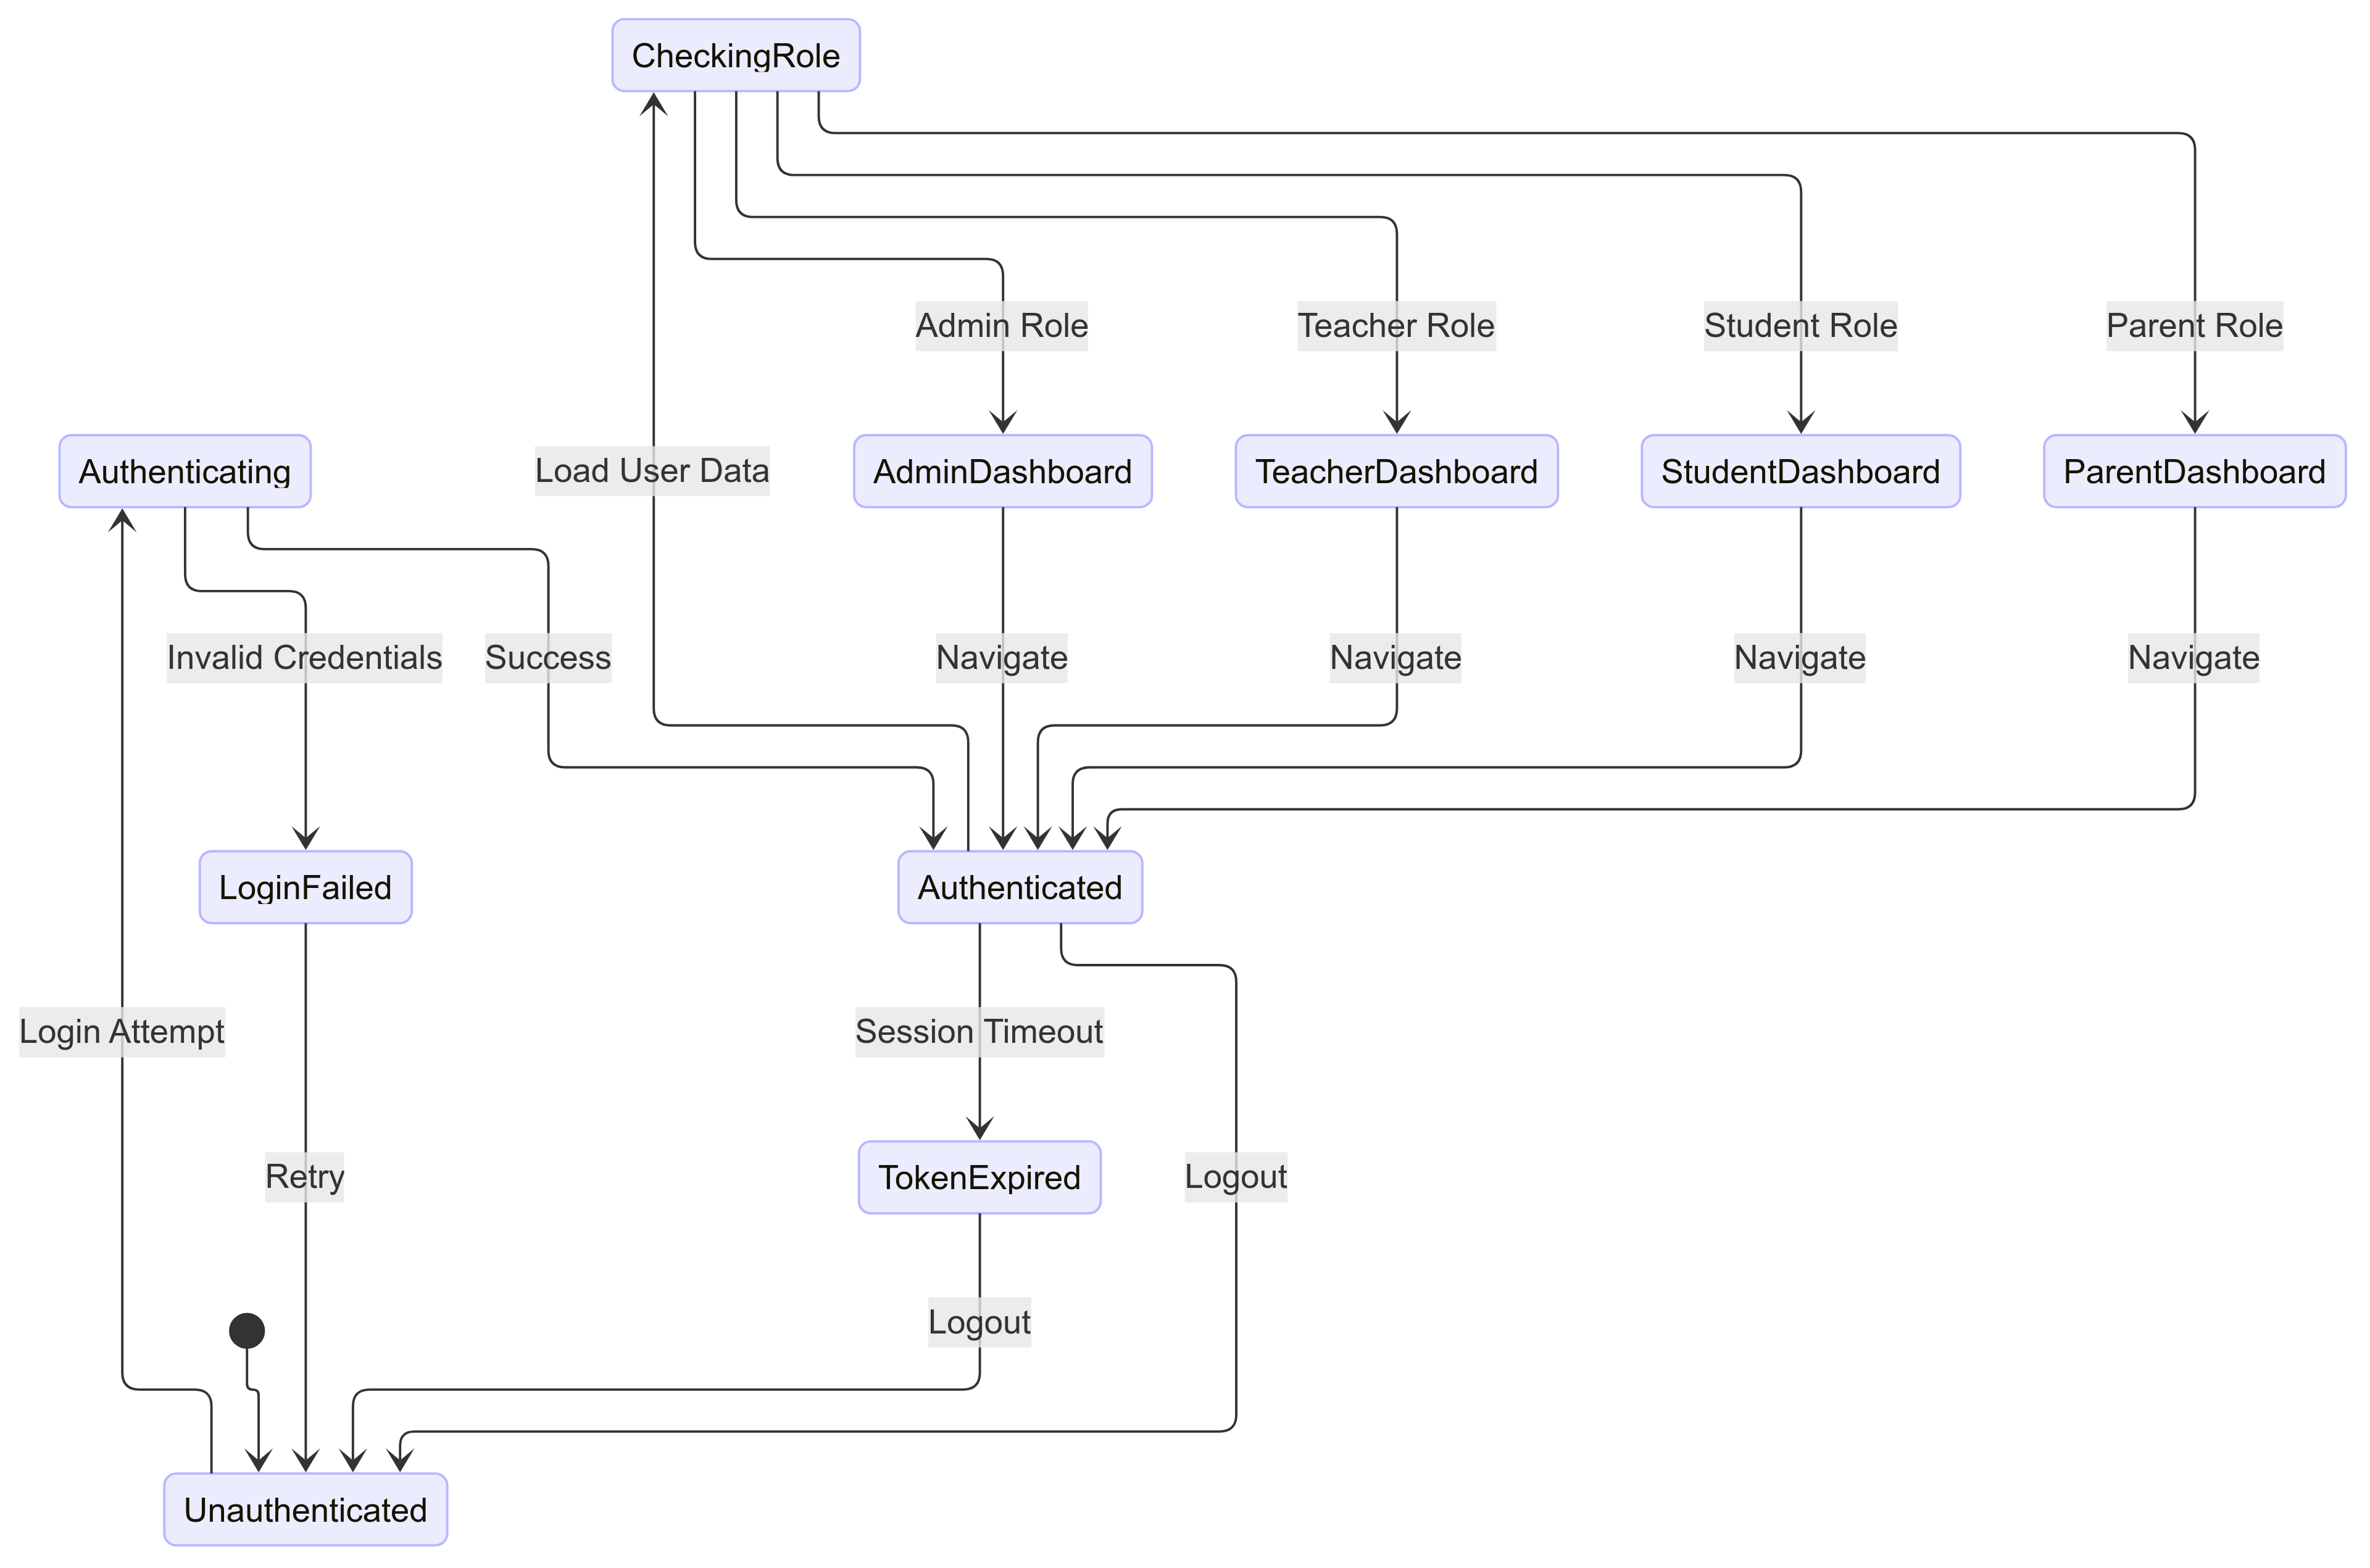
\includegraphics[width=0.9\textwidth,keepaspectratio]{pfe-pics/diagrames/State Diagram (for Authentication Flow).png}
  \caption{\textbf{Diagramme d'états} pour le processus d'authentification.}
  \label{fig:auth_flow}
\end{figure}

Ce diagramme illustre :

\begin{itemize}
  \item Les différents états possibles du processus d'authentification
  
  \item Les transitions entre ces états en fonction des actions utilisateur
  
  \item Les vérifications de sécurité à chaque étape
  
  \item La gestion des erreurs et des cas particuliers
\end{itemize}

\subsubsection{Gestion des cours}

\begin{figure}[H]
  \centering
  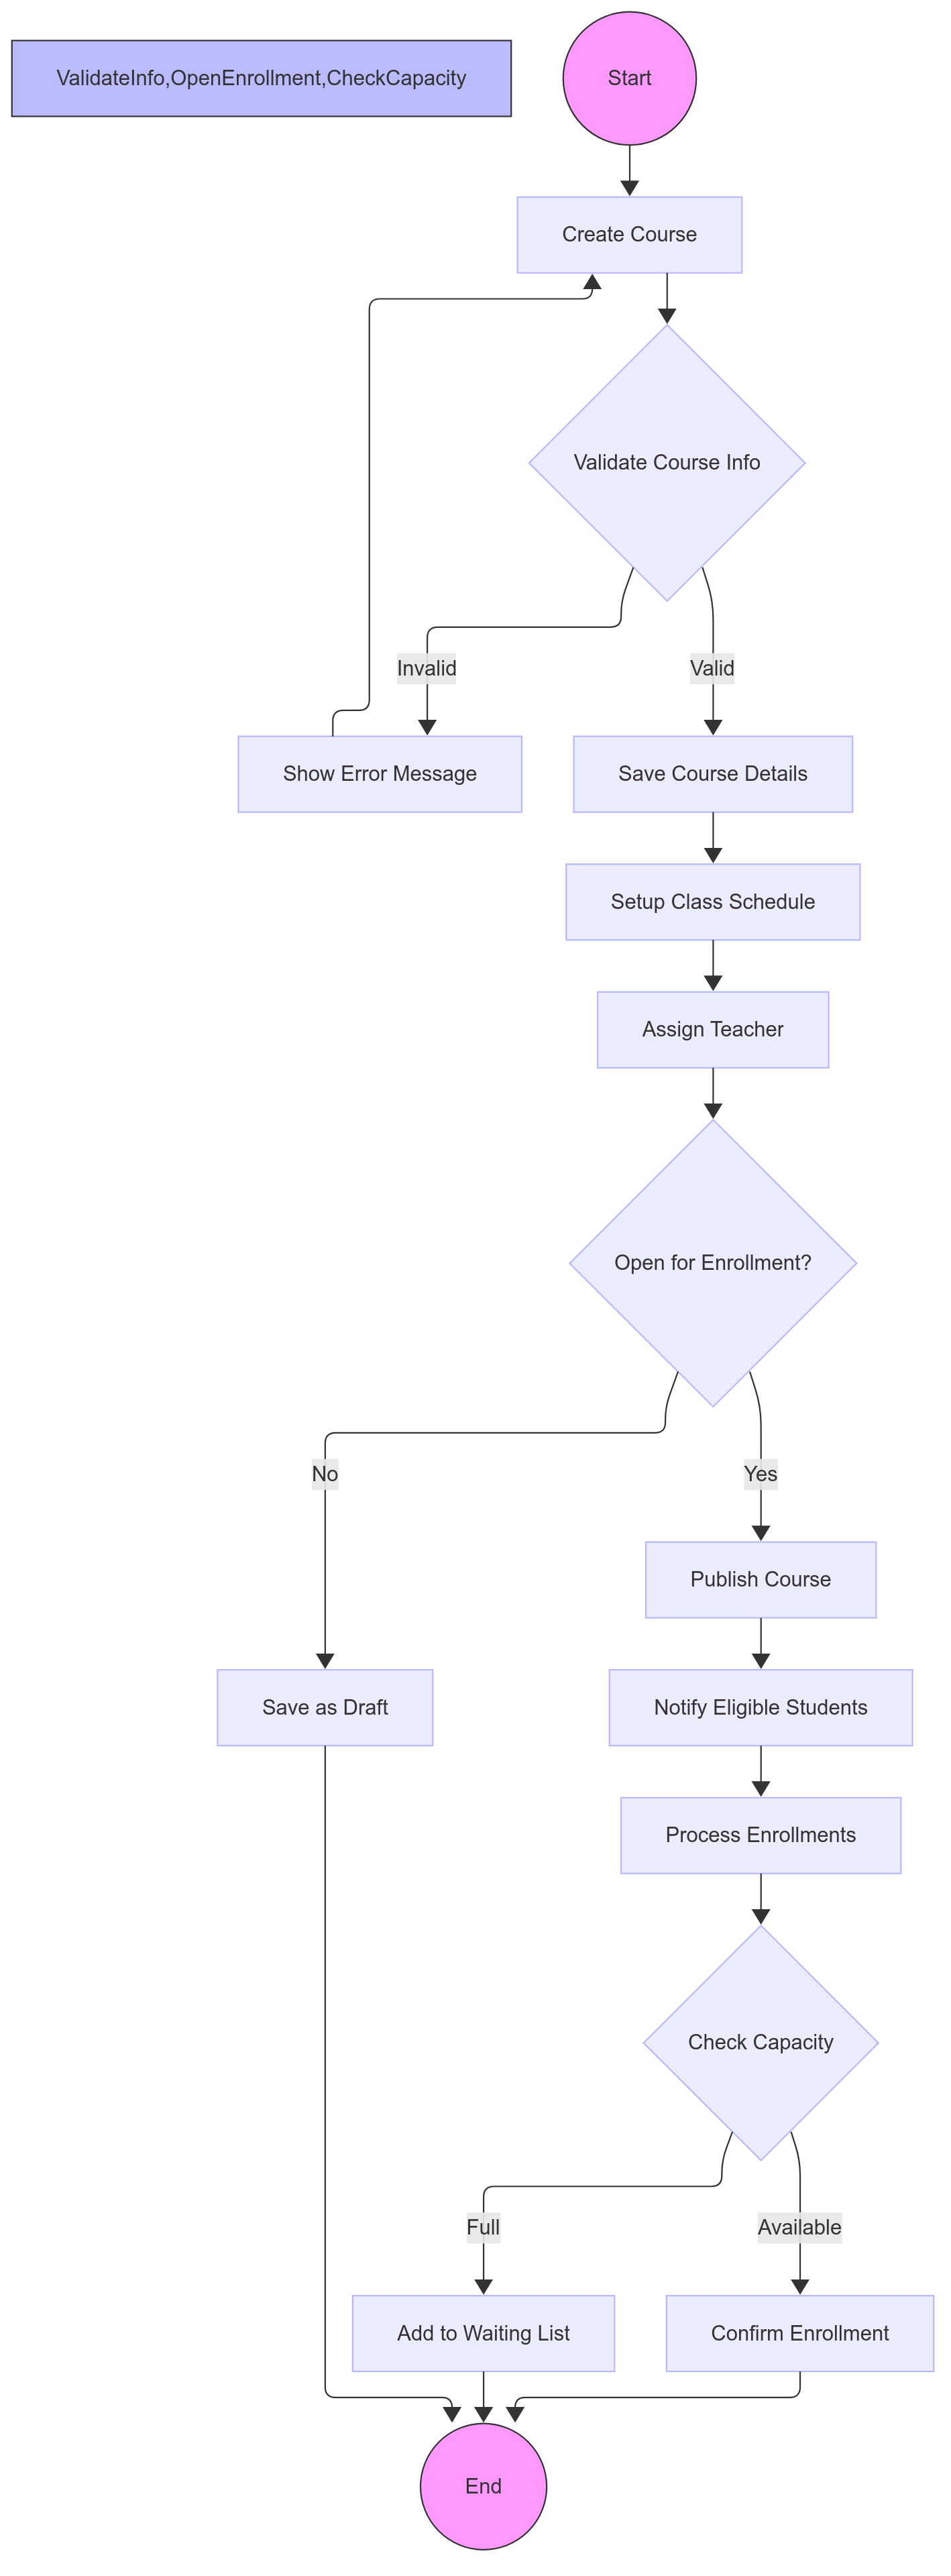
\includegraphics[width=0.7\textwidth,height=0.8\textheight,keepaspectratio]{pfe-pics/diagrames/Activity Diagram (for Course Management).png}
  \caption{\textbf{Diagramme d'activité} pour la gestion des cours.}
  \label{fig:course_management}
\end{figure}

Ce flux détaille :

\begin{itemize}
  \item Les étapes de création et configuration d'un cours
  
  \item L'assignation des enseignants et l'inscription des étudiants
  
  \item La gestion du matériel pédagogique
  
  \item Le suivi et l'évaluation des activités du cours
\end{itemize}

\subsubsection{Suivi des présences}

\begin{figure}[H]
  \centering
  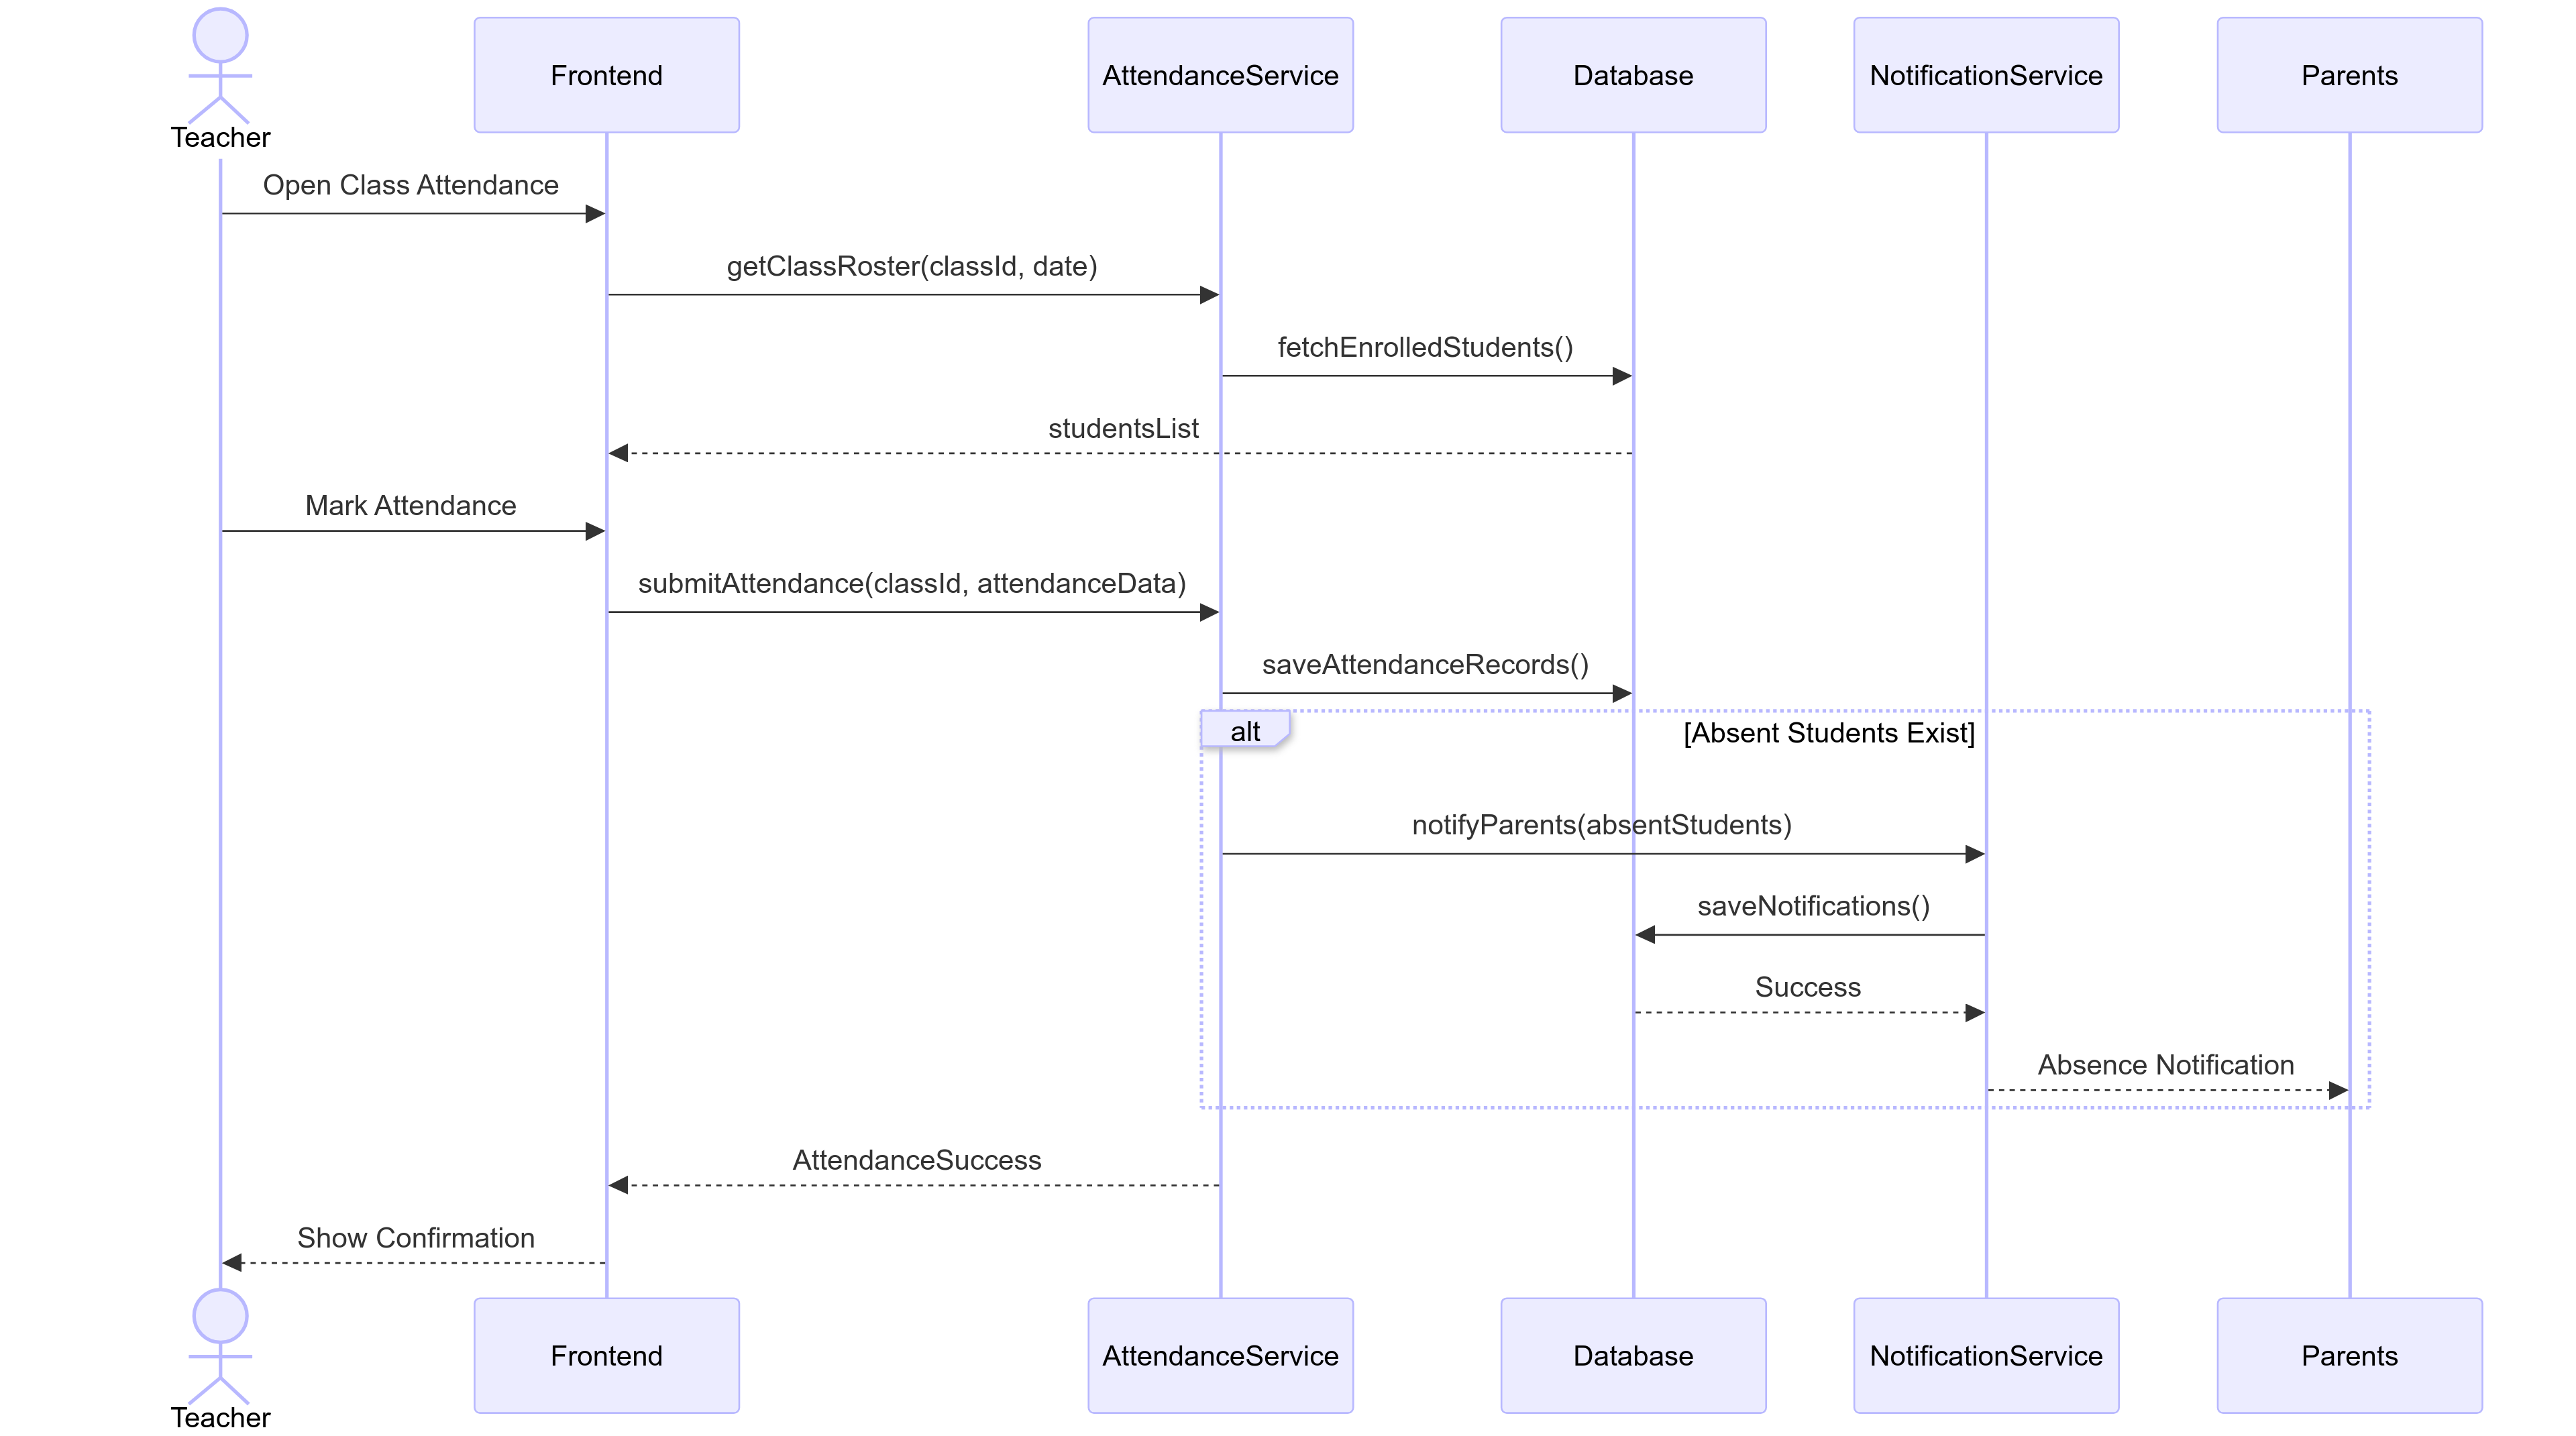
\includegraphics[width=0.9\textwidth,keepaspectratio]{pfe-pics/diagrames/Attendance Tracking.png}
  \caption{\textbf{Diagramme de séquence} pour le suivi des présences.}
  \label{fig:attendance_tracking}
\end{figure}

Ce diagramme montre :

\begin{itemize}
  \item Les interactions entre l'enseignant et le système pour l'enregistrement des présences
  
  \item La validation et la persistance des données d'assiduité
  
  \item Les notifications automatiques en cas d'absence
  
  \item La consultation des rapports de présence par les différents acteurs
\end{itemize}

\subsubsection{Soumission et notation des devoirs}

\begin{figure}[H]
  \centering
  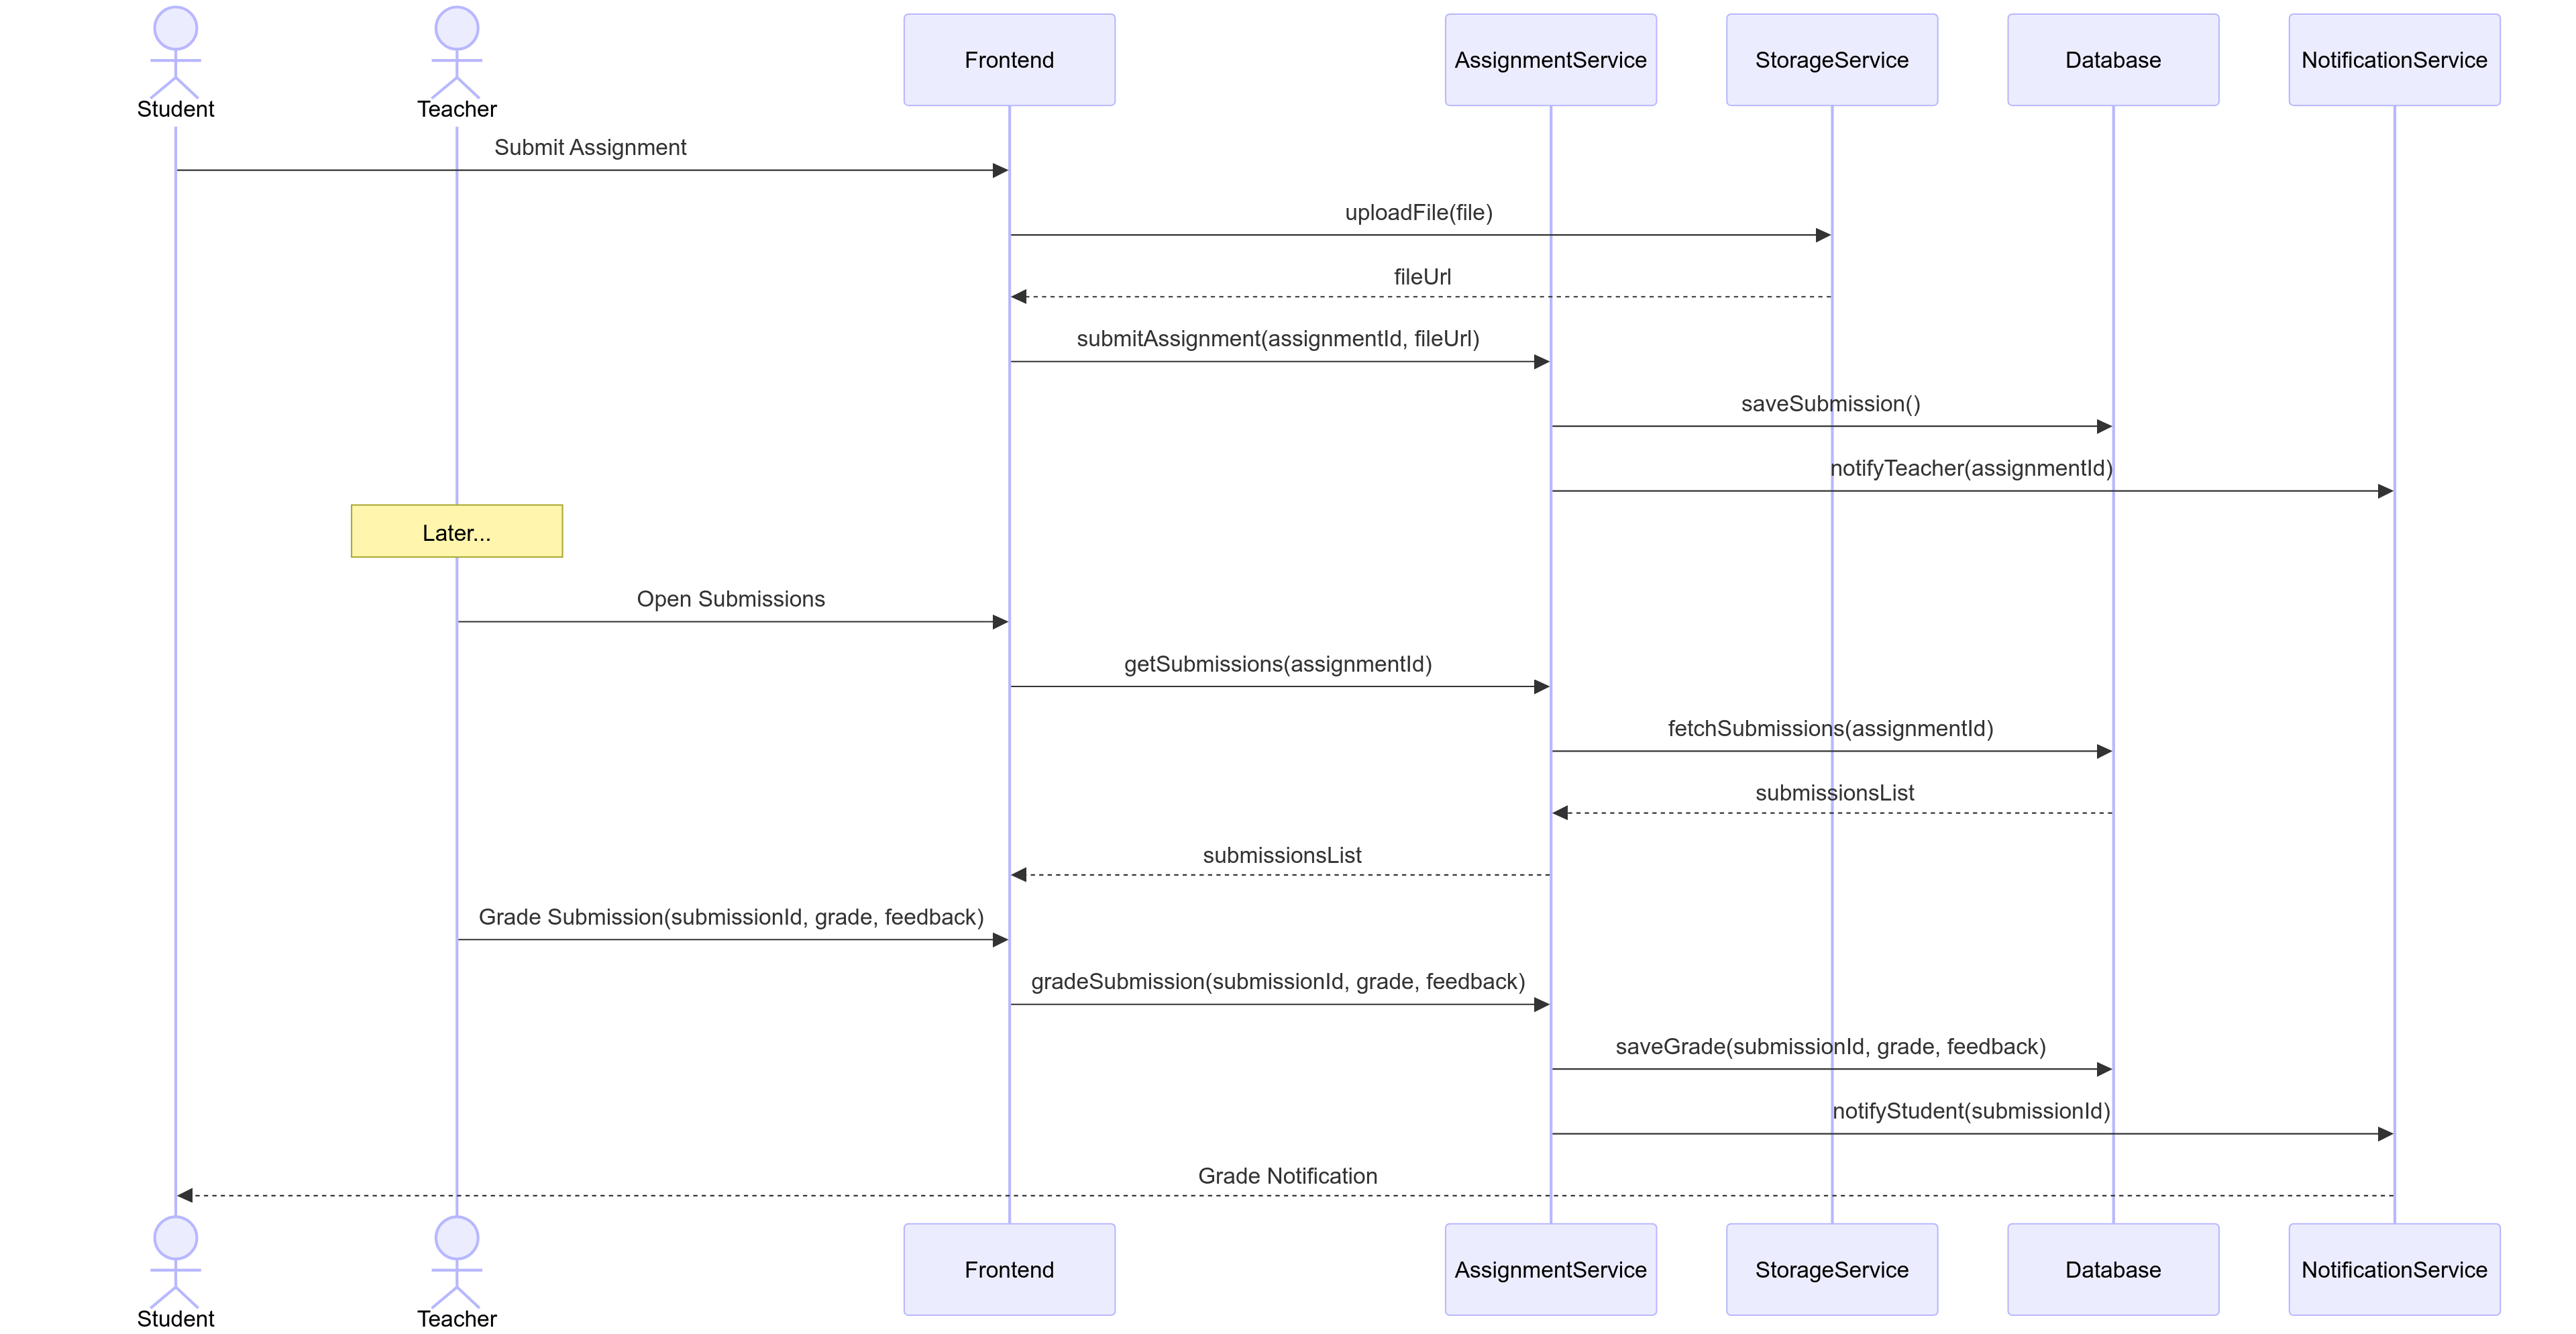
\includegraphics[width=0.9\textwidth,keepaspectratio]{pfe-pics/diagrames/Assignment Submission and Grading.png}
  \caption{\textbf{Diagramme de flux} pour la soumission et notation des devoirs.}
  \label{fig:assignment_grading}
\end{figure}

Ce flux illustre :

\begin{itemize}
  \item La création et l'assignation de travaux par l'enseignant
  
  \item La soumission des travaux par les étudiants
  
  \item Le processus d'évaluation et de feedback
  
  \item La publication et consultation des résultats
\end{itemize}

\subsubsection{Vérification parent-enfant}

\begin{figure}[H]
  \centering
  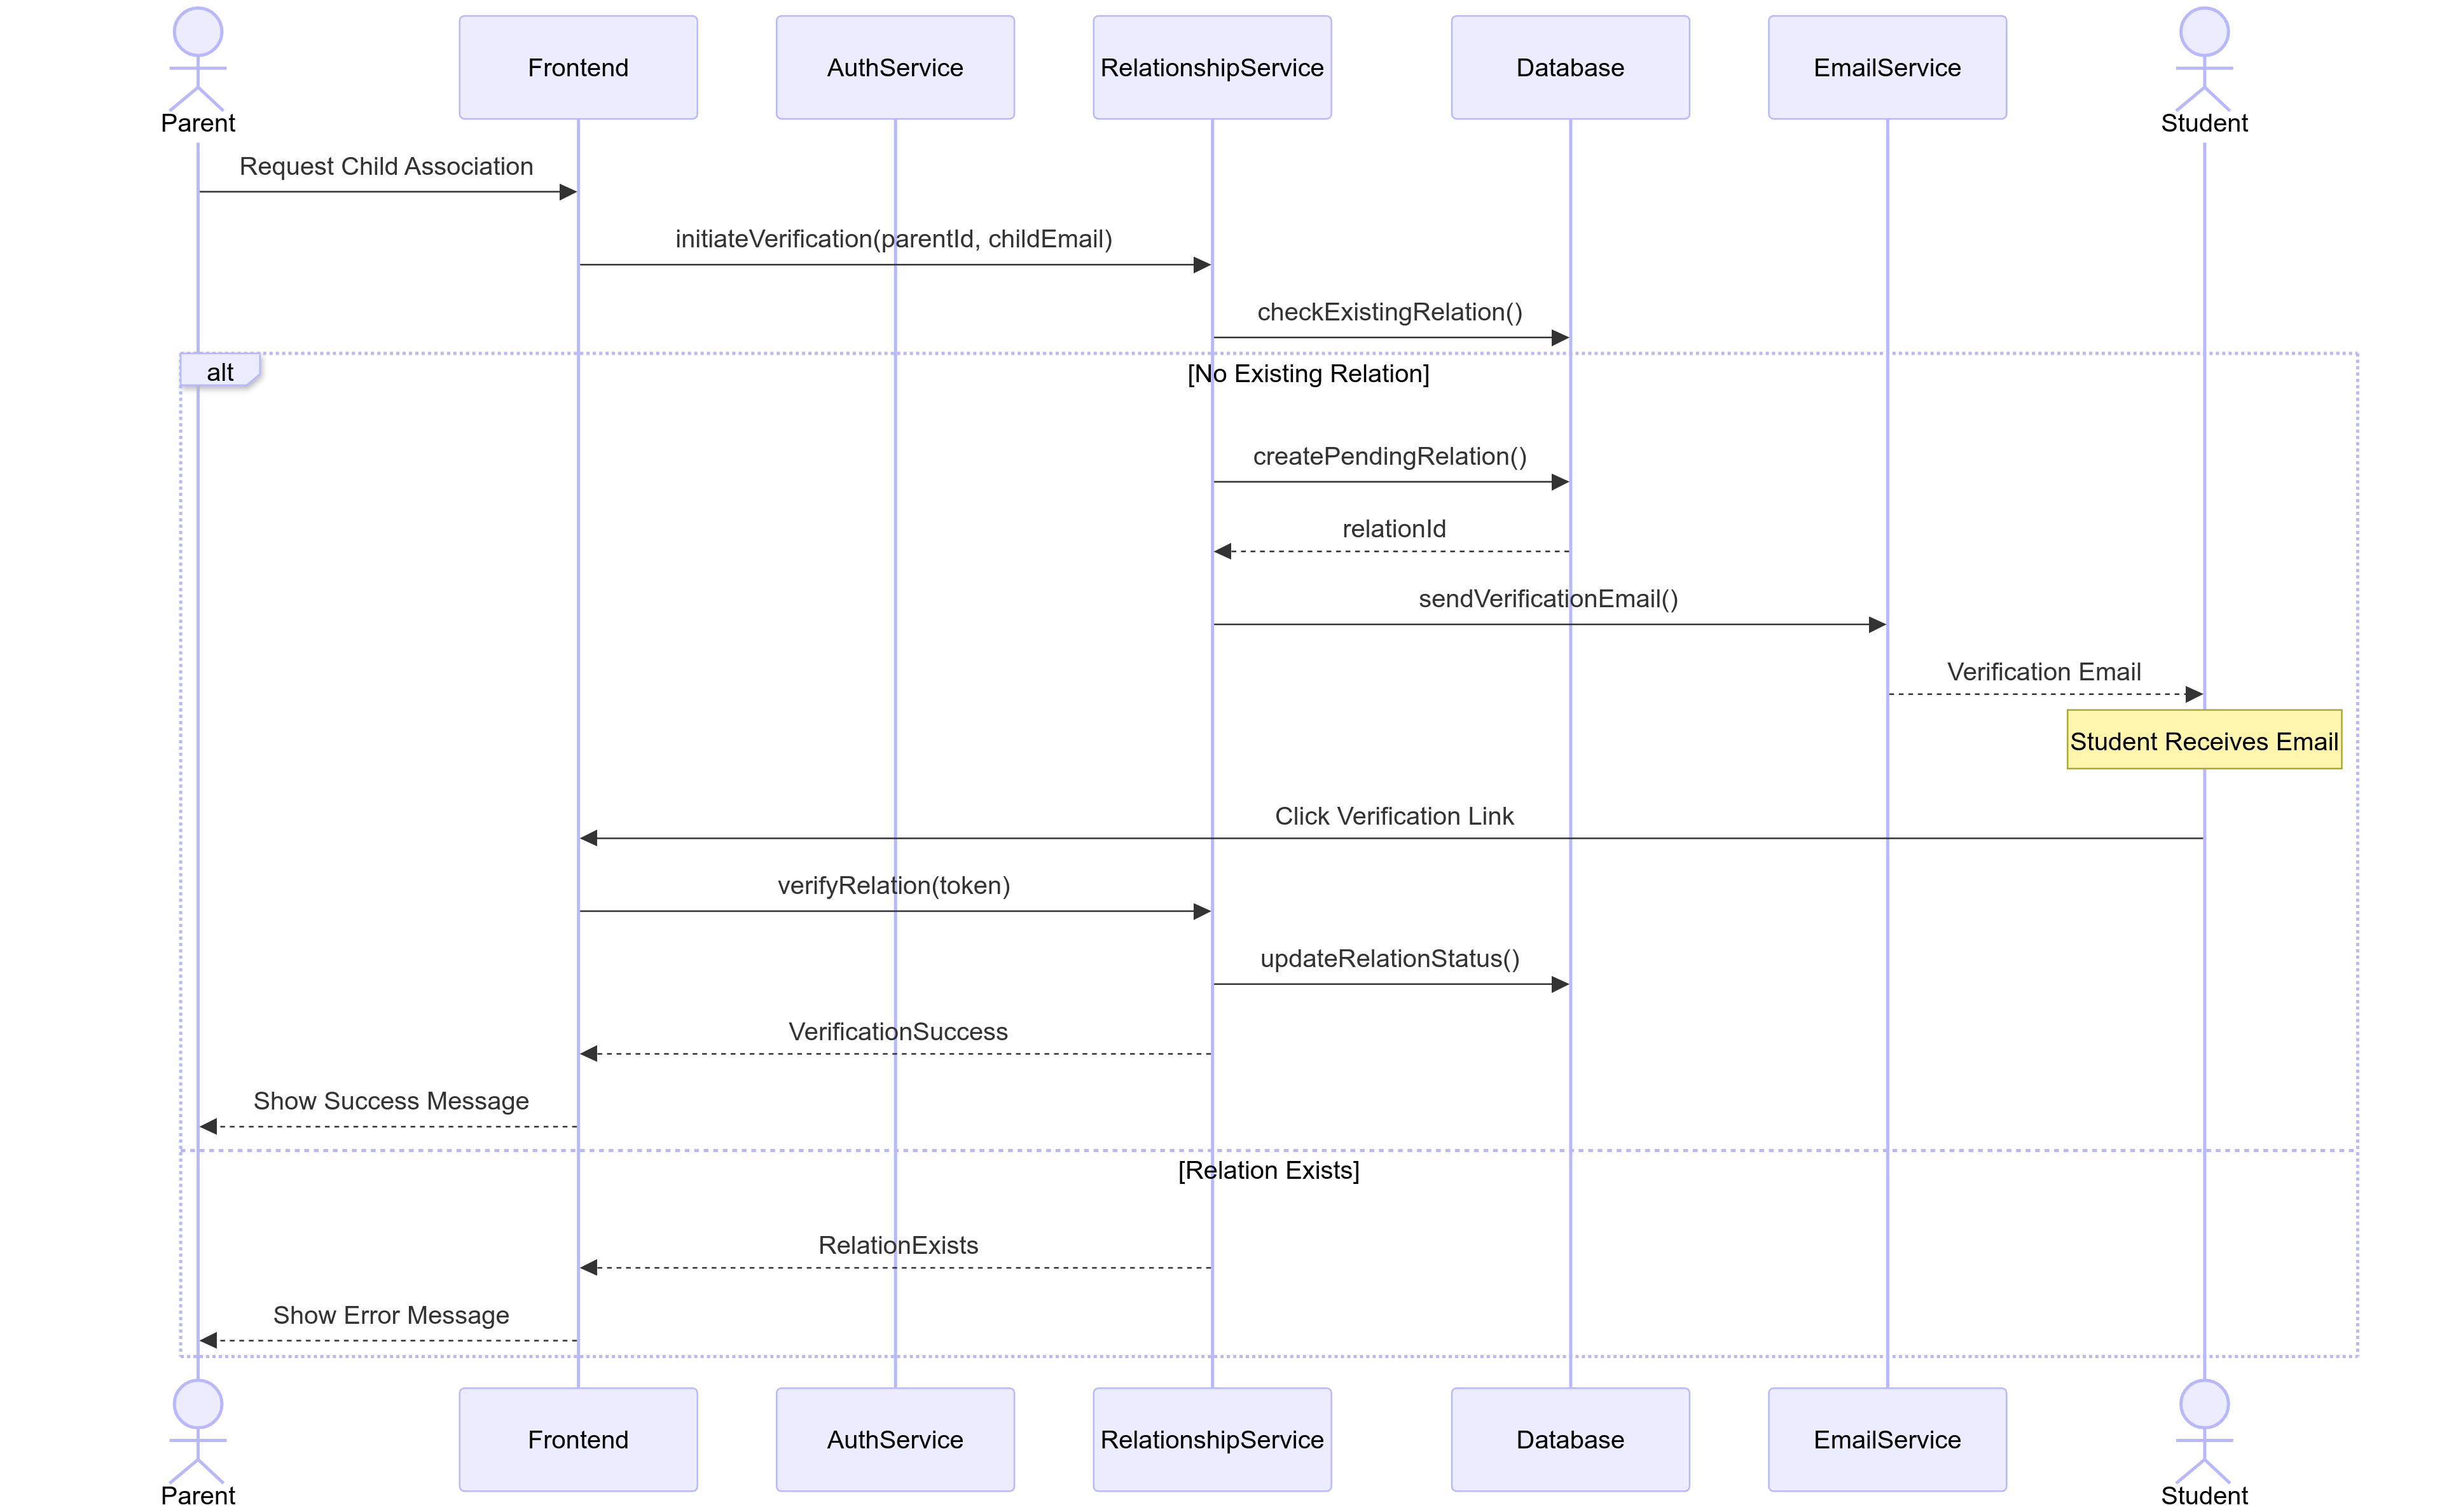
\includegraphics[width=0.9\textwidth,keepaspectratio]{pfe-pics/diagrames/Parent-Child Verification Process.png}
  \caption{\textbf{Diagramme de processus} pour la vérification parent-enfant.}
  \label{fig:parent_child_verification}
\end{figure}

Ce processus sécurisé détaille :

\begin{itemize}
  \item L'initiation de la demande d'association par le parent
  
  \item La vérification des informations fournies
  
  \item La validation par l'administration
  
  \item L'établissement de la relation parent-enfant dans le système
\end{itemize}

\subsubsection{Inscription aux cours}

\begin{figure}[H]
  \centering
  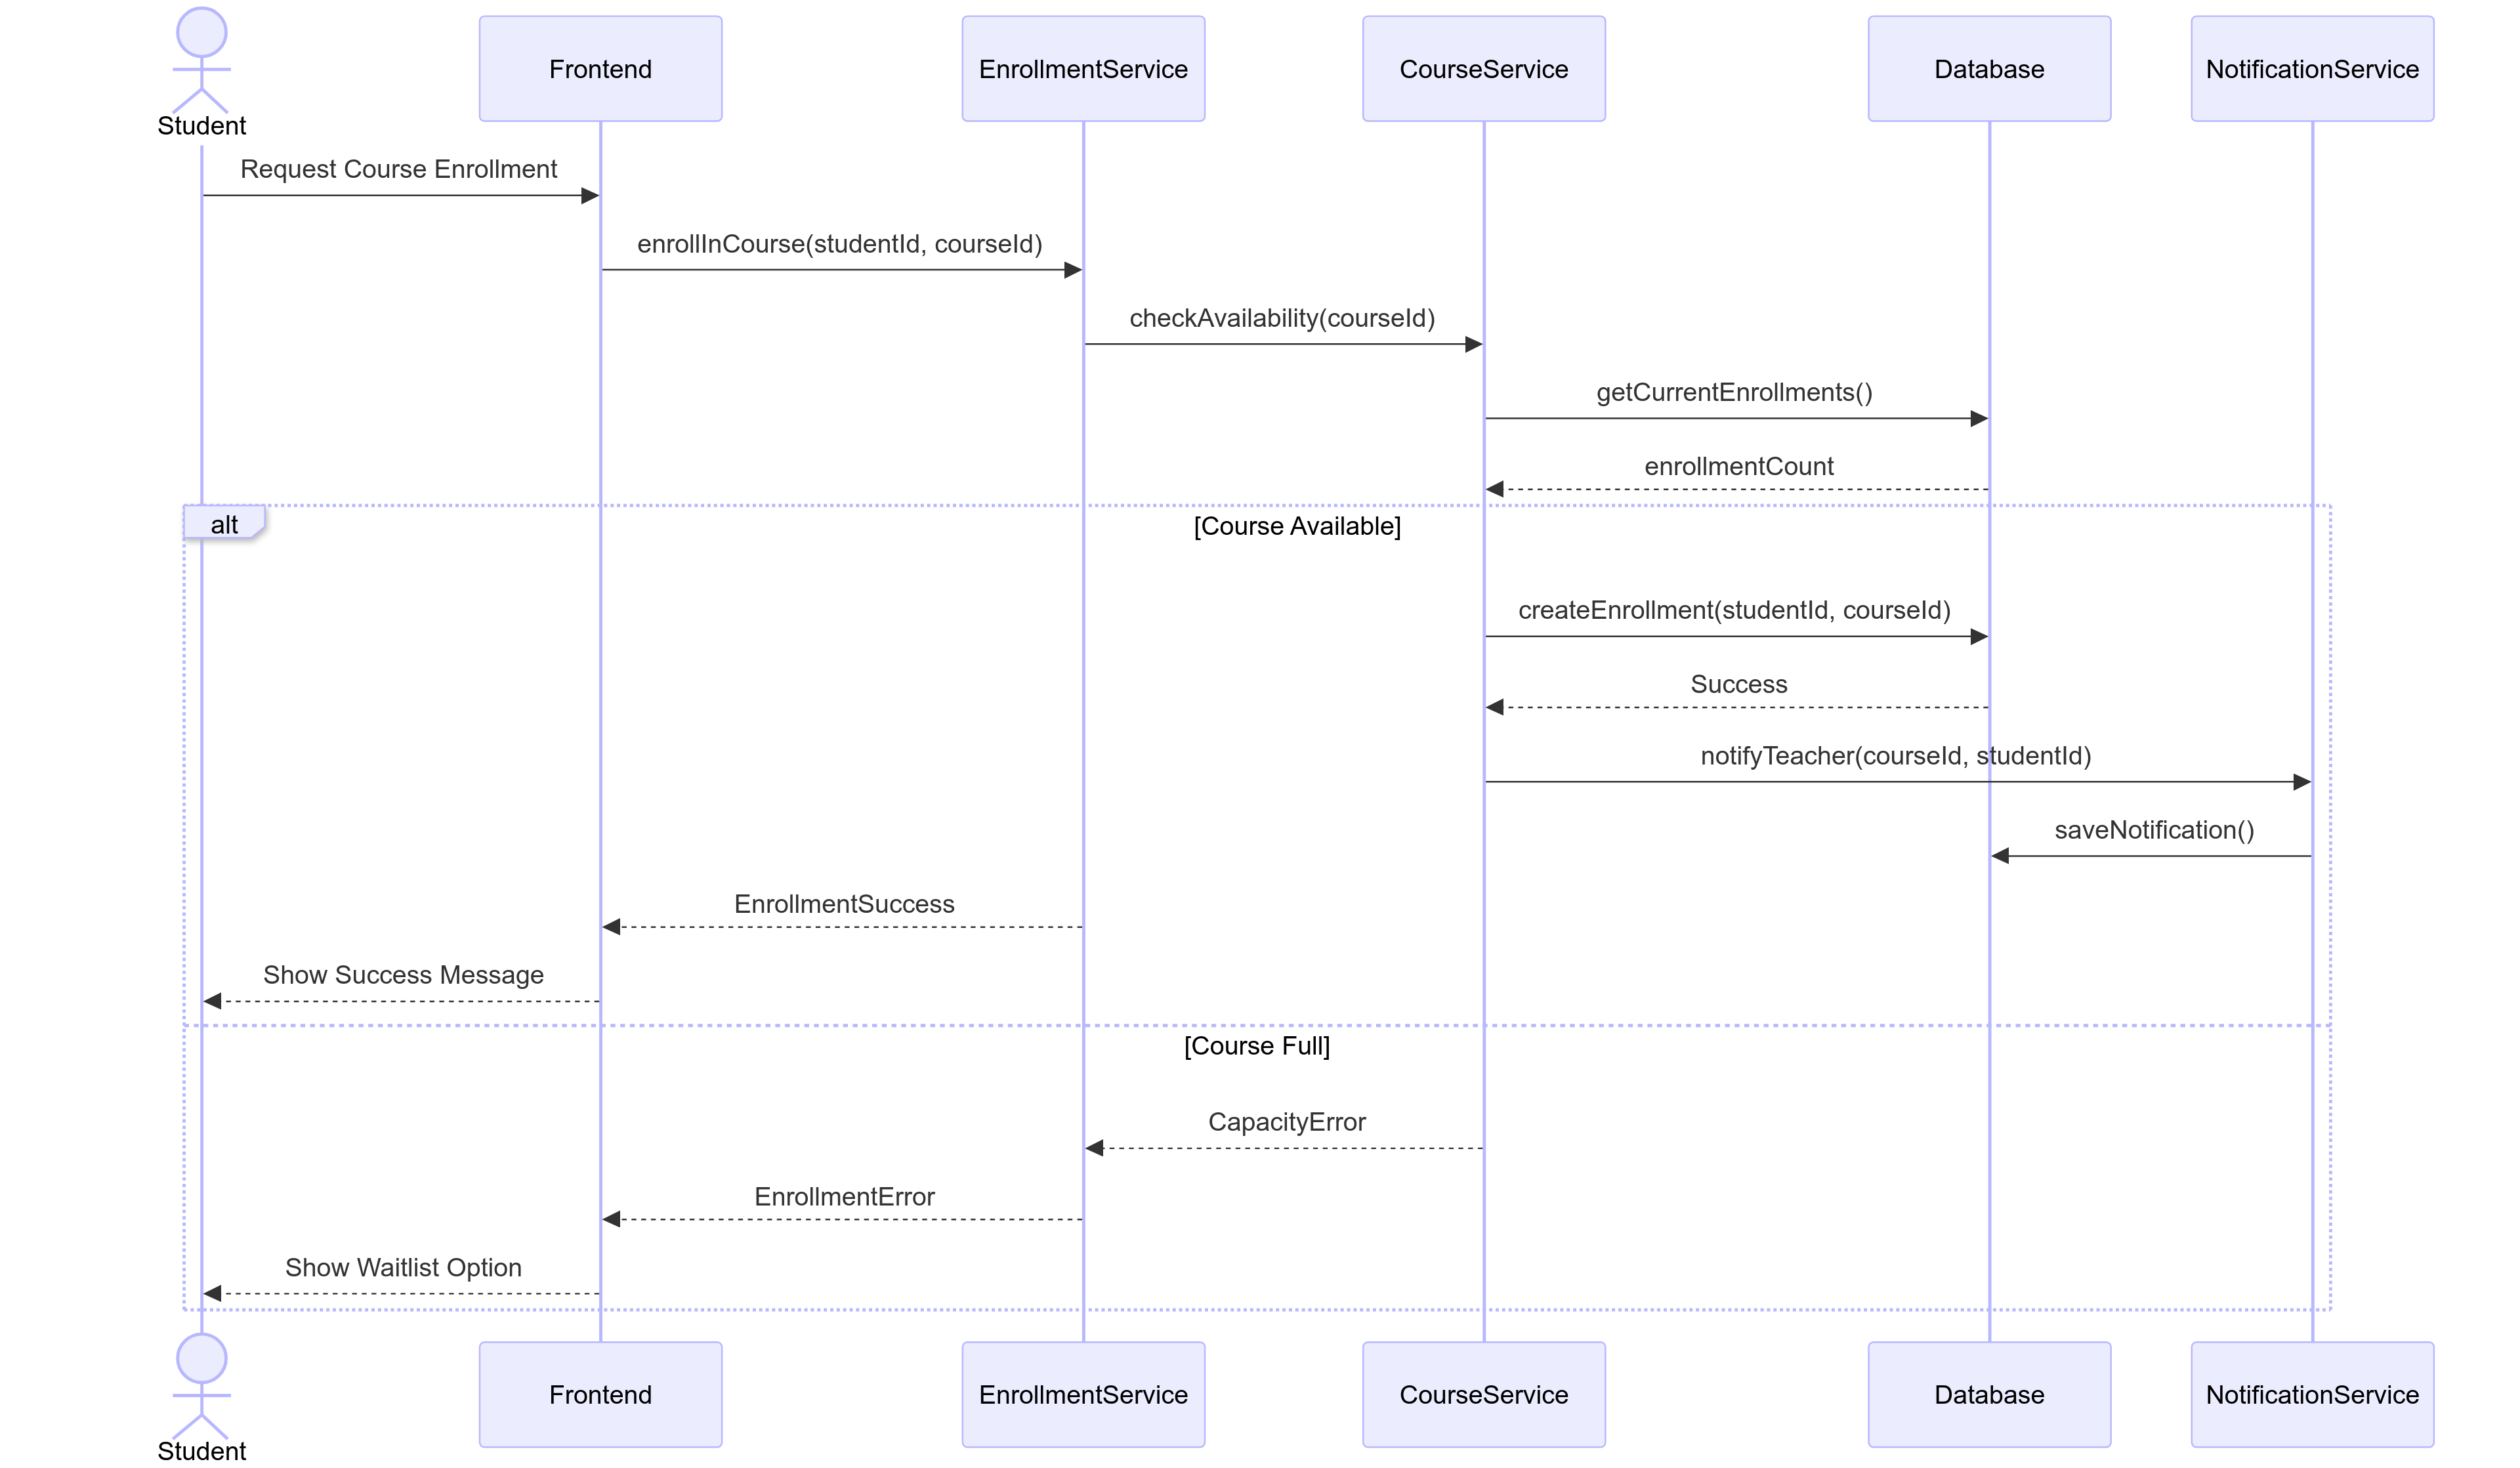
\includegraphics[width=0.9\textwidth,keepaspectratio]{pfe-pics/diagrames/Course Enrollment Process.png}
  \caption{\textbf{Diagramme de flux} pour l'inscription aux cours.}
  \label{fig:course_enrollment}
\end{figure}

Ce diagramme présente :

\begin{itemize}
  \item La recherche et sélection de cours par l'étudiant
  
  \item La vérification des prérequis et disponibilités
  
  \item Le processus d'approbation si nécessaire
  
  \item La confirmation de l'inscription et l'accès au matériel du cours
\end{itemize}

\subsection{Cas d'utilisation}

Le diagramme des cas d'utilisation offre une vue d'ensemble des fonctionnalités du système par type d'utilisateur :

\begin{figure}[H]
  \centering
  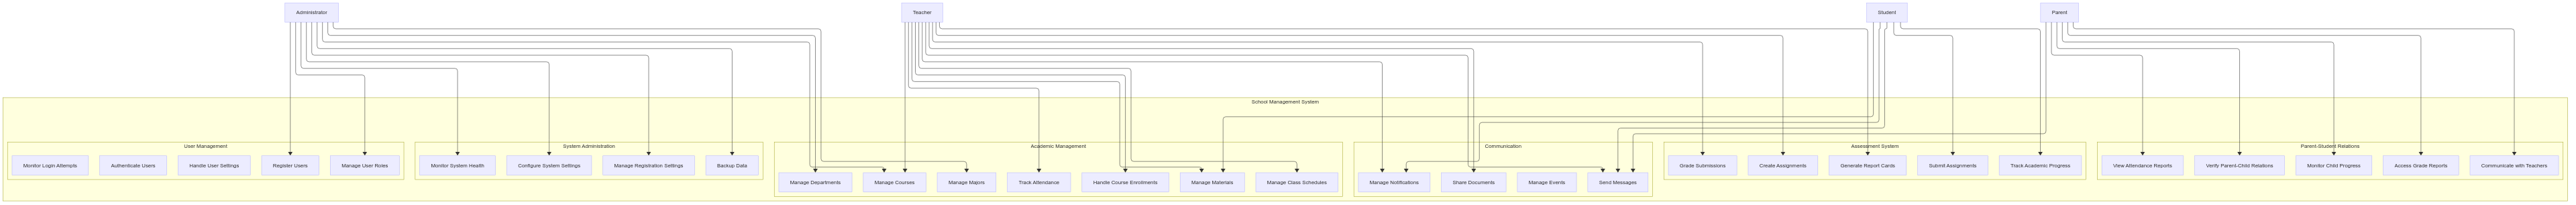
\includegraphics[width=0.9\textwidth,keepaspectratio]{pfe-pics/diagrames/usecase.png}
  \caption{\textbf{Diagramme de cas d'utilisation} du système de gestion scolaire.}
  \label{fig:use_cases}
\end{figure}

Ce diagramme met en évidence :

\begin{itemize}
  \item Les acteurs principaux du système (administrateur, enseignant, étudiant, parent)
  
  \item Les fonctionnalités accessibles à chaque type d'utilisateur
  
  \item Les relations entre les différents cas d'utilisation
  
  \item Les extensions et inclusions entre cas d'utilisation
\end{itemize}

\section{Conception détaillée du système de création de profils IA}

\subsection{Architecture des composants}

L'architecture du système de création de profils IA s'articule autour de plusieurs composants spécialisés :

\begin{figure}[H]
  \centering
  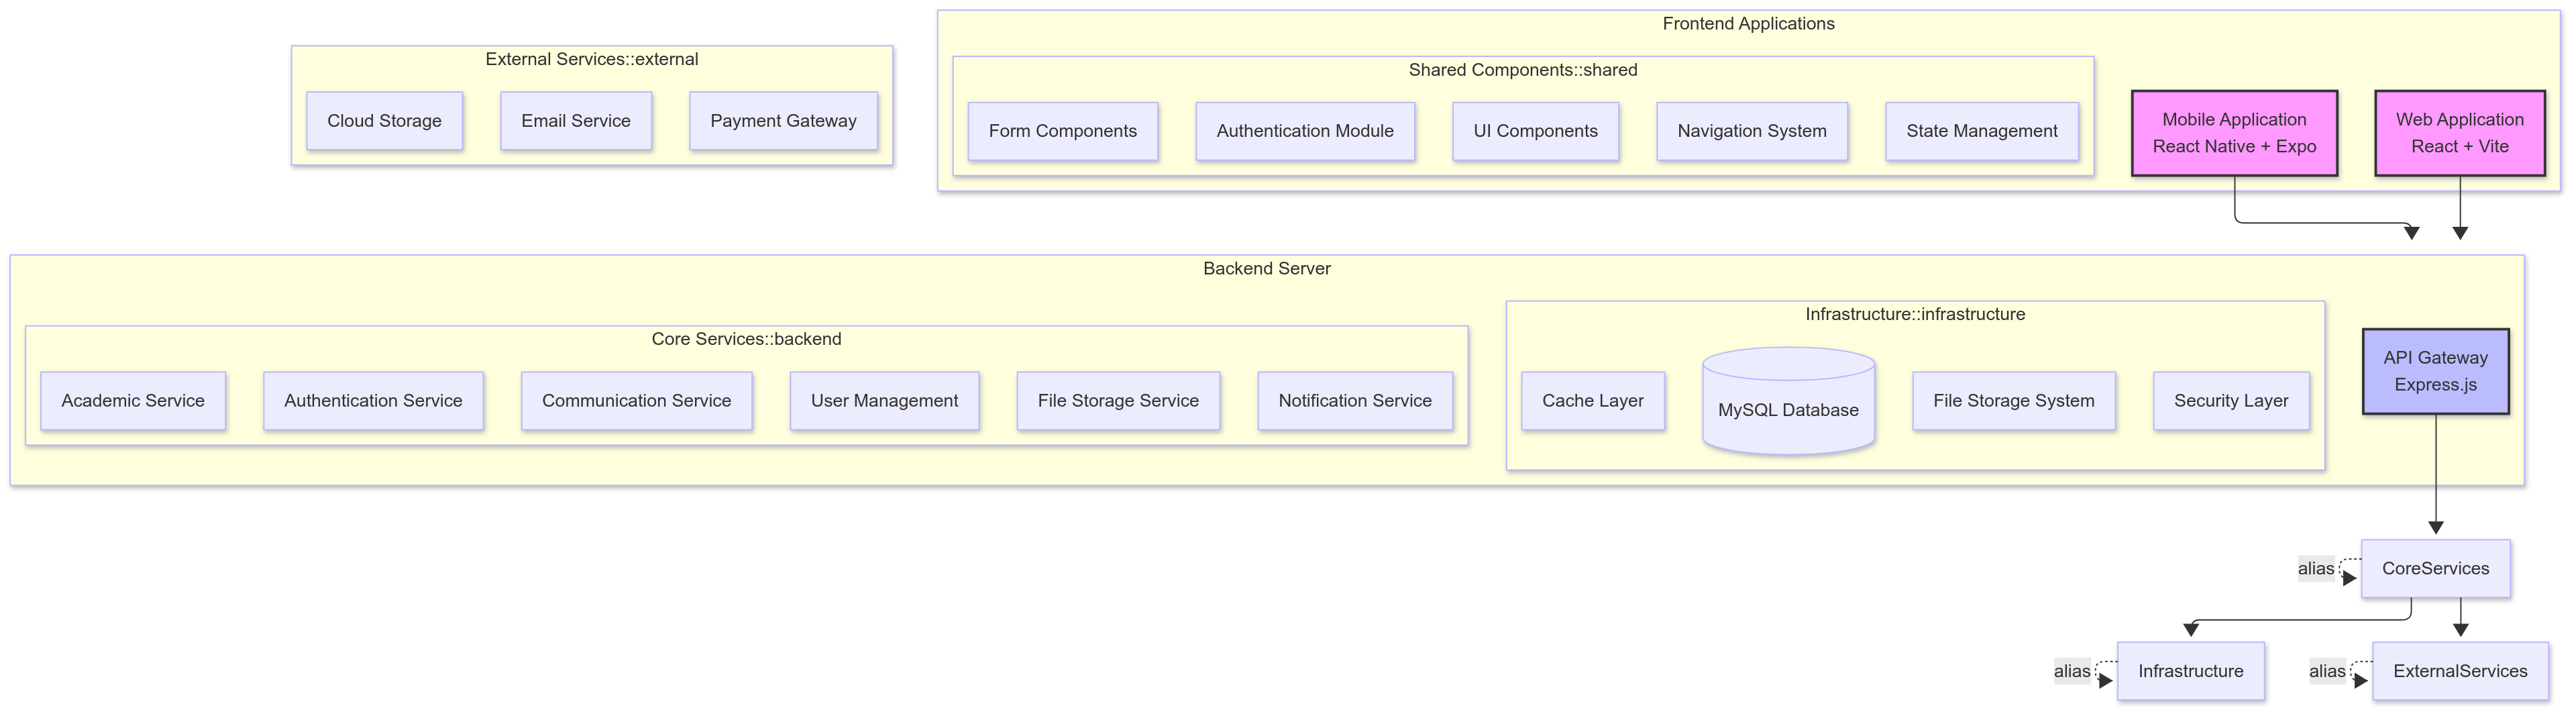
\includegraphics[width=0.9\textwidth,keepaspectratio]{pfe-pics/diagrames/Component Diagram (showing the system_s architecture).png}
  \caption{\textbf{Diagramme de composants} du système de création de profils IA.}
  \label{fig:ai_components}
\end{figure}

Les principaux composants sont :

\begin{itemize}
  \item \textbf{Gestionnaire de profils} : Création et configuration des profils IA
  
  \item \textbf{Processeur de documents} : Traitement et extraction d'informations à partir des documents uploadés
  
  \item \textbf{Moteur d'indexation} : Organisation des connaissances pour une recherche efficace
  
  \item \textbf{Interface conversationnelle} : Gestion des interactions avec les profils IA
  
  \item \textbf{Gestionnaire d'API} : Exposition des fonctionnalités via une API RESTful
  
  \item \textbf{Système d'authentification} : Gestion des utilisateurs et des accès
\end{itemize}

\subsection{Pipeline de traitement des documents}

Le pipeline de traitement des documents constitue un élément central du système de création de profils IA :

\begin{itemize}
  \item \textbf{Étape 1 - Extraction de texte} : Conversion des différents formats de documents en texte brut
  
  \item \textbf{Étape 2 - Analyse structurelle} : Identification des sections, titres, paragraphes et éléments spéciaux
  
  \item \textbf{Étape 3 - Enrichissement sémantique} : Détection des entités, concepts et relations
  
  \item \textbf{Étape 4 - Chunking intelligent} : Segmentation du contenu en unités de connaissance optimales
  
  \item \textbf{Étape 5 - Indexation vectorielle} : Création d'embeddings pour la recherche sémantique
  
  \item \textbf{Étape 6 - Validation et stockage} : Vérification de la qualité et persistance des données traitées
\end{itemize}

\subsection{Modèle de données}

Le modèle de données du système de création de profils IA est conçu pour gérer efficacement les profils, documents et interactions :

\begin{itemize}
  \item \textbf{Profile} : Définition d'un profil IA avec ses paramètres et métadonnées
  
  \item \textbf{Document} : Information sur les documents sources avec leur statut de traitement
  
  \item \textbf{Chunk} : Segments de contenu extraits des documents
  
  \item \textbf{Embedding} : Représentations vectorielles des chunks pour la recherche sémantique
  
  \item \textbf{Conversation} : Sessions de discussion avec un profil IA
  
  \item \textbf{Message} : Échanges individuels au sein d'une conversation
  
  \item \textbf{ApiKey} : Clés d'accès pour l'intégration externe
  
  \item \textbf{User} : Utilisateurs du système avec leurs permissions
\end{itemize}

\subsection{Flux de traitement des requêtes}

Le traitement d'une requête adressée à un profil IA suit un flux optimisé :

\begin{itemize}
  \item \textbf{Réception de la requête} : Validation et prétraitement de la question utilisateur
  
  \item \textbf{Recherche sémantique} : Identification des chunks les plus pertinents dans la base de connaissances
  
  \item \textbf{Construction du contexte} : Assemblage des informations pertinentes avec l'historique de conversation
  
  \item \textbf{Génération de réponse} : Utilisation du modèle d'IA avec le contexte pour produire une réponse
  
  \item \textbf{Post-traitement} : Formatage, vérification et enrichissement de la réponse
  
  \item \textbf{Enregistrement} : Sauvegarde de l'échange pour référence future et amélioration
\end{itemize}

\subsection{Intégration avec les services externes}

Le système s'intègre avec plusieurs services externes pour optimiser ses fonctionnalités :

\begin{itemize}
  \item \textbf{OpenRouter API} : Accès à différents modèles de langage pour la génération de réponses
  
  \item \textbf{Services de stockage objet} : Stockage efficace des documents originaux et traités
  
  \item \textbf{Services d'OCR} : Extraction de texte à partir d'images et documents scannés
  
  \item \textbf{Services d'authentification} : Intégration possible avec des fournisseurs d'identité externes
\end{itemize}

\section{Intégration des deux systèmes}

\subsection{Points d'intégration}

L'intégration entre le système de gestion scolaire et le système de création de profils IA s'effectue à plusieurs niveaux :

\begin{itemize}
  \item \textbf{Authentification unifiée} : Système SSO permettant une navigation fluide entre les deux plateformes
  
  \item \textbf{Association profils-cours} : Possibilité d'associer des profils IA spécifiques à des cours
  
  \item \textbf{Partage de ressources} : Utilisation des documents pédagogiques du système scolaire comme source pour les profils IA
  
  \item \textbf{Intégration UI} : Widgets permettant d'interagir avec les profils IA directement depuis l'interface du système scolaire
\end{itemize}

\subsection{Architecture d'intégration}

L'architecture d'intégration repose sur une approche API-first :

\begin{itemize}
  \item \textbf{API Gateway} : Point d'entrée unifié gérant le routage vers les services appropriés
  
  \item \textbf{Services d'identité partagés} : Gestion centralisée des utilisateurs et autorisations
  
  \item \textbf{Bus d'événements} : Communication asynchrone entre les systèmes pour les mises à jour et notifications
  
  \item \textbf{Cache distribué} : Optimisation des performances pour les données fréquemment accédées
\end{itemize}

\begin{figure}[H]
  \centering
  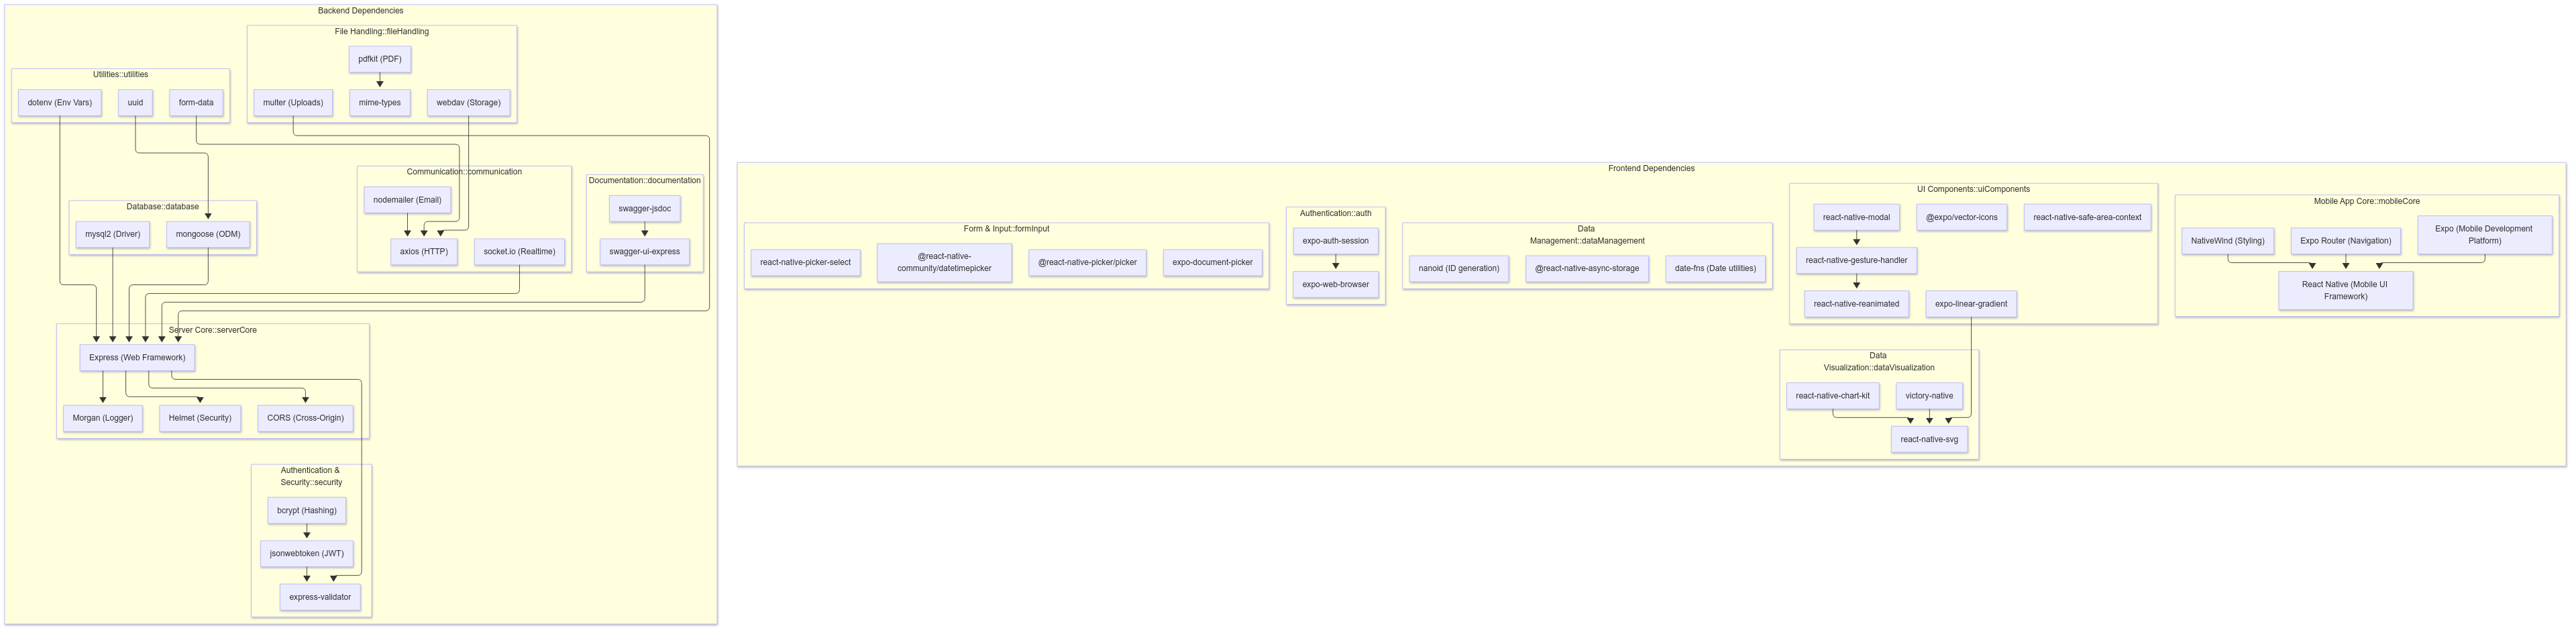
\includegraphics[width=0.9\textwidth,keepaspectratio]{pfe-pics/diagrames/dependeces.png}
  \caption{\textbf{Diagramme de dépendances} montrant l'intégration des systèmes.}
  \label{fig:integration_dependencies}
\end{figure}

\section{Considérations de sécurité et performance}

\subsection{Stratégie de sécurité}

La sécurité a été intégrée à tous les niveaux de la conception :

\begin{itemize}
  \item \textbf{Authentification robuste} : Mécanismes d'authentification modernes avec support MFA
  
  \item \textbf{Autorisation fine} : Contrôle d'accès basé sur les rôles et les ressources
  
  \item \textbf{Protection des données} : Chiffrement des données sensibles au repos et en transit
  
  \item \textbf{Validation des entrées} : Filtrage et validation de toutes les entrées utilisateur
  
  \item \textbf{Audit et journalisation} : Traçabilité des actions sensibles pour détection d'anomalies
  
  \item \textbf{Protection contre les attaques courantes} : Mesures contre XSS, CSRF, injection SQL, etc.
\end{itemize}

\subsection{Optimisation des performances}

Plusieurs stratégies ont été adoptées pour garantir des performances optimales :

\begin{itemize}
  \item \textbf{Mise en cache multicouche} : Cache au niveau du navigateur, de l'API et de la base de données
  
  \item \textbf{Traitement asynchrone} : Utilisation de files d'attente pour les opérations longues
  
  \item \textbf{Pagination et chargement différé} : Optimisation du chargement des données volumineuses
  
  \item \textbf{Optimisation des requêtes} : Indexation et requêtes efficientes sur la base de données
  
  \item \textbf{Distribution de charge} : Répartition du trafic entre plusieurs instances de service
\end{itemize}

\subsection{Stratégie de déploiement}

L'architecture a été conçue pour faciliter un déploiement flexible et évolutif :

\begin{itemize}
  \item \textbf{Conteneurisation} : Packaging des services dans des conteneurs Docker pour portabilité
  
  \item \textbf{Configuration externalisée} : Séparation du code et de la configuration pour adaptation à différents environnements
  
  \item \textbf{Déploiement progressif} : Stratégies de déploiement bleu-vert ou canary pour minimiser les risques
  
  \item \textbf{Surveillance intégrée} : Métriques et alertes pour suivre la santé et les performances du système
\end{itemize}

\section{Gestion de projet}

La réalisation de nos deux systèmes complémentaires a nécessité une planification rigoureuse et une gestion de projet structurée pour garantir l'atteinte des objectifs dans les délais impartis.

\subsection{Approche méthodologique}

Notre approche de gestion de projet s'est appuyée sur une méthodologie hybride combinant :

\begin{itemize}
  \item \textbf{Éléments Agile} : Développement itératif, sessions de revue régulières, adaptation aux retours utilisateurs
  
  \item \textbf{Planification structurée} : Définition claire des jalons et livrables, allocation des ressources
  
  \item \textbf{Gestion des risques} : Identification précoce et stratégies d'atténuation des risques potentiels
\end{itemize}

Cette approche nous a permis de maintenir un équilibre entre la rigueur nécessaire pour un projet académique et la flexibilité requise face aux défis techniques et contraintes temporelles.

\subsection{Organisation temporelle}

Le projet s'est déroulé sur une période de six mois, de novembre 2024 à avril 2025, avec une interruption en fin de période due aux examens nationaux. Le diagramme de Gantt ci-dessous présente la répartition temporelle des différentes phases :

\begin{figure}[H]
  \centering
  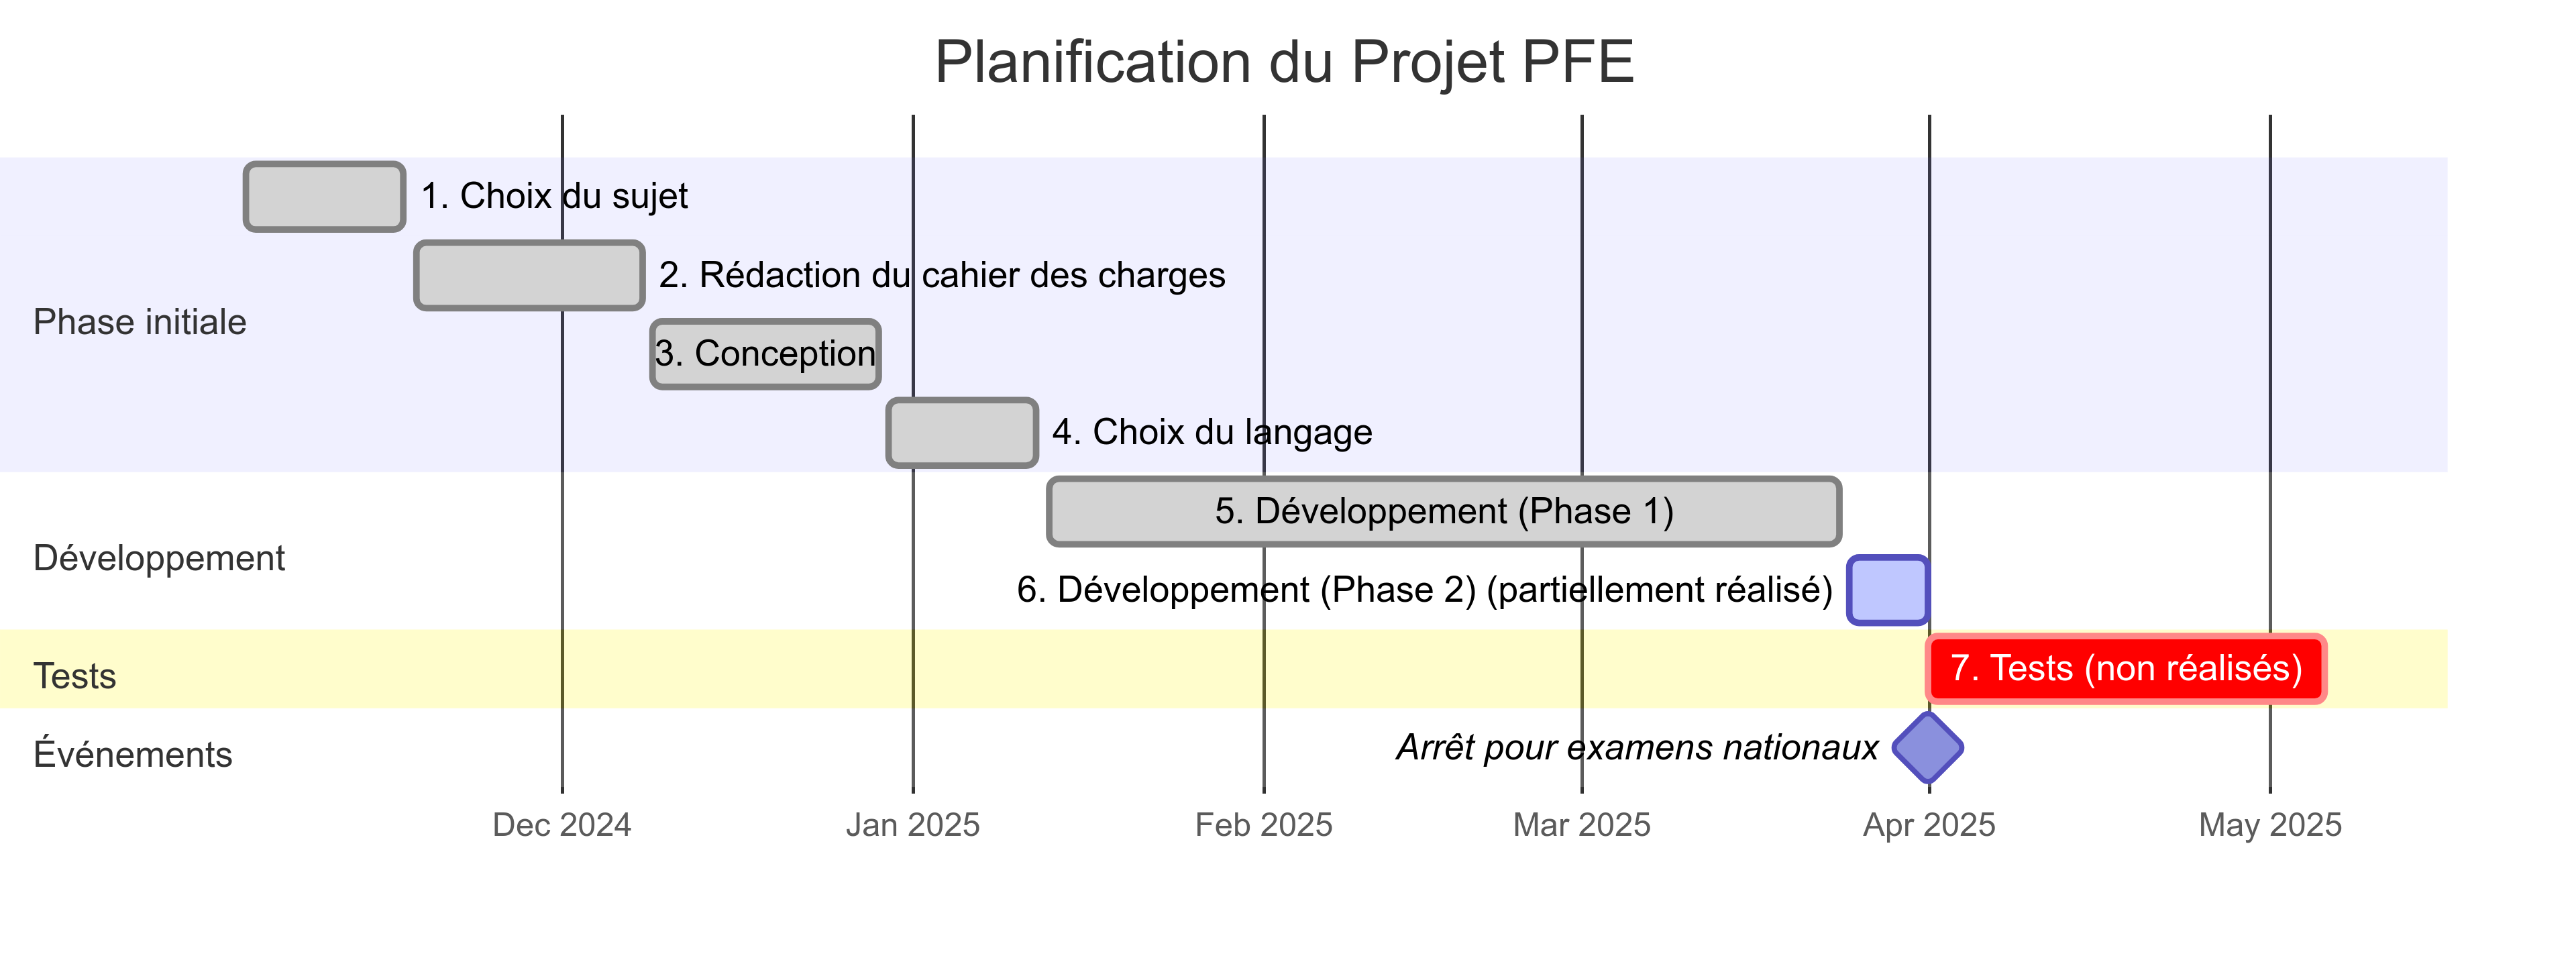
\includegraphics[width=1.0\textwidth,keepaspectratio]{pfe-pics/diagrames/Mermaid Chart - Create complex, visual diagrams with text. A smarter way of creating diagrams.-2025-06-10-203842.png}
  \caption{\textbf{Diagramme de Gantt} montrant la planification temporelle du projet.}
  \label{fig:gantt_chart}
\end{figure}

Les principales phases identifiées sont :

\begin{itemize}
  \item \textbf{Phase d'analyse} (Novembre - Décembre 2024) : Étude des besoins, analyse de l'existant, spécification des exigences
  
  \item \textbf{Phase de conception} (Décembre 2024 - Janvier 2025) : Élaboration des architectures et modèles détaillés
  
  \item \textbf{Phase de développement 1} (Janvier - Février 2025) : Implémentation du système de gestion scolaire
  
  \item \textbf{Phase de développement 2} (Février - Mars 2025) : Implémentation du système de création de profils IA
  
  \item \textbf{Phase d'intégration} (Mars 2025) : Interconnexion des deux systèmes
  
  \item \textbf{Phase de tests et validation} (Mars - début Avril 2025) : Vérification des fonctionnalités et performances
  
  \item \textbf{Phase de documentation} (Avril 2025) : Finalisation de la documentation technique et utilisateur
\end{itemize}

Il est à noter que la phase de développement 2 n'a été que partiellement complétée et que la phase de tests a été limitée en raison des contraintes temporelles liées aux examens nationaux.

\subsection{Dépendances et chemin critique}

Le diagramme PERT ci-dessous illustre les dépendances entre les différentes tâches du projet et met en évidence le chemin critique :

\begin{figure}[H]
  \centering
  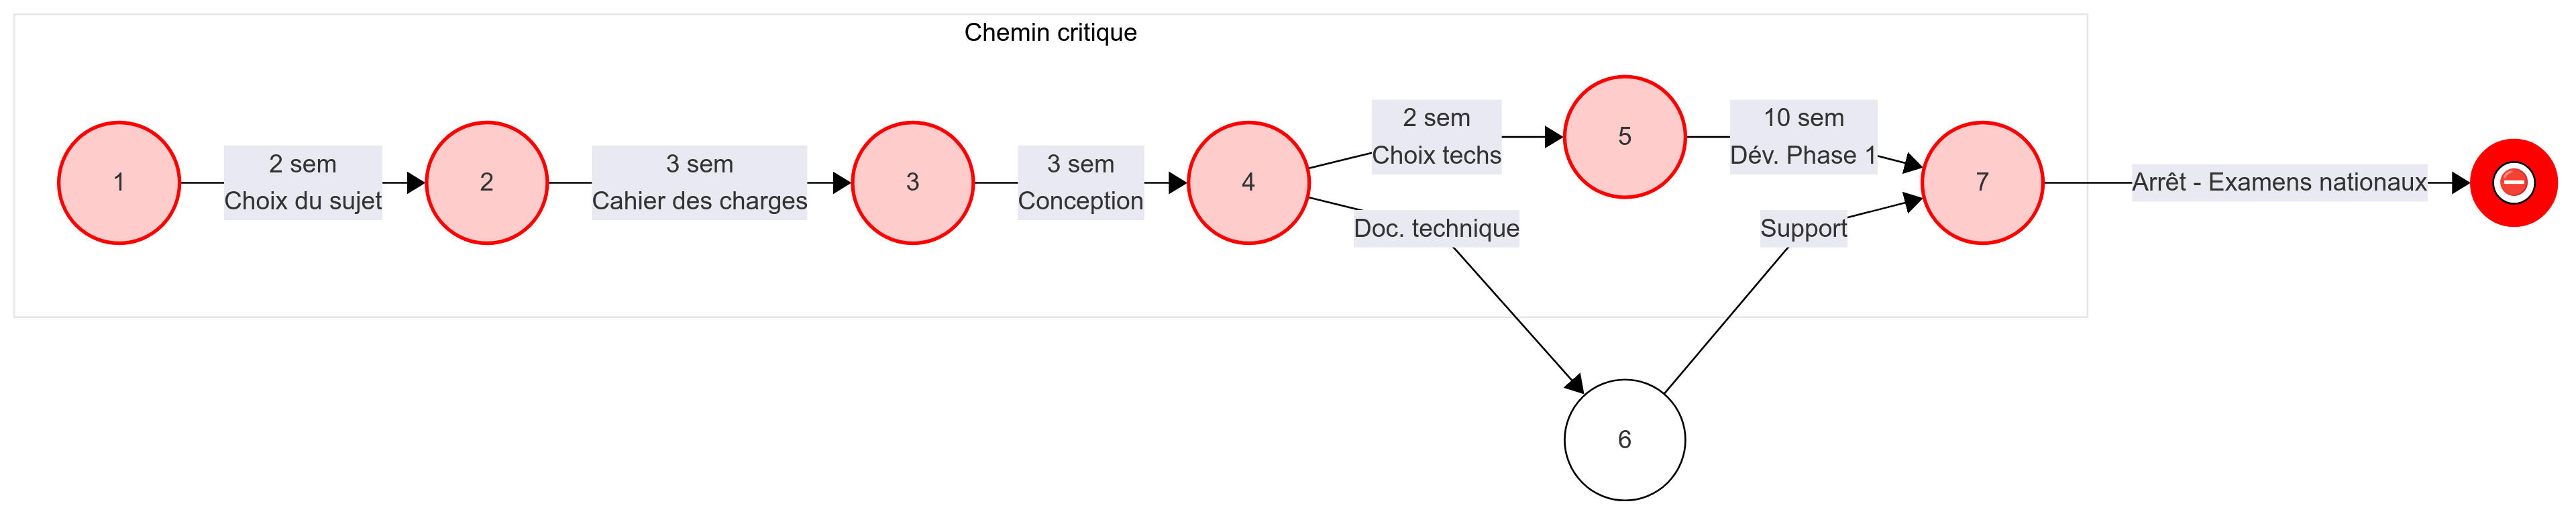
\includegraphics[width=1.0\textwidth,keepaspectratio]{pfe-pics/diagrames/Mermaid Chart - Create complex, visual diagrams with text. A smarter way of creating diagrams.-2025-06-10-203658.png}
  \caption{\textbf{Diagramme PERT} illustrant les dépendances et le chemin critique du projet.}
  \label{fig:pert_diagram}
\end{figure}

Ce diagramme met en évidence :

\begin{itemize}
  \item Les relations de précédence entre les activités
  
  \item Le chemin critique déterminant la durée minimale du projet
  
  \item Les marges disponibles pour certaines activités non critiques
  
  \item Les points de synchronisation nécessaires entre les différents volets du projet
\end{itemize}

L'analyse du chemin critique a révélé que les activités liées à la conception et au développement initial du système de gestion scolaire étaient particulièrement déterminantes pour le respect des délais globaux.

\subsection{Répartition des responsabilités}

Le projet a été mené par une équipe de deux étudiants, avec une répartition des responsabilités basée sur les compétences et centres d'intérêt de chacun :

\begin{itemize}
  \item \textbf{Développement frontend} : Conception et implémentation des interfaces web et mobile
  
  \item \textbf{Développement backend} : Architecture serveur, API et logique métier
  
  \item \textbf{Intégration IA} : Conception et développement du système de création de profils IA
  
  \item \textbf{Base de données} : Modélisation et optimisation des schémas de données
  
  \item \textbf{Tests et validation} : Élaboration et exécution des plans de test
  
  \item \textbf{Documentation} : Rédaction de la documentation technique et utilisateur
\end{itemize}

Cette organisation a permis une progression parallèle sur plusieurs fronts tout en maintenant une cohérence globale grâce à des points de synchronisation réguliers.

\subsection{Gestion des risques}

Une analyse des risques a été réalisée en début de projet, identifiant plusieurs facteurs potentiels d'échec et leurs stratégies d'atténuation :

\begin{itemize}
  \item \textbf{Risque technique} : Complexité de l'intégration IA → Approche progressive avec prototypes
  
  \item \textbf{Risque temporel} : Contraintes liées aux examens → Priorisation des fonctionnalités essentielles
  
  \item \textbf{Risque de coordination} : Communication d'équipe → Outils collaboratifs et réunions régulières
  
  \item \textbf{Risque de périmètre} : Dérive fonctionnelle → Définition claire du MVP et gestion stricte du scope
\end{itemize}

Cette gestion proactive des risques a contribué à maintenir le projet sur les rails malgré plusieurs défis rencontrés en cours de route.

\subsection{Outils de gestion de projet}

Plusieurs outils ont été utilisés pour faciliter la coordination et le suivi du projet :

\begin{itemize}
  \item \textbf{Gestion des tâches} : Trello pour la visualisation des sprints et du backlog
  
  \item \textbf{Gestion du code source} : GitHub avec workflow d'intégration continue
  
  \item \textbf{Communication} : Discord pour les échanges quotidiens et sessions de travail
  
  \item \textbf{Documentation} : Notion pour la documentation évolutive et le partage de ressources
  
  \item \textbf{Suivi du temps} : Toggl pour mesurer l'effort consacré aux différentes tâches
\end{itemize}

Ces outils ont permis de maintenir une visibilité sur l'avancement du projet et de faciliter la collaboration malgré les contraintes de travail à distance.

\section{Conclusion de la conception}

La conception détaillée présentée dans ce chapitre établit une base solide pour l'implémentation de nos deux systèmes complémentaires. L'approche architecturale adoptée privilégie :

\begin{itemize}
  \item La modularité et l'extensibilité pour faciliter l'évolution future
  
  \item La séparation claire des responsabilités pour une maintenance simplifiée
  
  \item L'intégration harmonieuse des deux systèmes pour une expérience utilisateur cohérente
  
  \item La sécurité et la performance comme préoccupations transversales
\end{itemize}

Les diagrammes et modèles élaborés serviront de guide pour la phase d'implémentation, tout en laissant la flexibilité nécessaire pour s'adapter aux défis techniques qui pourraient survenir durant le développement.

L'architecture proposée répond aux exigences fonctionnelles et non fonctionnelles identifiées dans le cahier des charges, et pose les fondations pour des systèmes robustes, évolutifs et centrés sur l'utilisateur. 
\chapter*{Chapitre 3 : Réalisation et mise en œuvre des systèmes}
\addcontentsline{toc}{chapter}{Chapitre 3 : Réalisation et mise en œuvre des systèmes}
\thispagestyle{fancy}
\setcounter{section}{0}
\newpage

\section{Outils et technologies de développement}
Pour la réalisation de nos deux projets complémentaires, nous avons sélectionné un ensemble d'outils et de technologies modernes qui répondent aux exigences de performance, de scalabilité et de maintenabilité.

\subsection{Environnement de développement}
L'environnement de développement a été configuré avec soin pour assurer une productivité optimale et une collaboration efficace :

\begin{itemize}
  \item \textbf{Visual Studio Code} : Comme éditeur de code principal avec des extensions pour TypeScript, React, Python et ESLint
  
  \item \textbf{Git et GitHub} : Pour la gestion de versions et la collaboration entre les membres de l'équipe
  
  \item \textbf{Docker} : Pour la conteneurisation des services et la cohérence des environnements de développement
  
  \item \textbf{Postman} : Pour tester et documenter les API REST
  
  \item \textbf{Chrome DevTools} : Pour le débogage et l'optimisation des performances frontend
  
  \item \textbf{MongoDB Compass et pgAdmin} : Pour la gestion visuelle des bases de données
\end{itemize}

\subsection{Technologies frontend}
Pour le développement des interfaces utilisateur, nous avons adopté des technologies modernes et performantes :

\subsubsection{Système de gestion scolaire}

\begin{itemize}
  \item \textbf{React 19} : Bibliothèque JavaScript pour la construction d'interfaces utilisateur réactives
  
  \item \textbf{TypeScript} : Langage typé apportant robustesse et maintenabilité au code
  
  \item \textbf{Vite} : Outil de build rapide pour le développement et la production
  
  \item \textbf{Tailwind CSS} : Framework CSS utilitaire pour un design responsive et personnalisable
  
  \item \textbf{React Router} : Pour la gestion du routage et de la navigation
  
  \item \textbf{React Hook Form} : Pour la gestion efficace des formulaires avec validation
  
  \item \textbf{Radix UI} : Composants UI accessibles et personnalisables
  
  \item \textbf{React Query} : Pour la gestion optimisée des requêtes API et du cache
  
  \item \textbf{React Native} : Pour le développement des applications mobiles multiplateformes
  
  \item \textbf{Expo} : Plateforme simplifiant le développement React Native
\end{itemize}

\subsubsection{Système de création de profils IA}

\begin{itemize}
  \item \textbf{React} : Pour la construction de l'interface utilisateur
  
  \item \textbf{TypeScript} : Pour un code plus robuste et maintenable
  
  \item \textbf{Chakra UI} : Bibliothèque de composants accessibles et esthétiques
  
  \item \textbf{Tailwind CSS} : Pour la stylisation efficace des composants
  
  \item \textbf{React Router} : Pour la navigation entre les différentes vues
  
  \item \textbf{React Query} : Pour la gestion optimisée des requêtes API
  
  \item \textbf{Framer Motion} : Pour les animations et transitions fluides
\end{itemize}

\subsection{Technologies backend}

Les backends de nos deux systèmes ont été développés avec des technologies adaptées à leurs besoins spécifiques :

\subsubsection{Système de gestion scolaire}

\begin{itemize}
  \item \textbf{Node.js} : Environnement d'exécution JavaScript côté serveur
  
  \item \textbf{Express} : Framework web minimaliste et flexible pour Node.js
  
  \item \textbf{TypeScript} : Pour un développement backend typé et robuste
  
  \item \textbf{MySQL} : Système de gestion de base de données relationnelle
  
  \item \textbf{Mongoose} : ODM pour l'intégration avec MongoDB (pour certaines fonctionnalités spécifiques)
  
  \item \textbf{JWT} : Pour l'authentification et la gestion des sessions
  
  \item \textbf{Multer} : Pour la gestion des uploads de fichiers
  
  \item \textbf{Socket.IO} : Pour les fonctionnalités en temps réel
  
  \item \textbf{Swagger} : Pour la documentation automatique des API
\end{itemize}

\subsubsection{Système de création de profils IA}

\begin{itemize}
  \item \textbf{FastAPI} : Framework Python moderne, performant et facile à utiliser
  
  \item \textbf{SQLAlchemy} : ORM Python pour l'interaction avec la base de données
  
  \item \textbf{Pydantic} : Pour la validation des données et la sérialisation
  
  \item \textbf{PostgreSQL} : Base de données relationnelle robuste
  
  \item \textbf{Alembic} : Pour les migrations de base de données
  
  \item \textbf{PyPDF2, python-docx} : Pour le traitement des documents
  
  \item \textbf{OpenAI API} : Pour l'intégration avec les modèles de langage
  
  \item \textbf{Redis} : Pour la mise en cache et la limitation de débit
  
  \item \textbf{Supabase} : Pour l'authentification et le stockage de fichiers
\end{itemize}

\subsection{Outils de déploiement et d'intégration continue}

Pour assurer un processus de développement fluide et des déploiements fiables :

\begin{itemize}
  \item \textbf{Docker et Docker Compose} : Pour la conteneurisation et l'orchestration des services
  
  \item \textbf{GitHub Actions} : Pour l'automatisation des tests et des déploiements
  
  \item \textbf{Nginx} : Comme serveur web et reverse proxy
  
  \item \textbf{PM2} : Pour la gestion des processus Node.js en production
  
  \item \textbf{Gunicorn} : Serveur WSGI pour les applications Python
\end{itemize}

\section{Développement du système de gestion scolaire}

\subsection{Implémentation du backend}
Le développement du backend du système de gestion scolaire a suivi une approche structurée basée sur l'architecture en couches :

\begin{itemize}
  \item \textbf{Structure du projet} : Organisation en modules fonctionnels (utilisateurs, cours, présences, notes, etc.)
  
  \item \textbf{API RESTful} : Conception d'endpoints suivant les bonnes pratiques REST avec des routes clairement définies
  
  \item \textbf{Middleware d'authentification} : Implémentation d'un système robuste basé sur JWT avec différents niveaux d'autorisation
  
  \item \textbf{Validation des données} : Utilisation d'express-validator pour garantir l'intégrité des données entrantes
  
  \item \textbf{Gestion des erreurs} : Mise en place d'un système centralisé de gestion des exceptions
  
  \item \textbf{Documentation API} : Intégration de Swagger pour une documentation interactive et toujours à jour
\end{itemize}

Le code suivant illustre la structure d'un contrôleur typique pour la gestion des cours :

\begin{lstlisting}[style=codestyle, language=JavaScript]
// src/controllers/courseController.ts
import { Request, Response } from 'express';
import { CourseService } from '../services/courseService';
import { handleError } from '../utils/errorHandler';

export class CourseController {
  private courseService: CourseService;
  
  constructor() {
    this.courseService = new CourseService();
  }
  
  public async createCourse(req: Request, res: Response): Promise<void> {
    try {
      const courseData = req.body;
      const teacherId = req.user.id; // From JWT token
      
      const course = await this.courseService.createCourse(courseData, teacherId);
      
      res.status(201).json({
        success: true,
        data: course
      });
    } catch (error) {
      handleError(error, res);
    }
  }
  
  // Other course-related methods...
}
\end{lstlisting}

\subsection{Développement des interfaces web}

Le développement des interfaces web a été réalisé avec une attention particulière à l'expérience utilisateur, en créant des interfaces adaptées à chaque type d'utilisateur du système.

\subsubsection{Interface administrateur}

L'interface administrateur offre une vue complète du système avec des fonctionnalités de gestion avancées :

\begin{figure}[H]
  \centering
  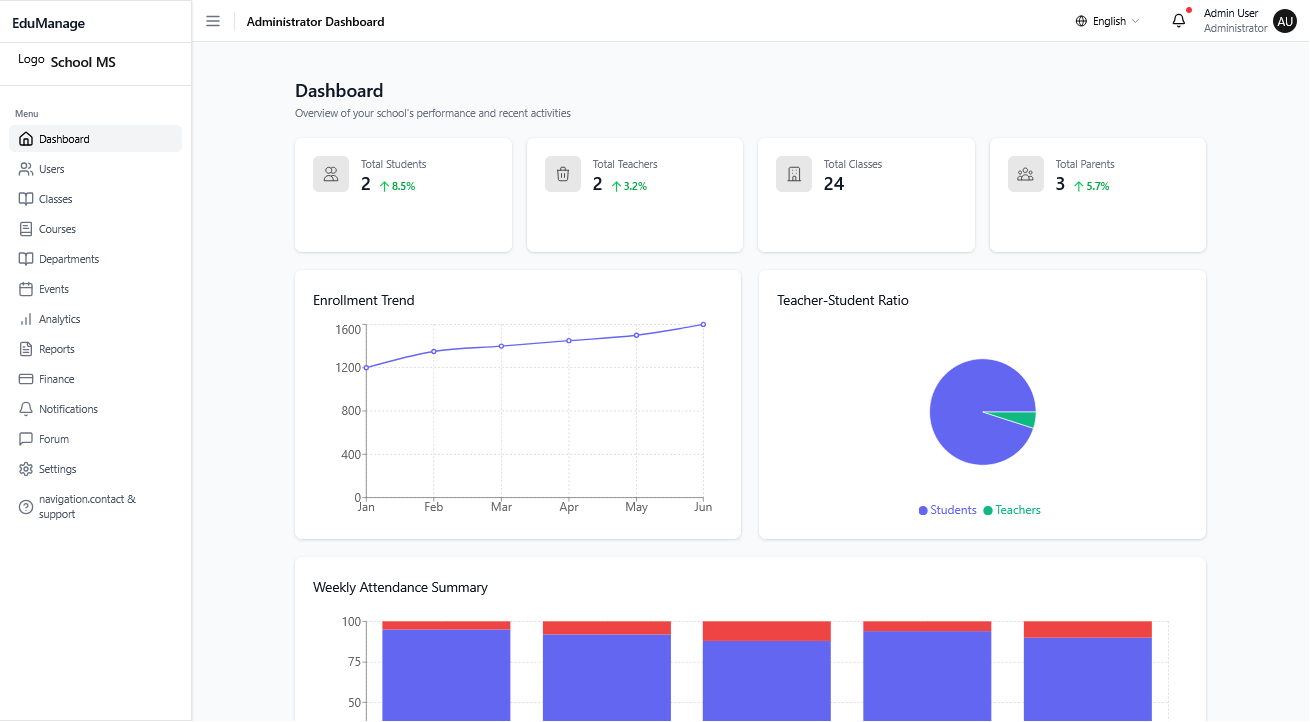
\includegraphics[width=0.85\textwidth,keepaspectratio]{pfe-pics/admin/Screenshot 2025-06-09 at 22-38-06 Vite React TS.png}
  \caption{\textbf{Tableau de bord administrateur} présentant une vue d'ensemble des métriques du système.}
  \label{fig:admin_dashboard}
\end{figure}

Les principales fonctionnalités développées pour l'administrateur comprennent :

\begin{itemize}
  \item \textbf{Tableau de bord analytique} : Visualisation des statistiques clés de l'établissement
  
  \item \textbf{Gestion des utilisateurs} : Interface complète pour créer, modifier et gérer les comptes
  
  \item \textbf{Configuration du système} : Paramètres généraux et personnalisation
  
  \item \textbf{Gestion des cours} : Supervision de tous les cours et programmes
\end{itemize}

\begin{figure}[H]
  \centering
  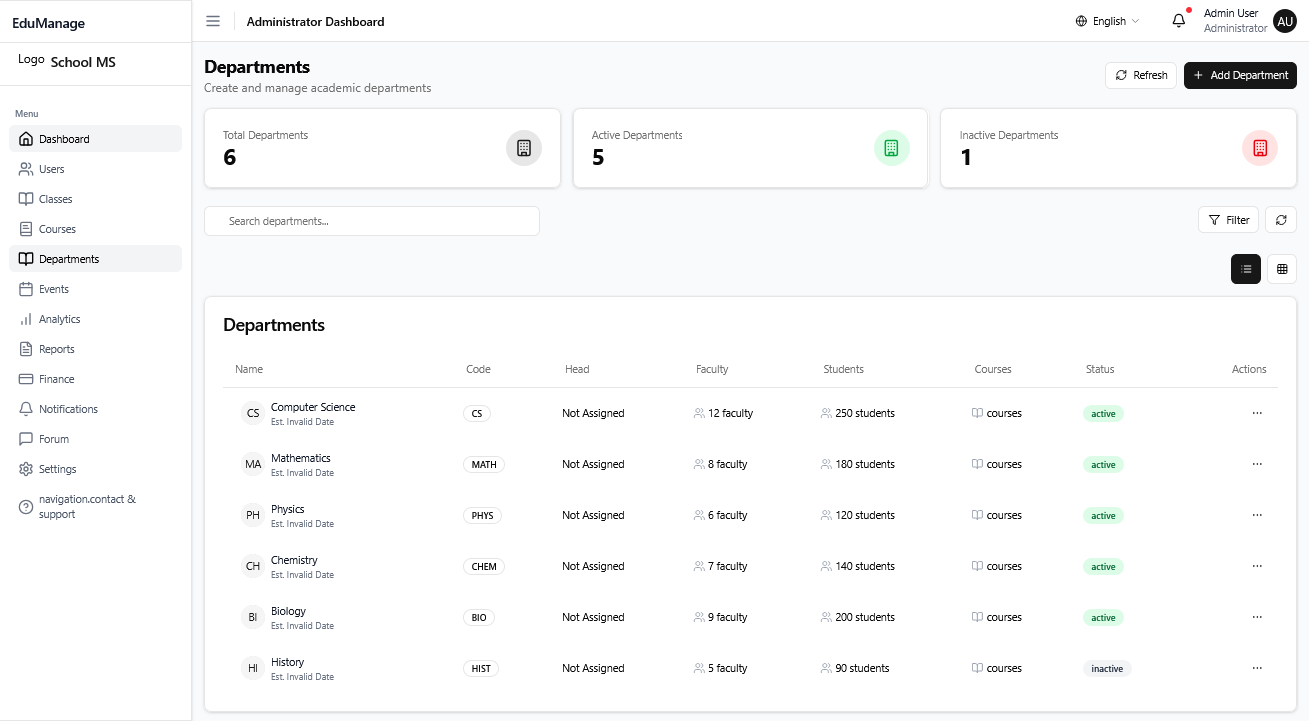
\includegraphics[width=0.85\textwidth,keepaspectratio]{pfe-pics/admin/Screenshot 2025-06-09 at 22-39-15 Vite React TS.png}
  \caption{\textbf{Interface de gestion des utilisateurs} permettant d'administrer les différents types de comptes.}
  \label{fig:user_management}
\end{figure}

\begin{figure}[H]
  \centering
  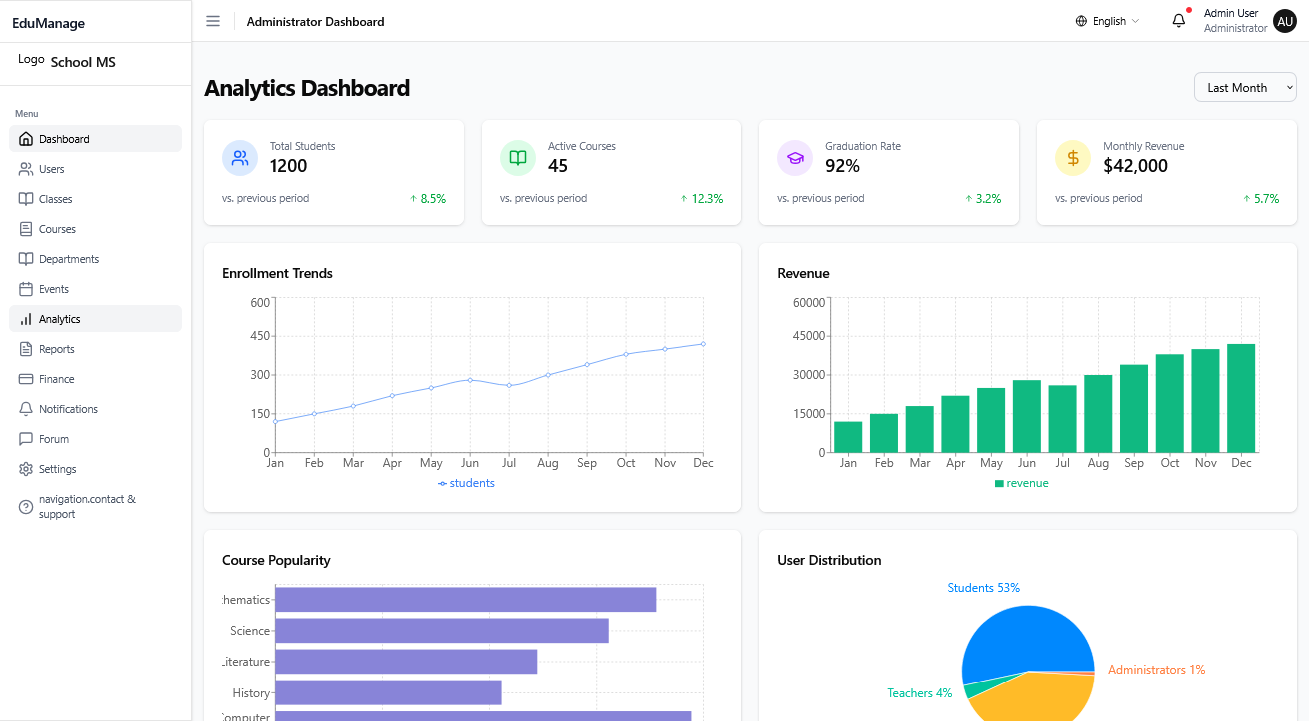
\includegraphics[width=0.85\textwidth,keepaspectratio]{pfe-pics/admin/Screenshot 2025-06-09 at 22-40-11 Vite React TS.png}
  \caption{\textbf{Interface de gestion des cours} avec options de filtrage et d'organisation.}
  \label{fig:course_management_admin}
\end{figure}

\subsubsection{Interface enseignant}

L'interface enseignant a été conçue pour faciliter la gestion pédagogique et le suivi des étudiants :

\begin{figure}[H]
  \centering
  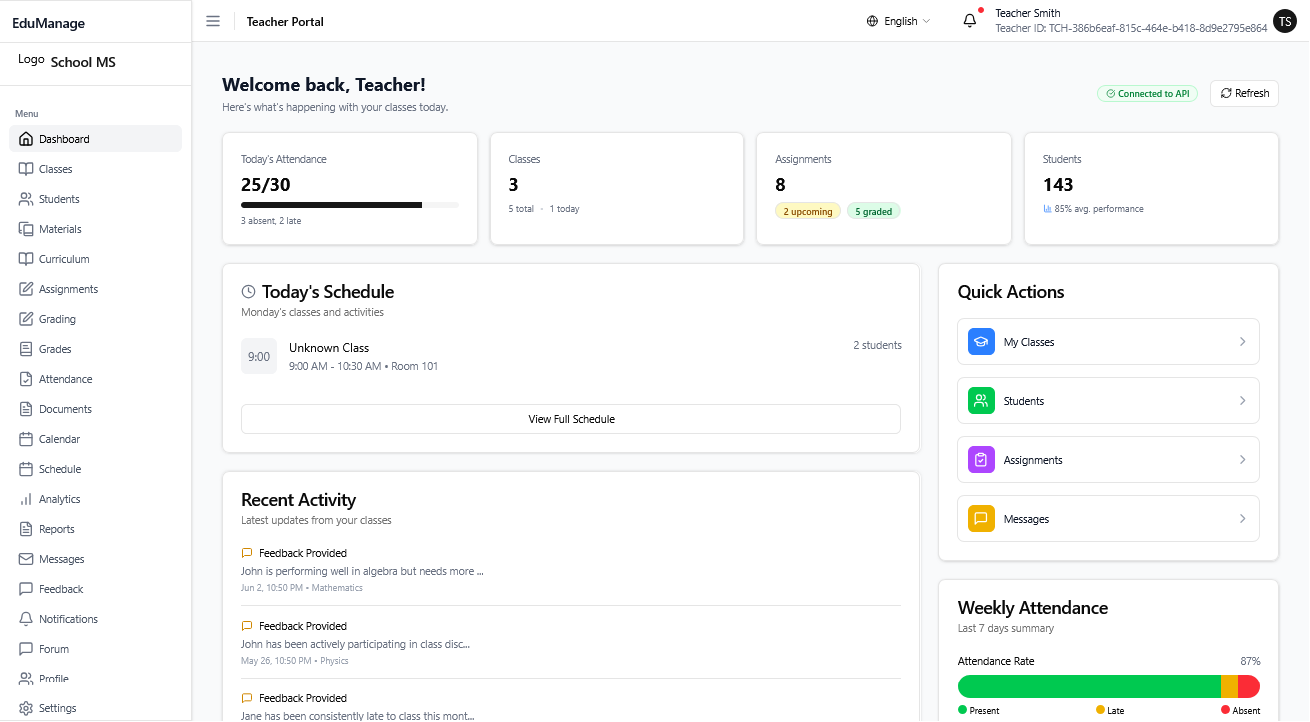
\includegraphics[width=0.85\textwidth,keepaspectratio]{pfe-pics/teacher/Screenshot 2025-06-09 at 22-51-23 Vite React TS.png}
  \caption{\textbf{Tableau de bord enseignant} avec vue d'ensemble des cours et activités récentes.}
  \label{fig:teacher_dashboard}
\end{figure}

Les fonctionnalités clés développées pour les enseignants incluent :

\begin{itemize}
  \item \textbf{Gestion des cours} : Création et organisation du contenu pédagogique
  
  \item \textbf{Suivi des présences} : Interface intuitive pour l'enregistrement des présences
  
  \item \textbf{Évaluation} : Système complet pour la création, notation et commentaire des travaux
  
  \item \textbf{Communication} : Outils pour interagir avec les étudiants et les parents
\end{itemize}

\begin{figure}[H]
  \centering
  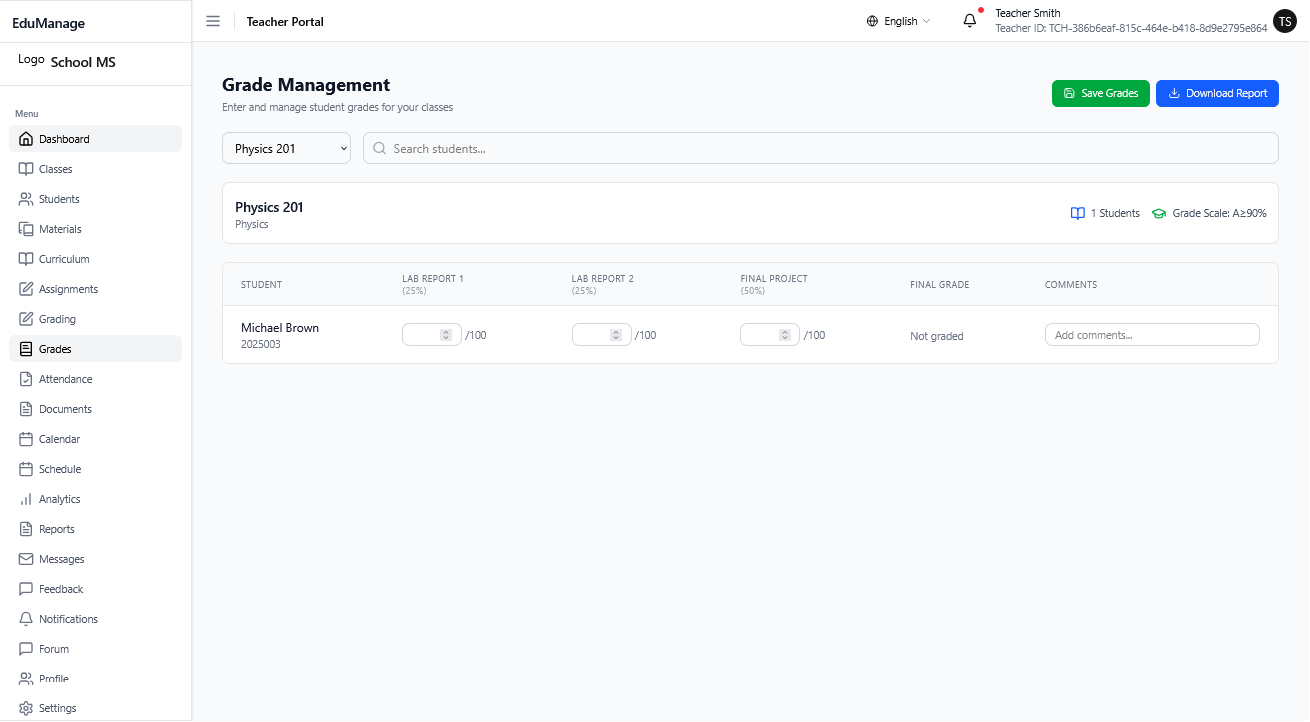
\includegraphics[width=0.85\textwidth,keepaspectratio]{pfe-pics/teacher/Screenshot 2025-06-09 at 22-53-59 Vite React TS.png}
  \caption{\textbf{Interface de prise de présence} permettant un enregistrement rapide et efficace.}
  \label{fig:attendance_taking}
\end{figure}

\begin{figure}[H]
  \centering
  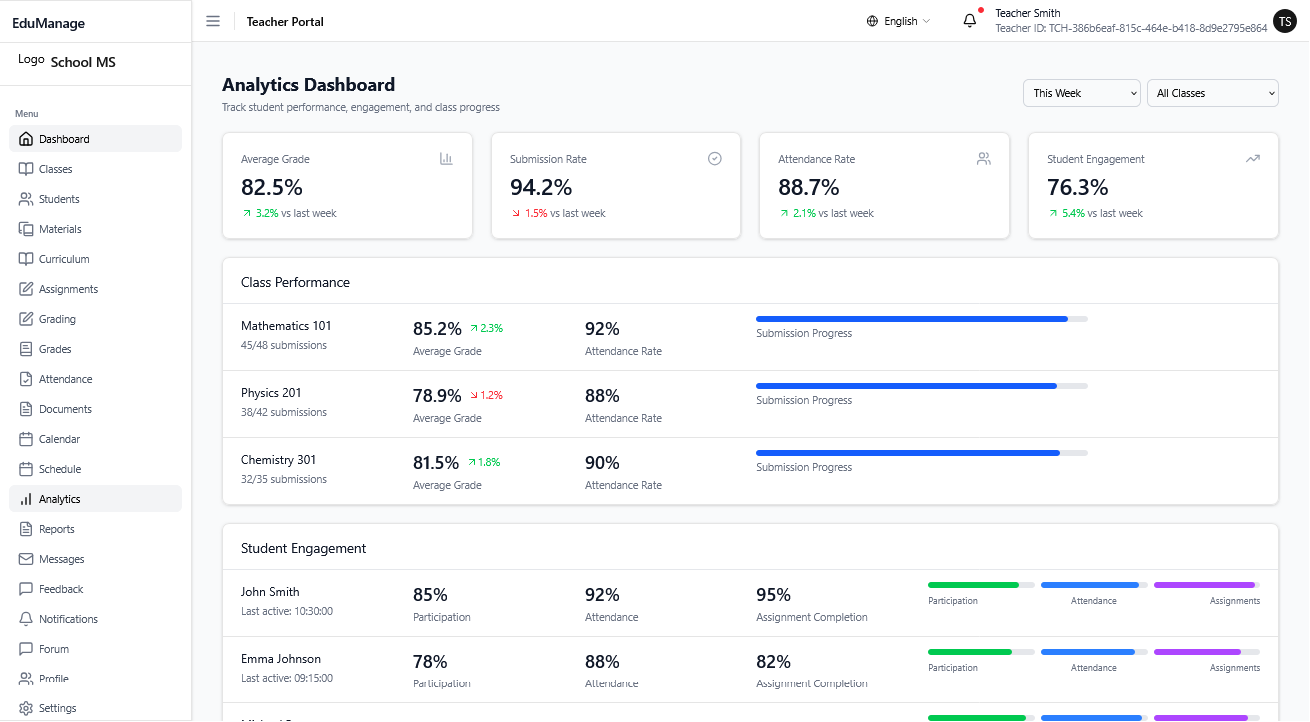
\includegraphics[width=0.85\textwidth,keepaspectratio]{pfe-pics/teacher/Screenshot 2025-06-09 at 22-55-38 Vite React TS.png}
  \caption{\textbf{Interface de notation} avec options de feedback détaillé pour les étudiants.}
  \label{fig:grading_interface}
\end{figure}

\subsubsection{Interface étudiant}

L'interface étudiant a été développée pour offrir un accès clair aux cours, devoirs et résultats :

\begin{figure}[H]
  \centering
  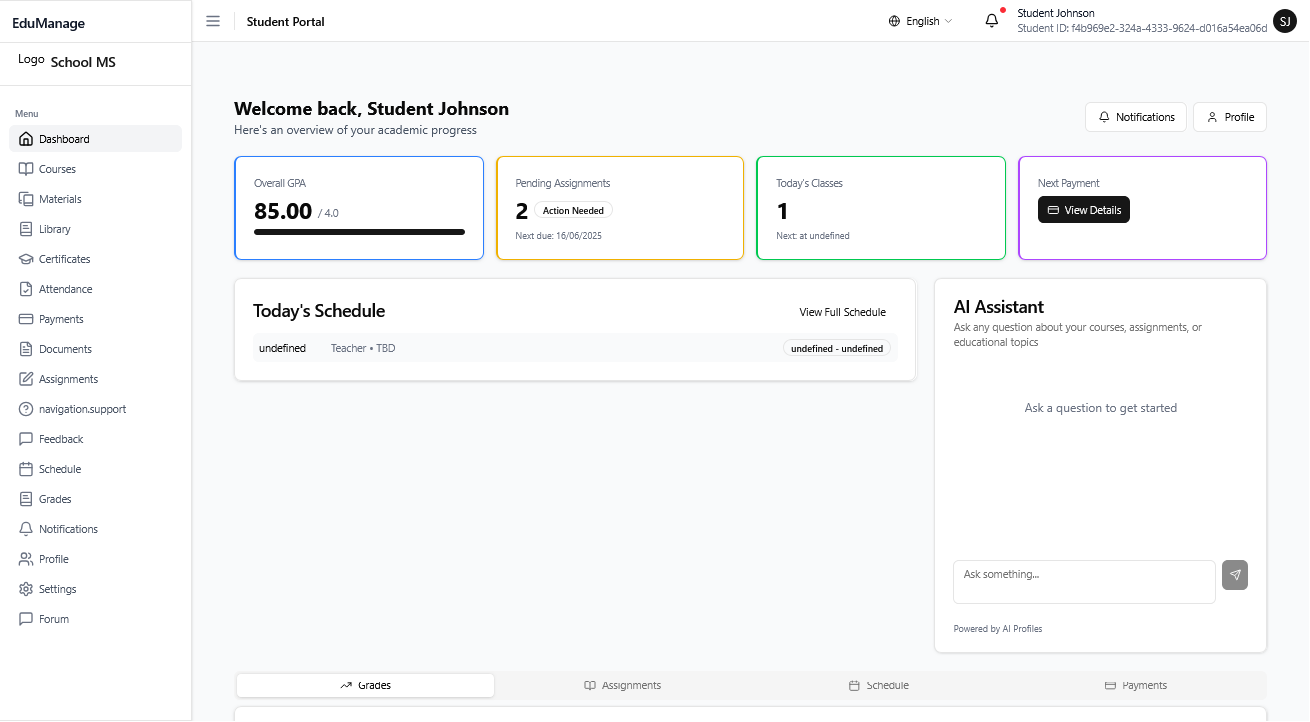
\includegraphics[width=0.85\textwidth,keepaspectratio]{pfe-pics/student/Screenshot 2025-06-09 at 22-43-56 Vite React TS.png}
  \caption{\textbf{Tableau de bord étudiant} présentant les cours, devoirs à venir et notifications.}
  \label{fig:student_dashboard}
\end{figure}

Les principales fonctionnalités pour les étudiants comprennent :

\begin{itemize}
  \item \textbf{Vue d'ensemble des cours} : Accès rapide aux cours suivis et leur contenu
  
  \item \textbf{Calendrier et échéances} : Organisation claire des devoirs et examens à venir
  
  \item \textbf{Soumission de travaux} : Interface intuitive pour déposer les devoirs
  
  \item \textbf{Consultation des résultats} : Visualisation des notes et commentaires des enseignants
\end{itemize}

\begin{figure}[H]
  \centering
  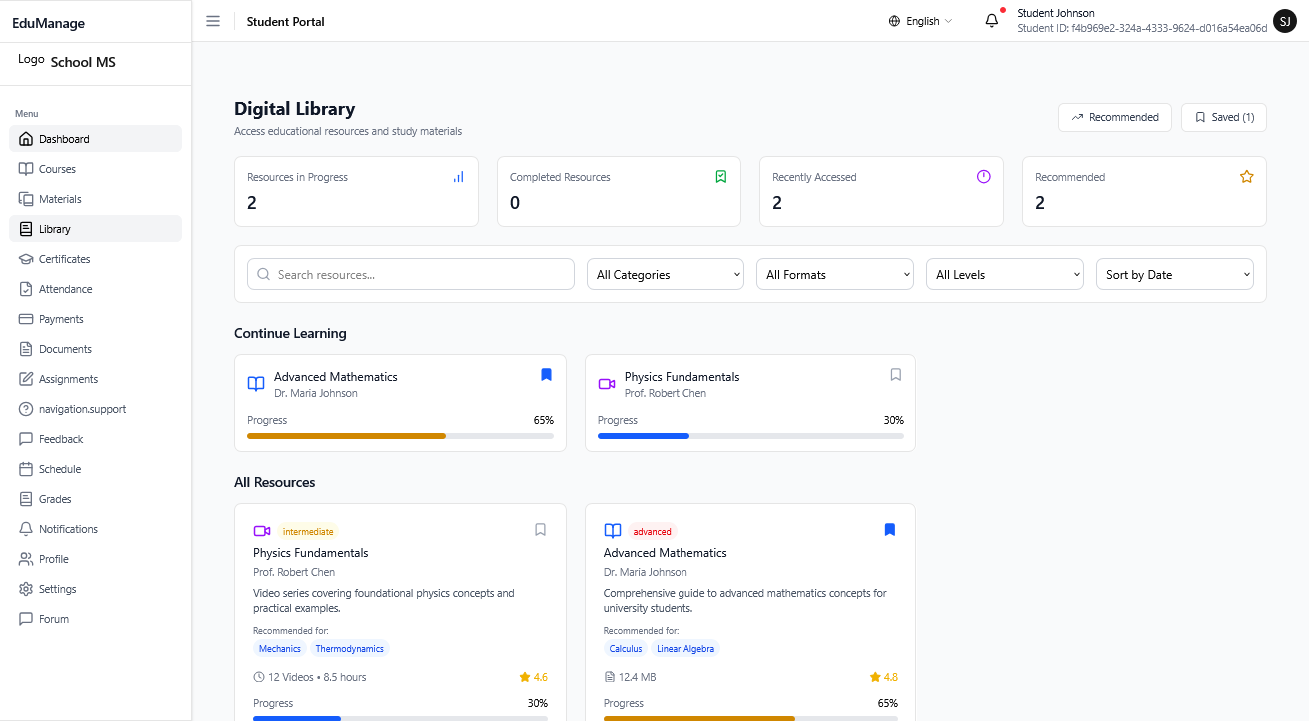
\includegraphics[width=0.85\textwidth,keepaspectratio]{pfe-pics/student/Screenshot 2025-06-09 at 22-45-09 Vite React TS.png}
  \caption{\textbf{Interface de cours} avec accès au matériel pédagogique et aux ressources.}
  \label{fig:course_view}
\end{figure}

\begin{figure}[H]
  \centering
  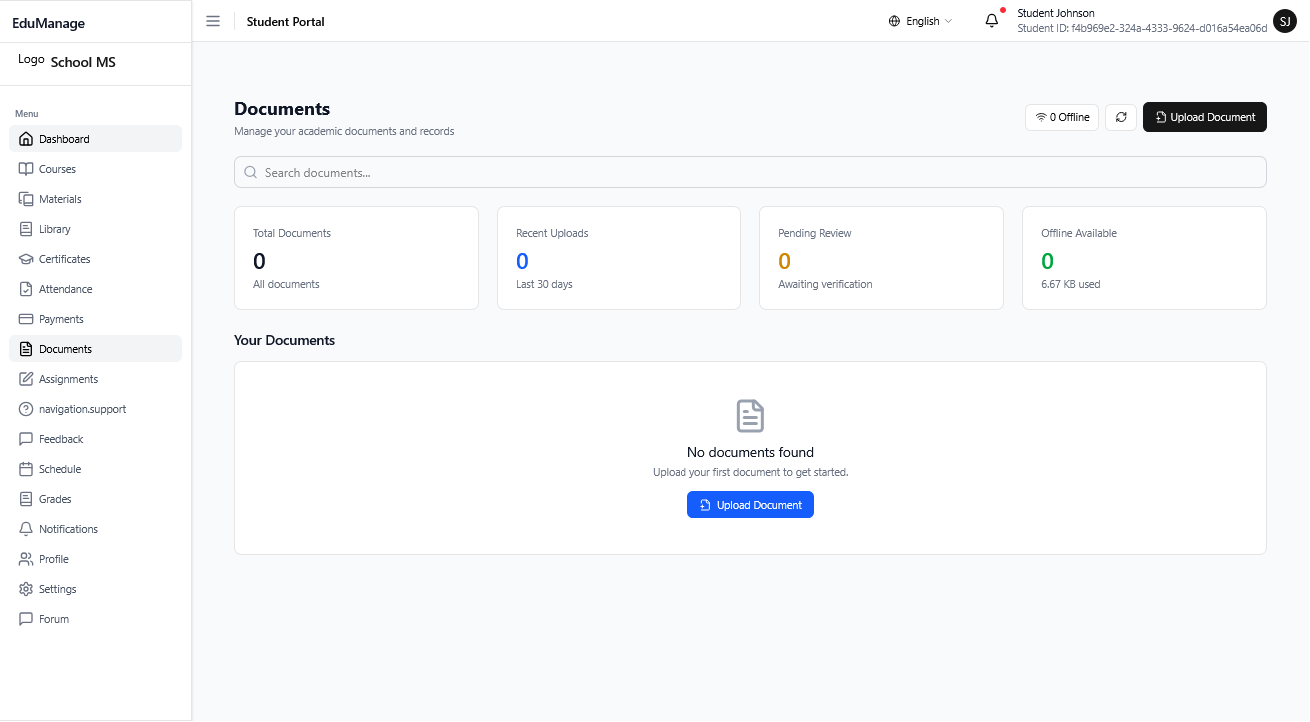
\includegraphics[width=0.85\textwidth,keepaspectratio]{pfe-pics/student/Screenshot 2025-06-09 at 22-46-22 Vite React TS.png}
  \caption{\textbf{Interface de soumission de devoir} avec options d'upload de fichiers.}
  \label{fig:assignment_submission}
\end{figure}

\subsubsection{Interface parent}

L'interface parent permet de suivre efficacement la progression académique des enfants :

\begin{figure}[H]
  \centering
  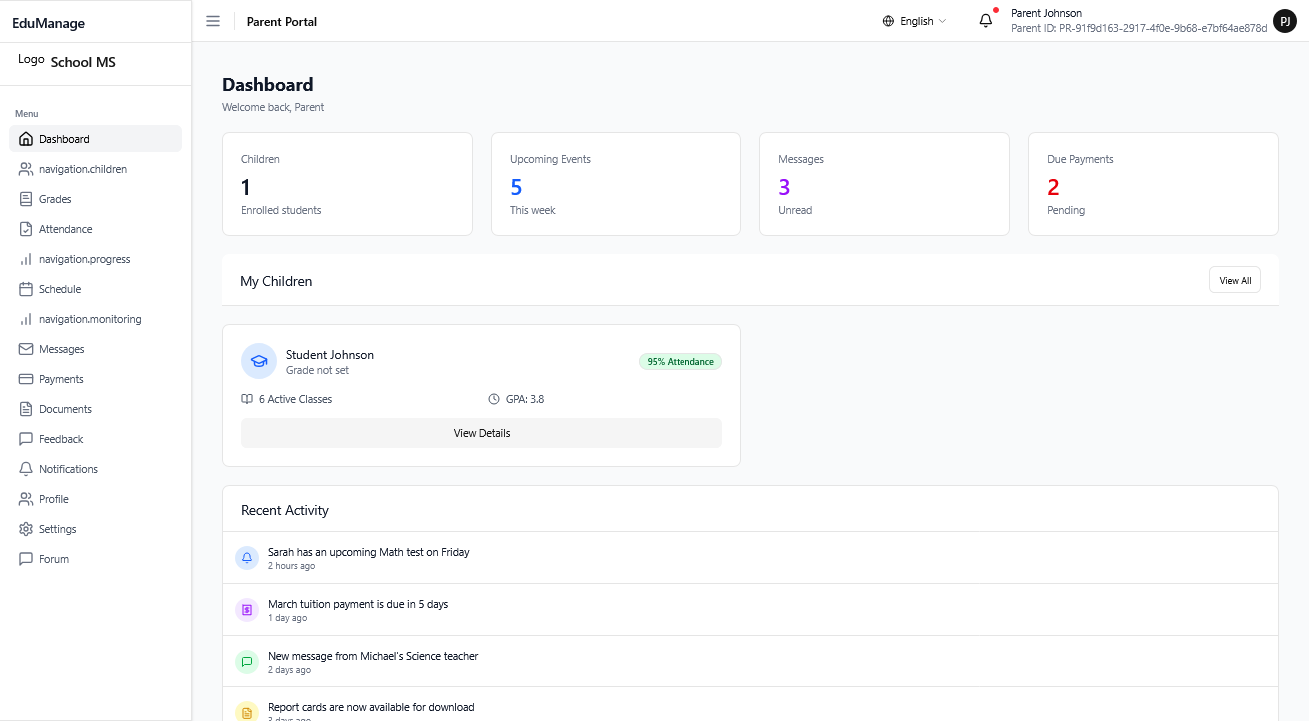
\includegraphics[width=0.85\textwidth,keepaspectratio]{pfe-pics/parent/Screenshot 2025-06-09 at 22-57-22 Vite React TS.png}
  \caption{\textbf{Tableau de bord parent} avec vue d'ensemble des enfants et leurs activités scolaires.}
  \label{fig:parent_dashboard}
\end{figure}

Les fonctionnalités développées pour les parents incluent :

\begin{itemize}
  \item \textbf{Suivi multi-enfants} : Possibilité de suivre plusieurs enfants depuis un seul compte
  
  \item \textbf{Consultation des résultats} : Accès aux notes et évaluations
  
  \item \textbf{Suivi des présences} : Visualisation de l'assiduité de l'enfant
  
  \item \textbf{Communication} : Messagerie directe avec les enseignants et l'administration
\end{itemize}

\begin{figure}[H]
  \centering
  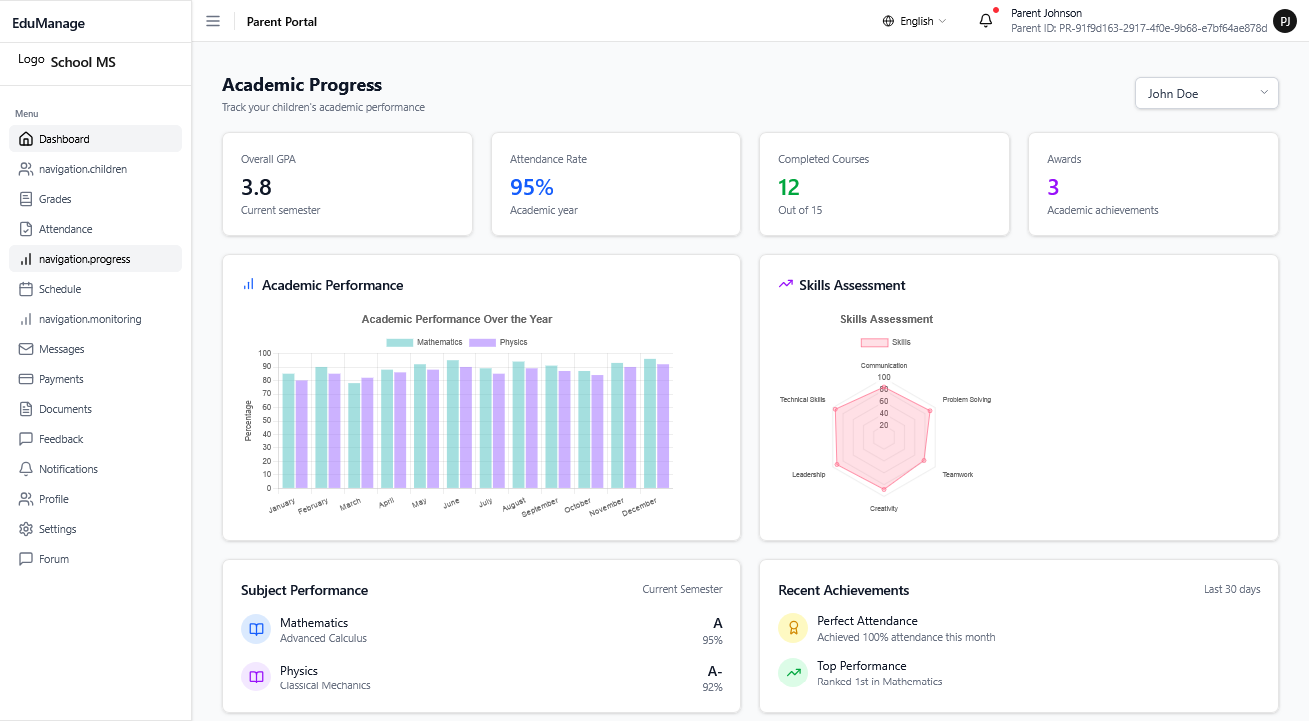
\includegraphics[width=0.85\textwidth,keepaspectratio]{pfe-pics/parent/Screenshot 2025-06-09 at 22-58-13 Vite React TS.png}
  \caption{\textbf{Interface de suivi des résultats} permettant aux parents de visualiser les performances académiques.}
  \label{fig:grades_view}
\end{figure}

\begin{figure}[H]
  \centering
  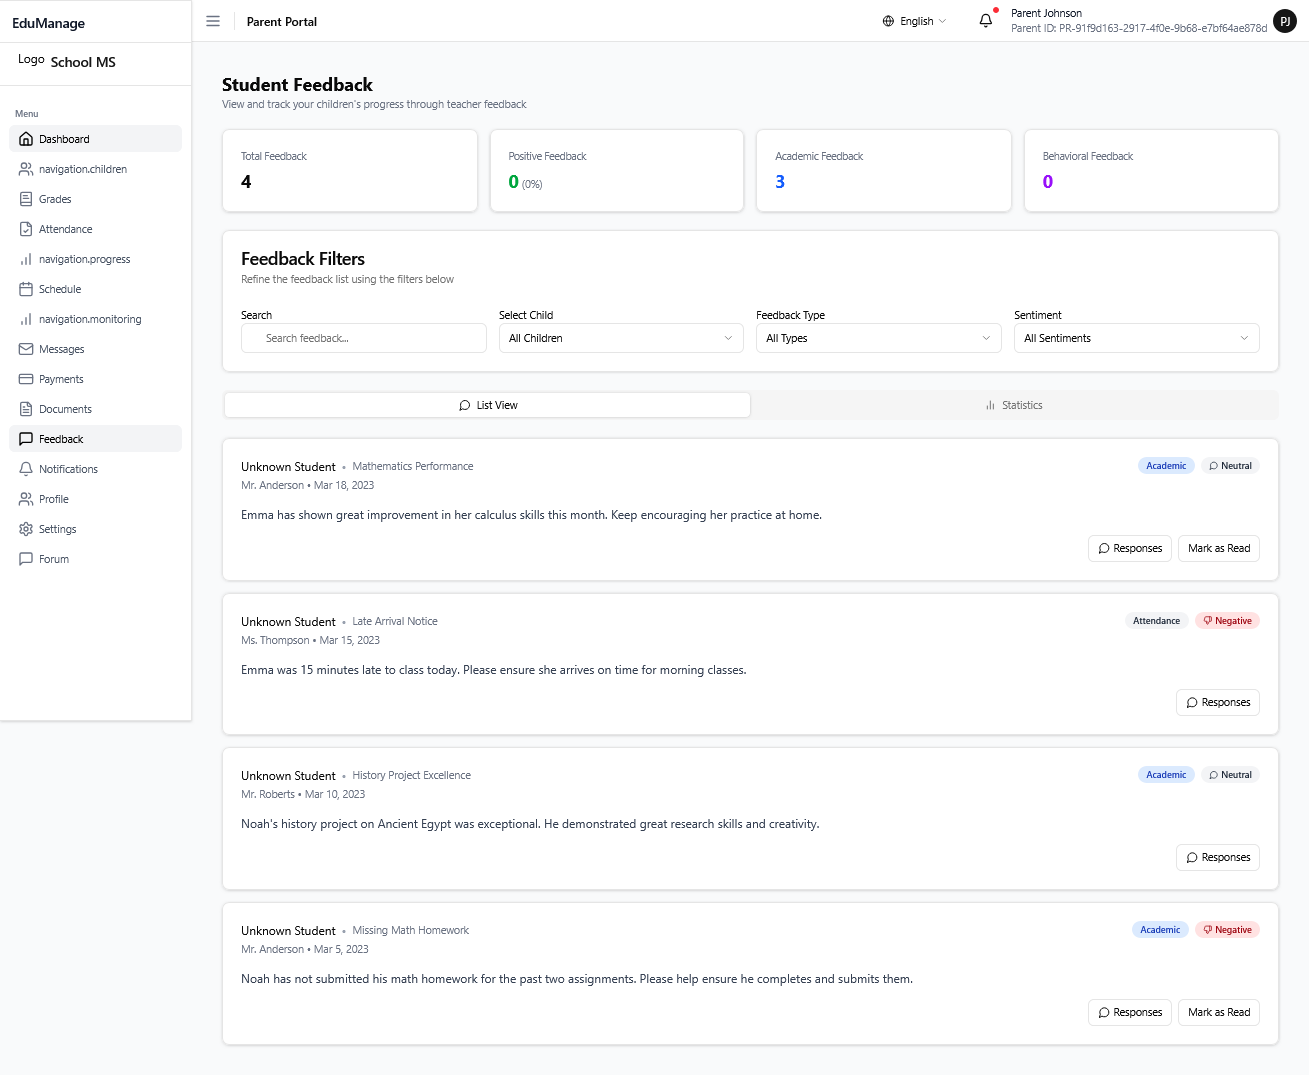
\includegraphics[width=0.85\textwidth,keepaspectratio]{pfe-pics/parent/Screenshot 2025-06-09 at 22-59-25 Vite React TS.png}
  \caption{\textbf{Interface de messagerie} pour la communication avec les enseignants.}
  \label{fig:messaging_interface}
\end{figure}

\subsubsection{Système d'authentification}

Un système d'authentification robuste a été implémenté pour sécuriser l'accès à la plateforme :

\begin{figure}[H]
  \centering
  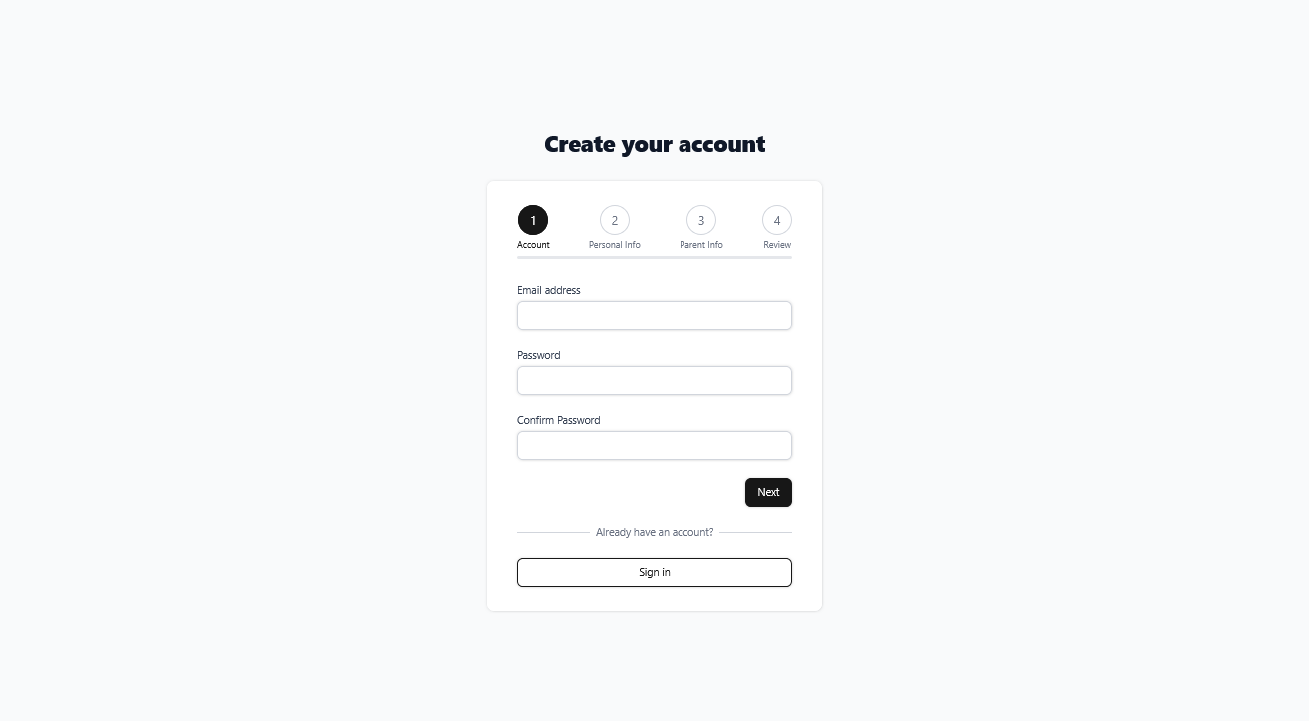
\includegraphics[width=0.6\textwidth,keepaspectratio]{pfe-pics/auth/Screenshot 2025-06-09 at 23-00-18 Vite React TS.png}
  \caption{\textbf{Page de connexion} avec sélection du type d'utilisateur.}
  \label{fig:login_page}
\end{figure}

Les fonctionnalités d'authentification comprennent :

\begin{itemize}
  \item \textbf{Connexion sécurisée} : Authentification avec email et mot de passe
  
  \item \textbf{Récupération de mot de passe} : Procédure sécurisée de réinitialisation
  
  \item \textbf{Vérification d'email} : Confirmation de l'adresse email lors de l'inscription
  
  \item \textbf{Protection des routes} : Accès contrôlé aux différentes sections selon le rôle
\end{itemize}

\begin{figure}[H]
  \centering
  
\includegraphics[width=0.6\textwidth,keepaspectratio]{pfe-pics/auth/Screenshot 2025-06-09 at 23-02-10 Vite React TS.png}
  \caption{\textbf{Interface de récupération de mot de passe} avec vérification par email.}
  \label{fig:password_reset}
\end{figure}

\begin{figure}[H]
  \centering
  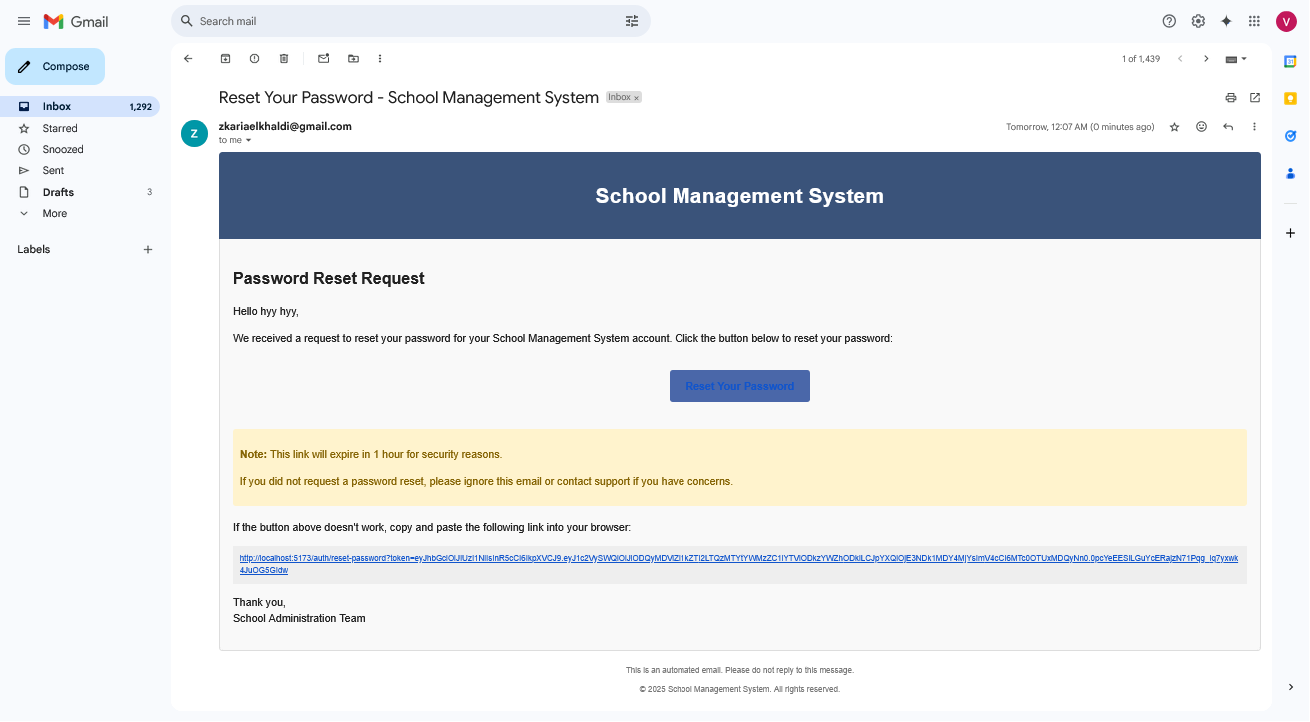
\includegraphics[width=0.85\textwidth,keepaspectratio]{pfe-pics/auth/Screenshot 2025-06-09 at 23-08-41 Reset Your Password - School Management System - vertigoevilman1@gmail.com - Gmail.png}
  \caption{\textbf{Email de réinitialisation de mot de passe} envoyé aux utilisateurs.}
  \label{fig:password_reset_email}
\end{figure}

\subsection{Développement des applications mobiles}

\subsubsection{Architecture de l'application mobile}

L'application mobile a été développée avec React Native et Expo pour offrir une expérience utilisateur native sur iOS et Android tout en partageant une base de code commune. L'architecture adoptée suit le modèle de composants React avec une gestion d'état centralisée.

\begin{itemize}
  \item \textbf{Structure du projet} : Organisation en modules fonctionnels avec séparation des préoccupations
  
  \item \textbf{Navigation} : Utilisation de React Navigation pour une expérience de navigation fluide
  
  \item \textbf{Gestion d'état} : Combinaison de Context API et de React Query pour la gestion des données
  
  \item \textbf{Composants réutilisables} : Bibliothèque de composants partagés entre les différentes vues
  
  \item \textbf{Adaptation responsive} : Interfaces s'adaptant aux différentes tailles d'écran
\end{itemize}

\subsubsection{Interfaces mobiles pour les étudiants}

L'application mobile offre aux étudiants un accès optimisé à leurs cours et activités :

\begin{figure}[H]
  \centering
  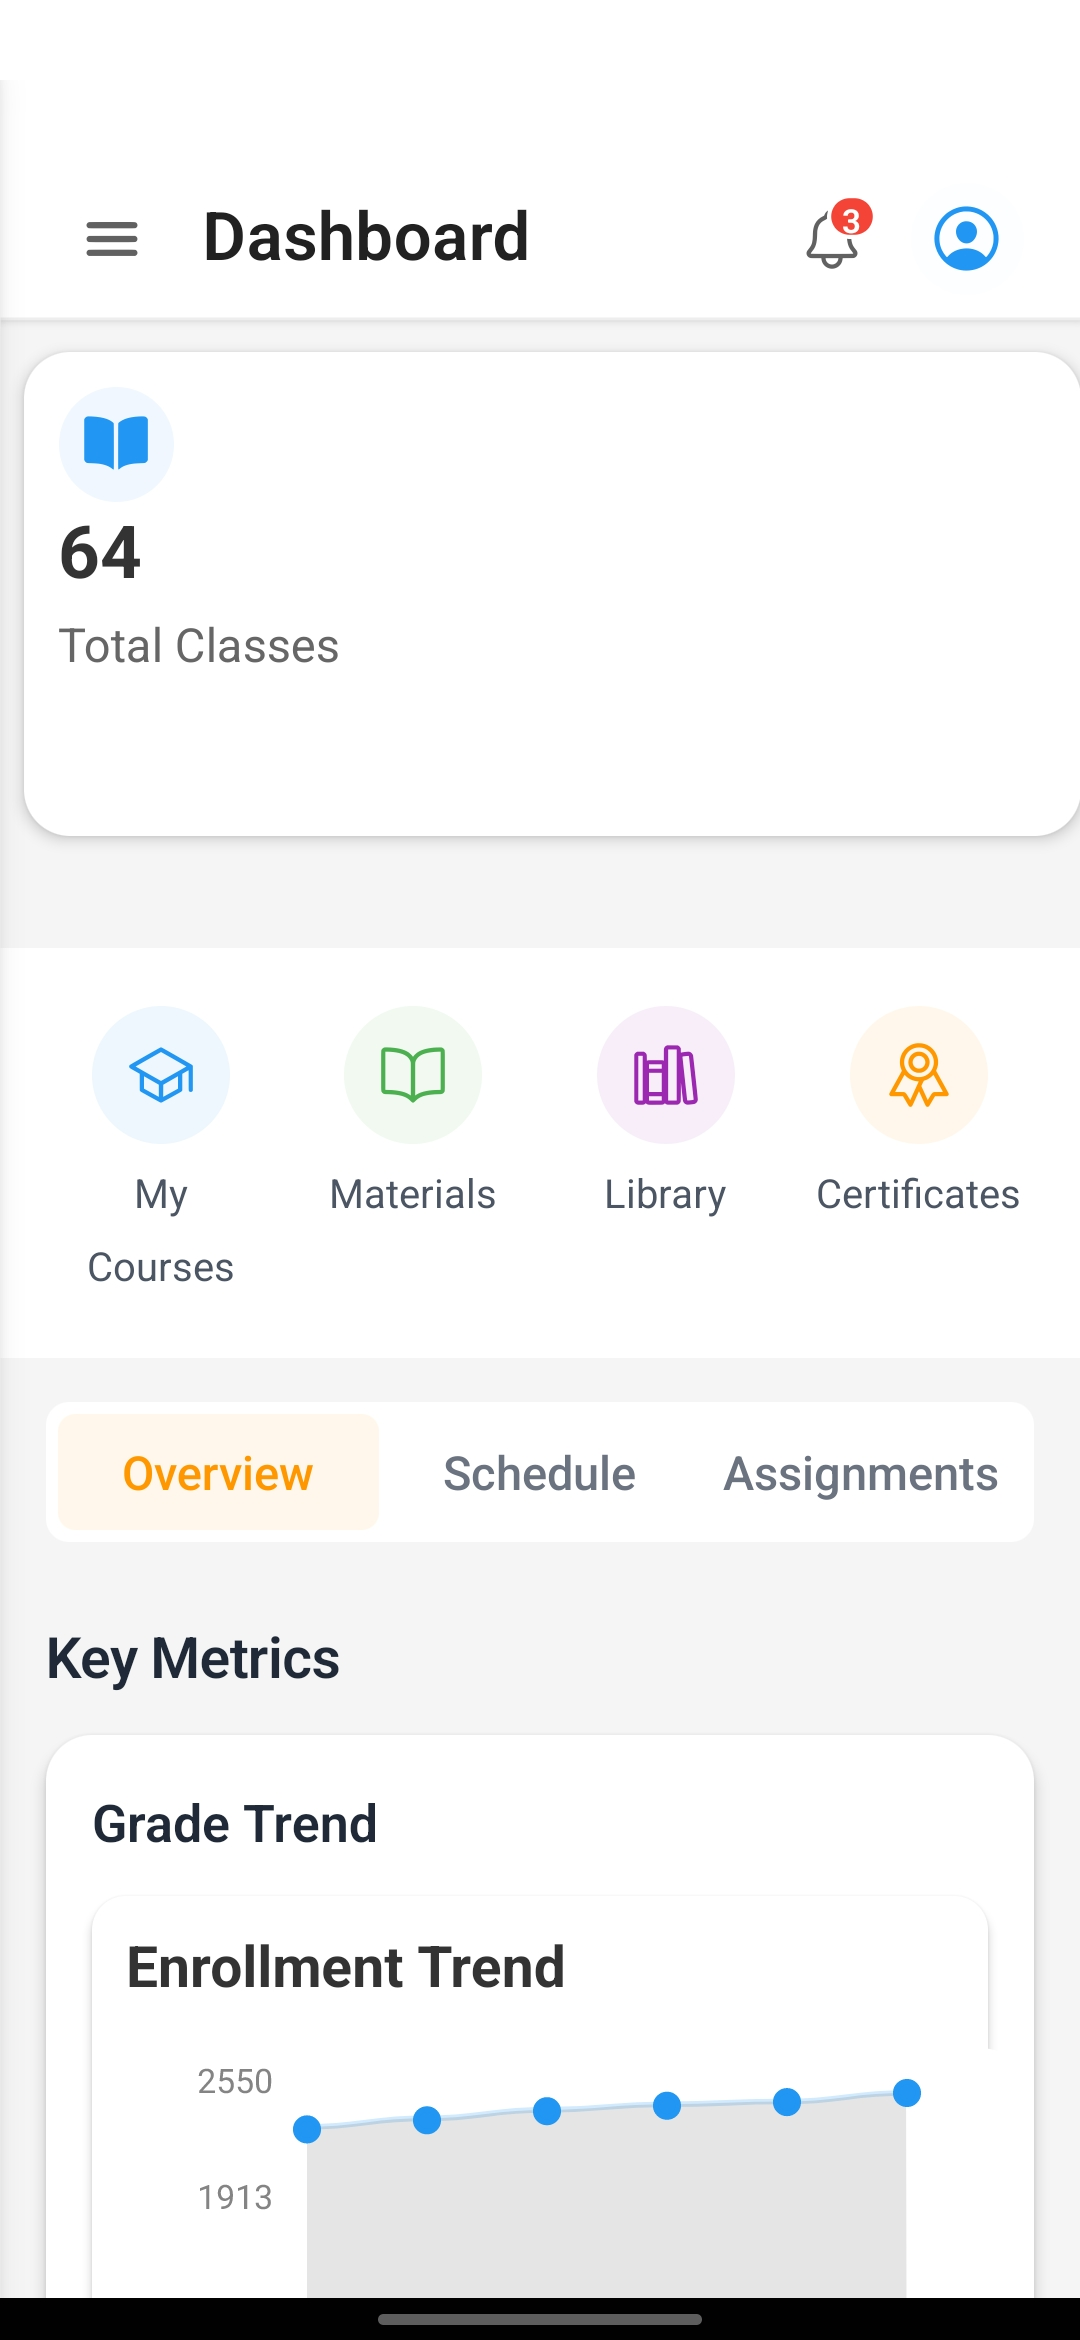
\includegraphics[width=0.4\textwidth,keepaspectratio]{pfe-pics/Mobile /Students/Screenshot_20250610_130022_Expo Go.jpg}
  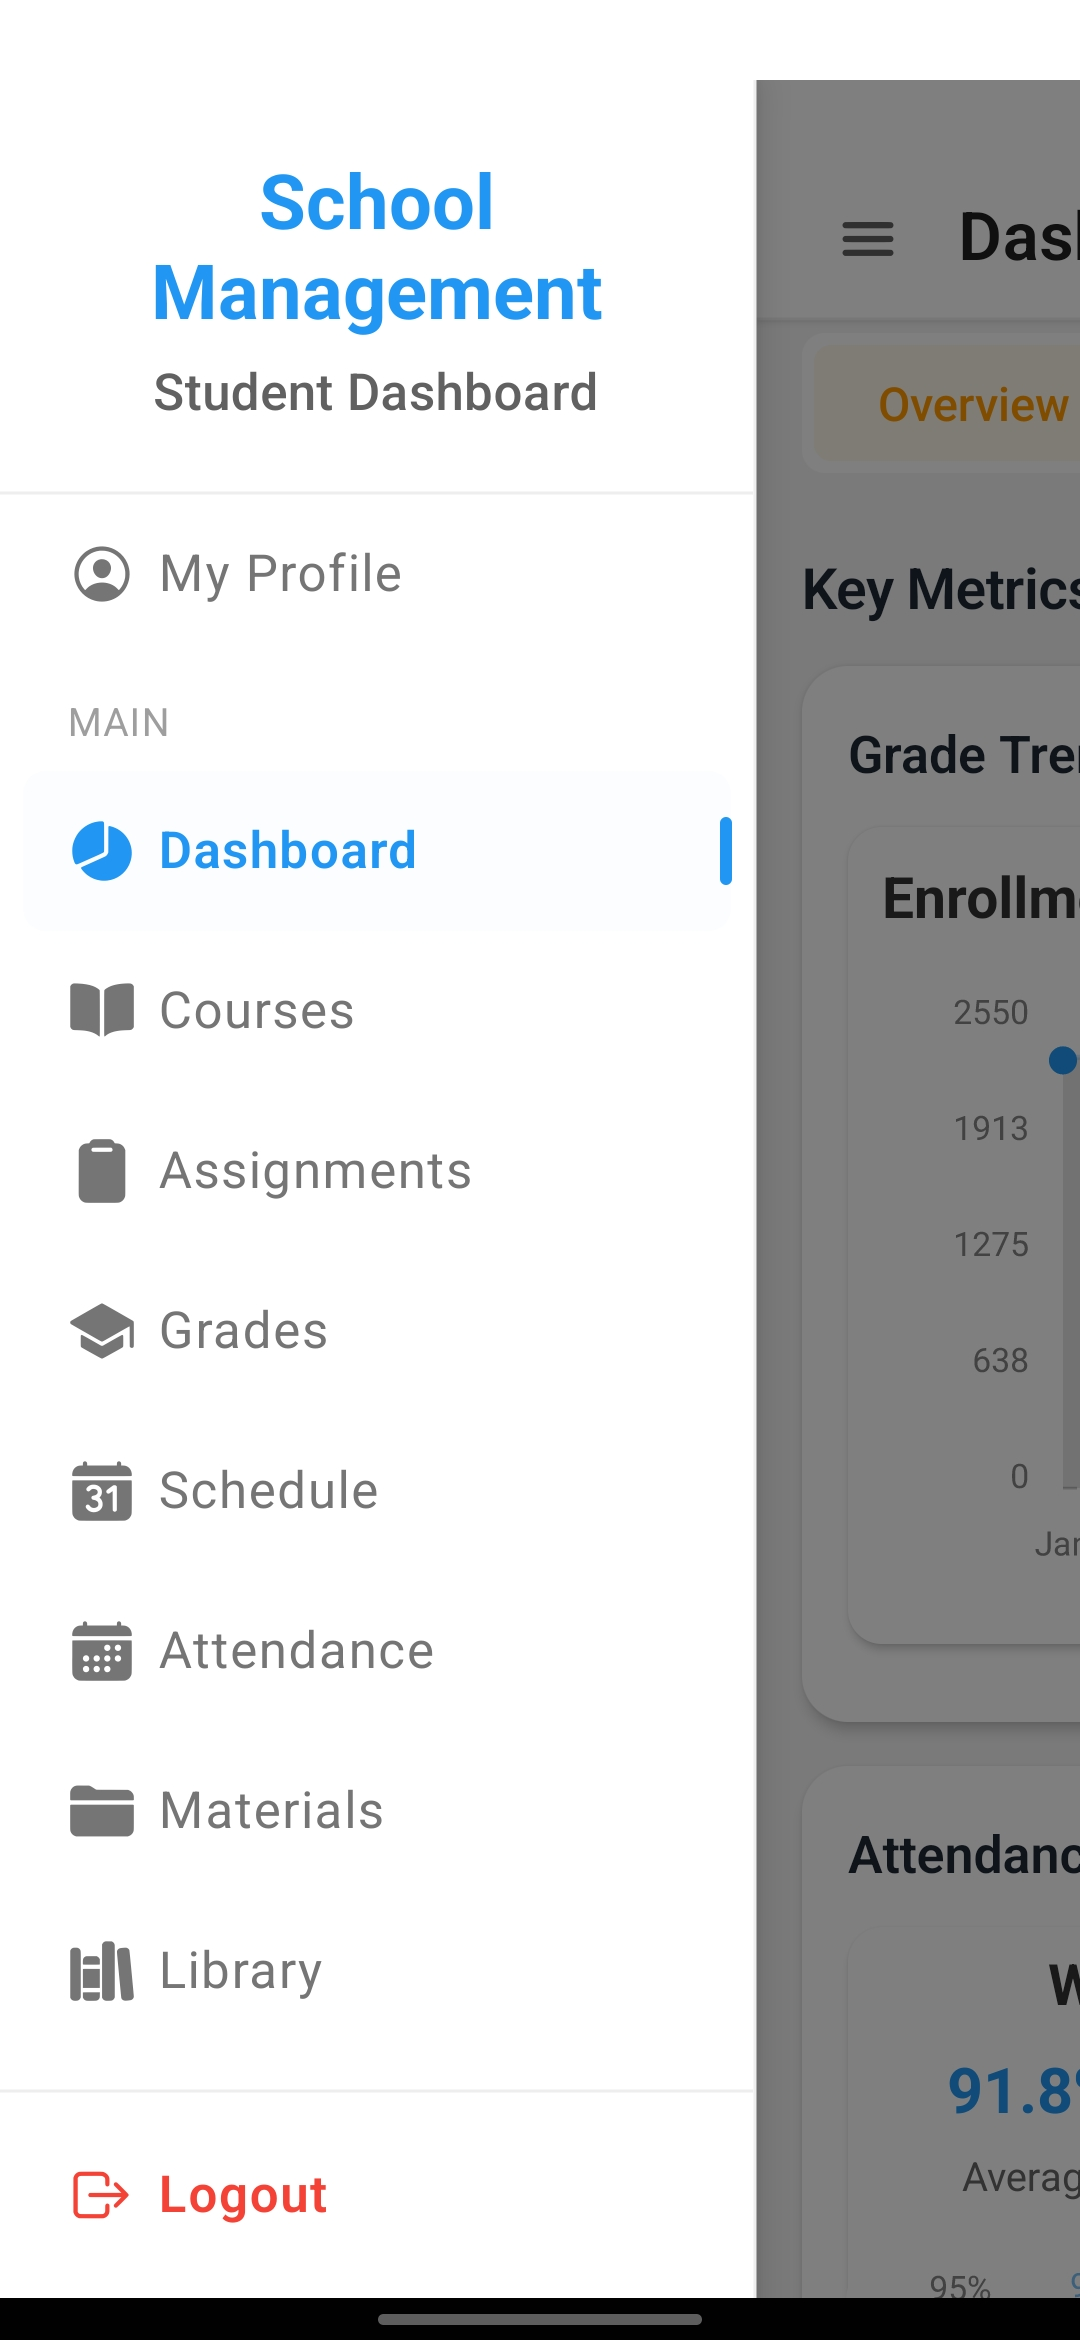
\includegraphics[width=0.4\textwidth,keepaspectratio]{pfe-pics/Mobile /Students/Screenshot_20250610_130124_Expo Go.jpg}
  \caption{\textbf{Écrans d'accueil et de cours} de l'application mobile pour les étudiants.}
  \label{fig:mobile_student_home}
\end{figure}

\begin{figure}[H]
  \centering
  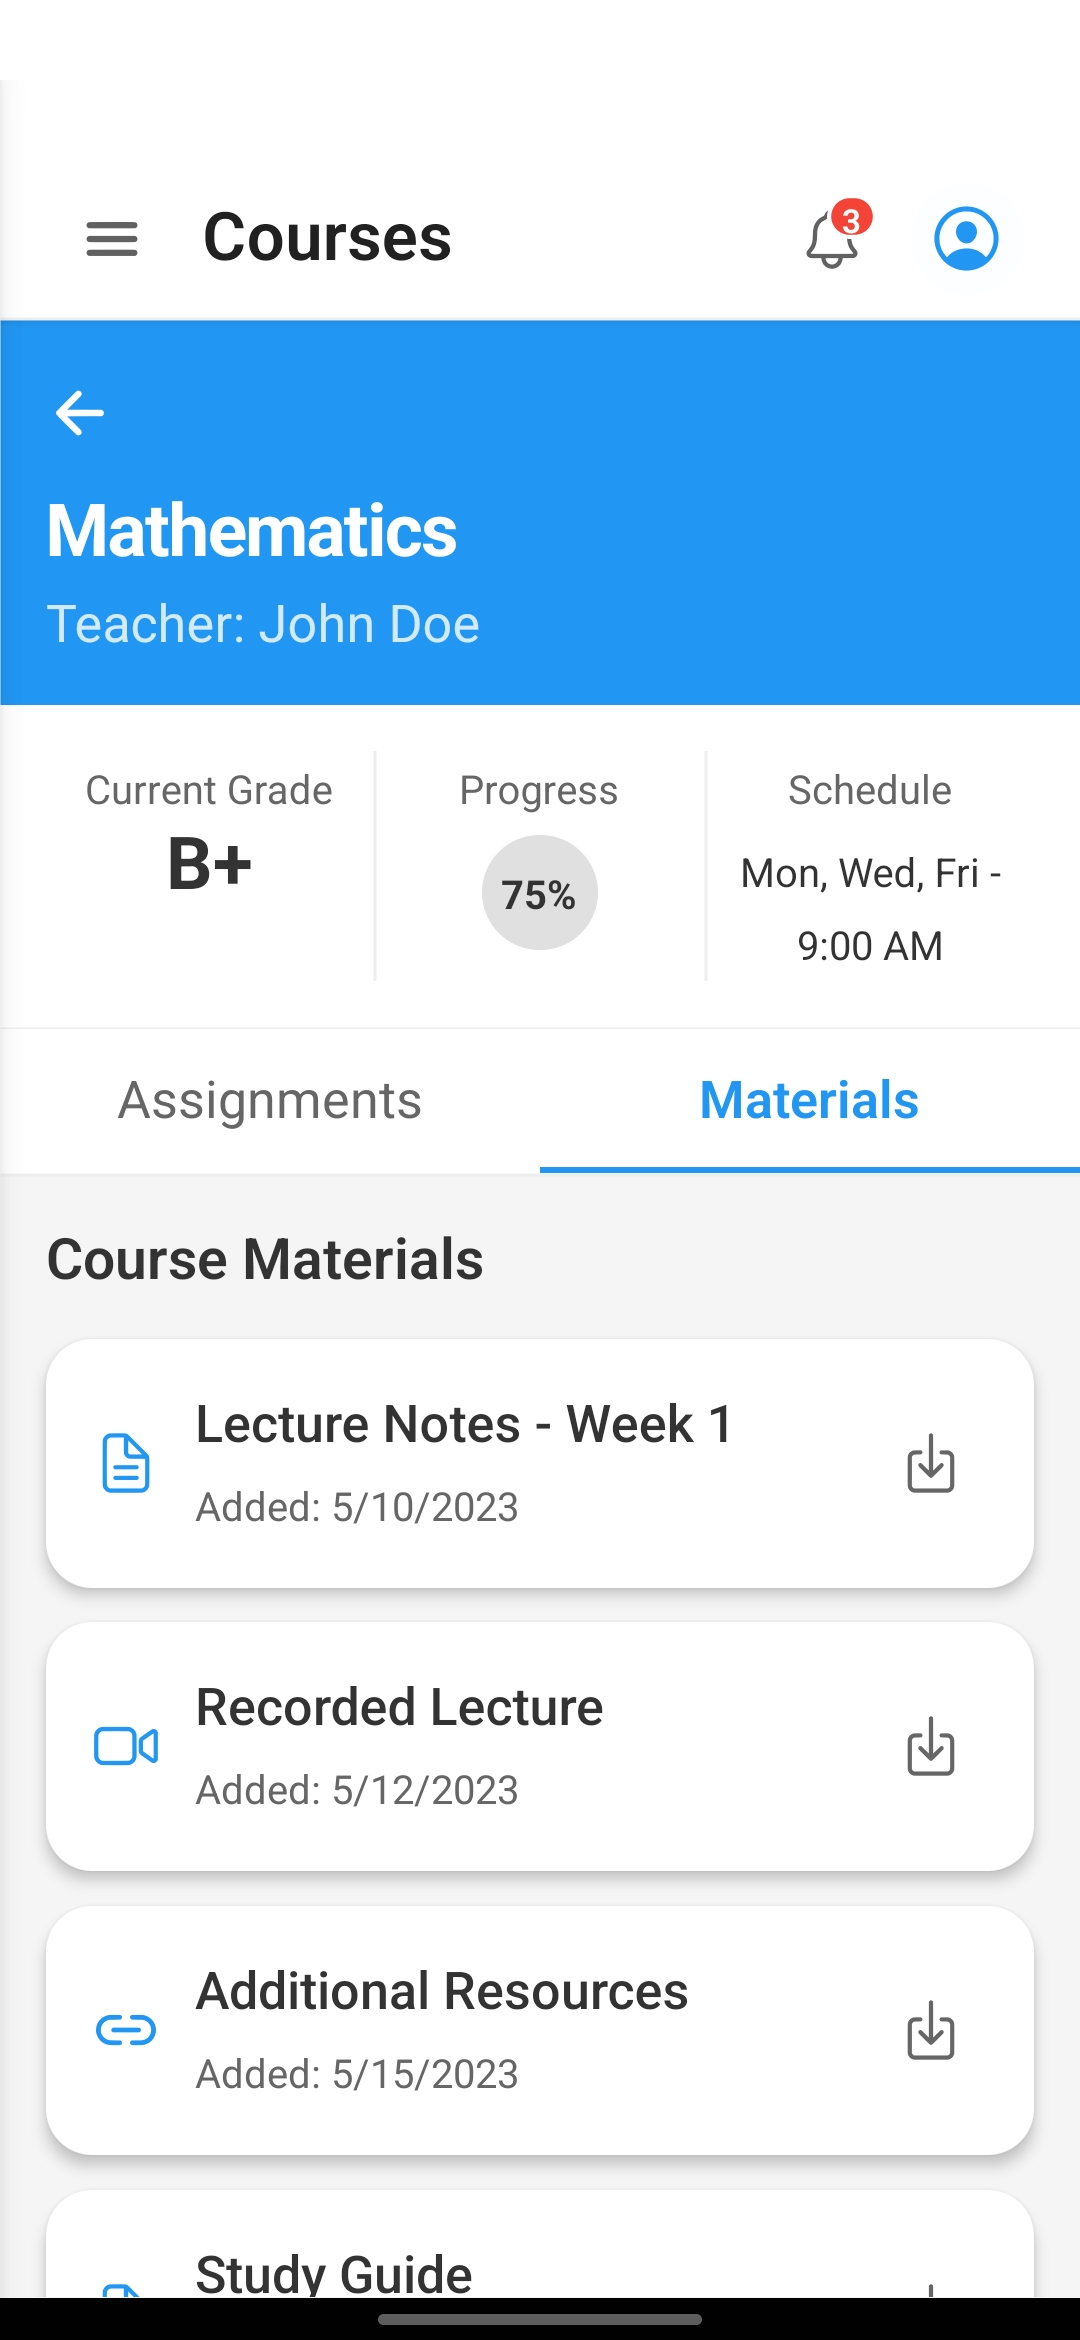
\includegraphics[width=0.4\textwidth,keepaspectratio]{pfe-pics/Mobile /Students/Screenshot_20250610_130150_Expo Go.jpg}
  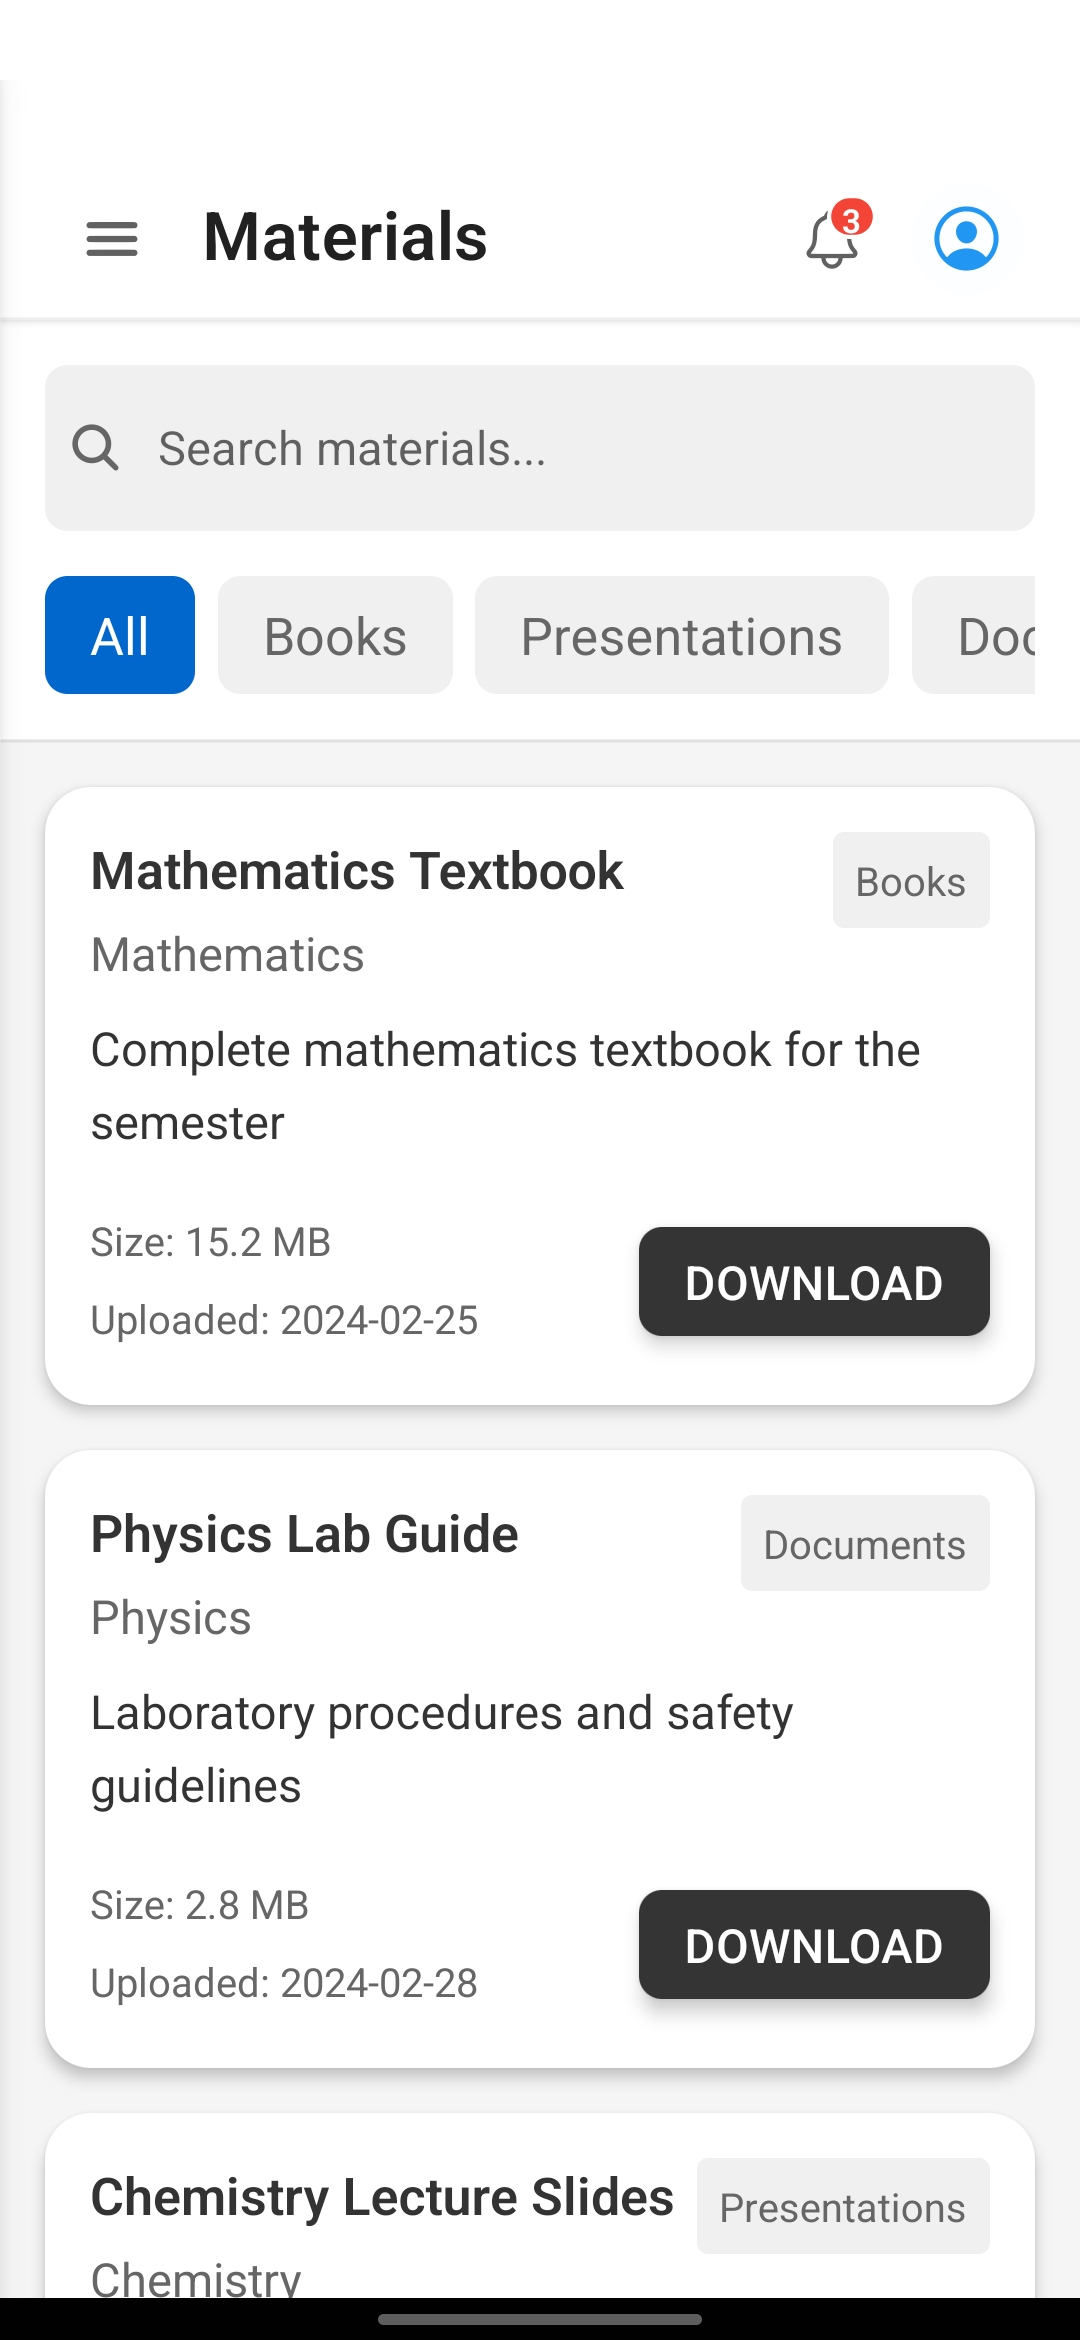
\includegraphics[width=0.4\textwidth,keepaspectratio]{pfe-pics/Mobile /Students/Screenshot_20250610_130310_Expo Go.jpg}
  \caption{\textbf{Interfaces de consultation des devoirs et résultats} sur mobile.}
  \label{fig:mobile_student_assignments}
\end{figure}

\subsubsection{Interfaces mobiles pour les enseignants}

Les enseignants bénéficient d'une application mobile adaptée à leurs besoins spécifiques :

\begin{figure}[H]
  \centering
  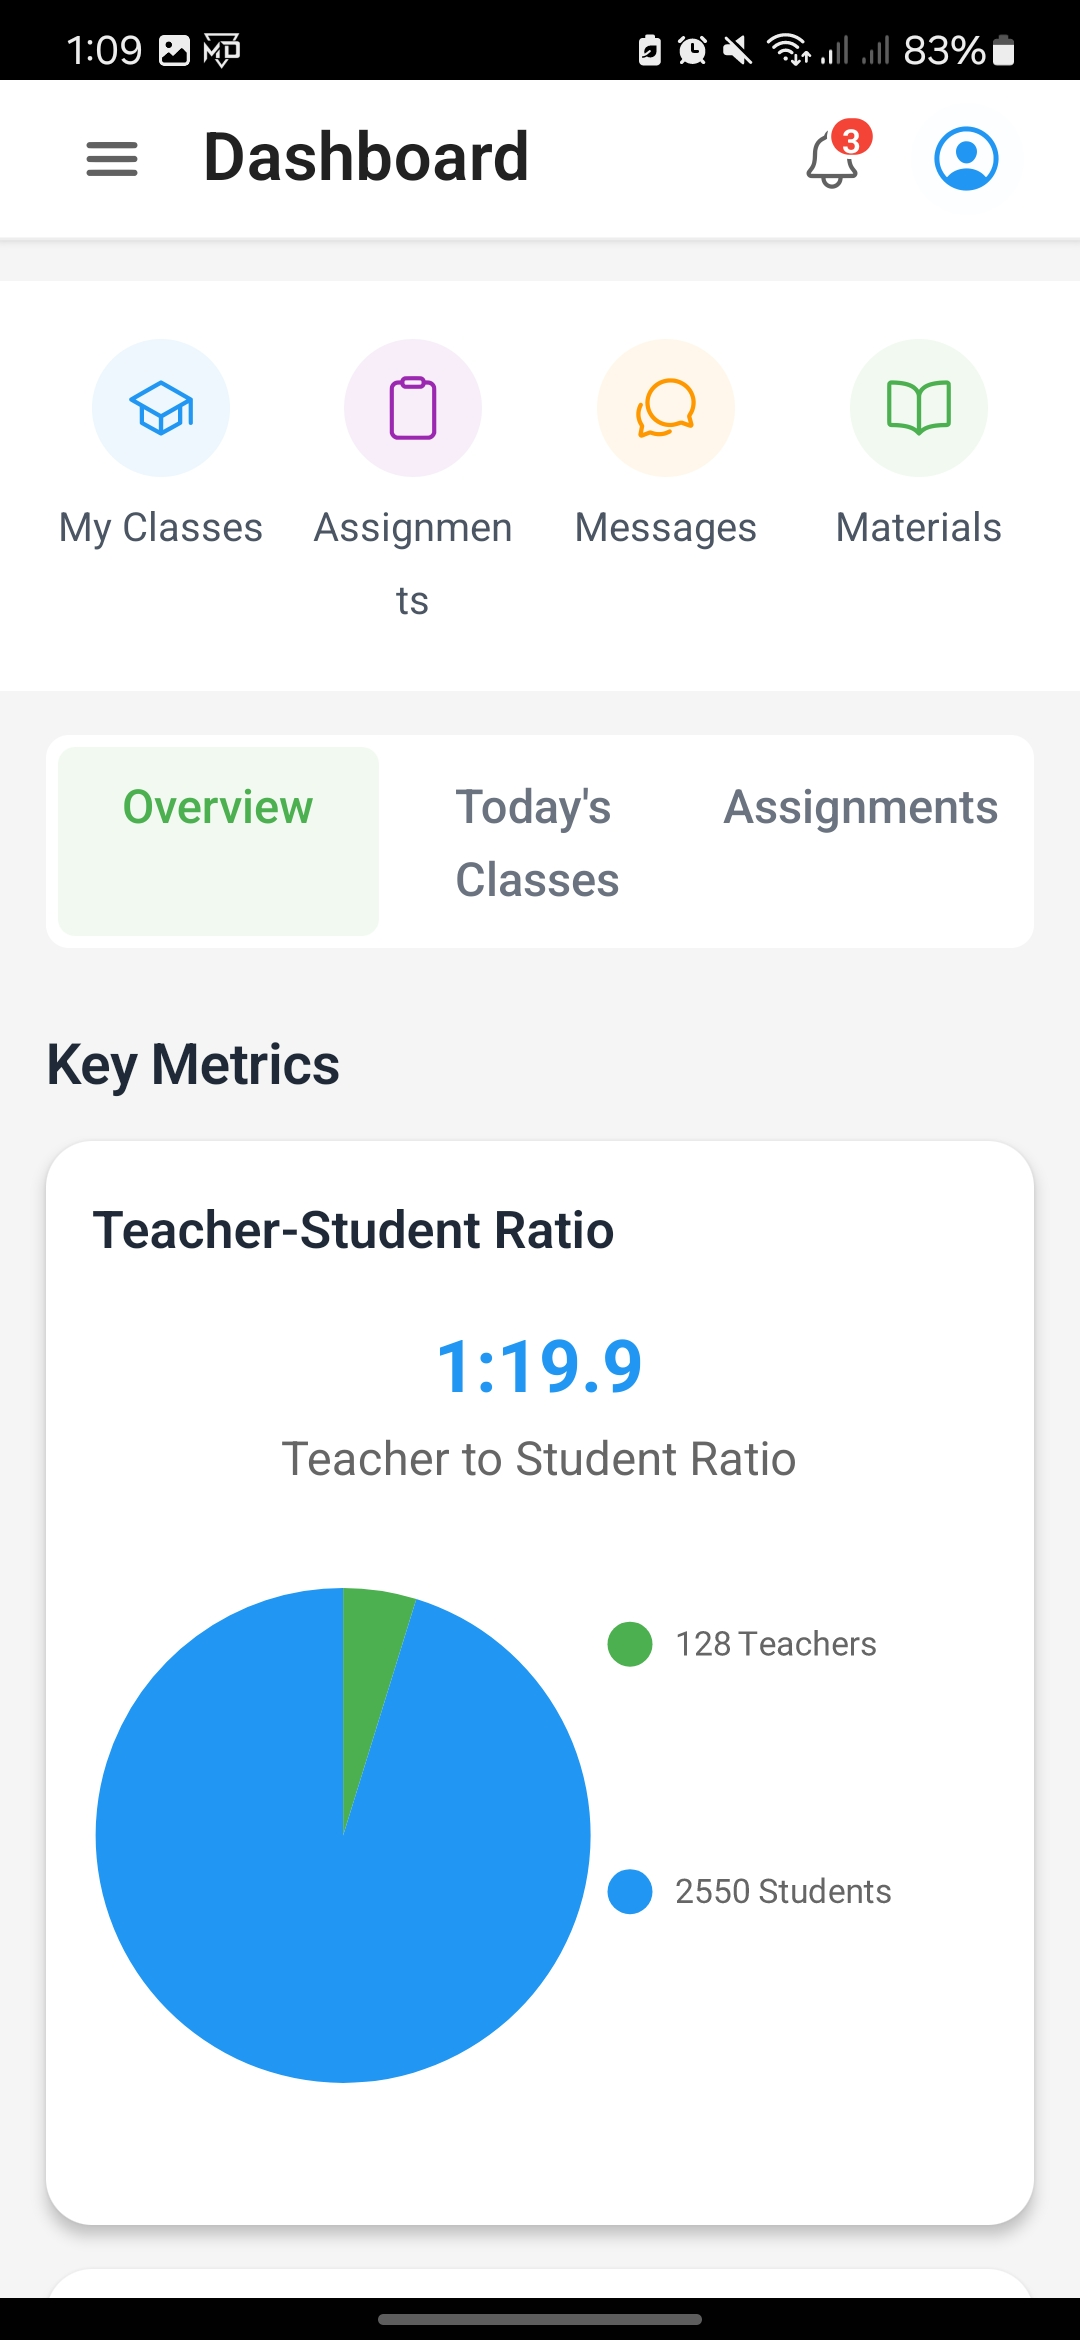
\includegraphics[width=0.4\textwidth,keepaspectratio]{pfe-pics/Mobile /Teacher/Screenshot_20250610_130952_Expo Go.jpg}
  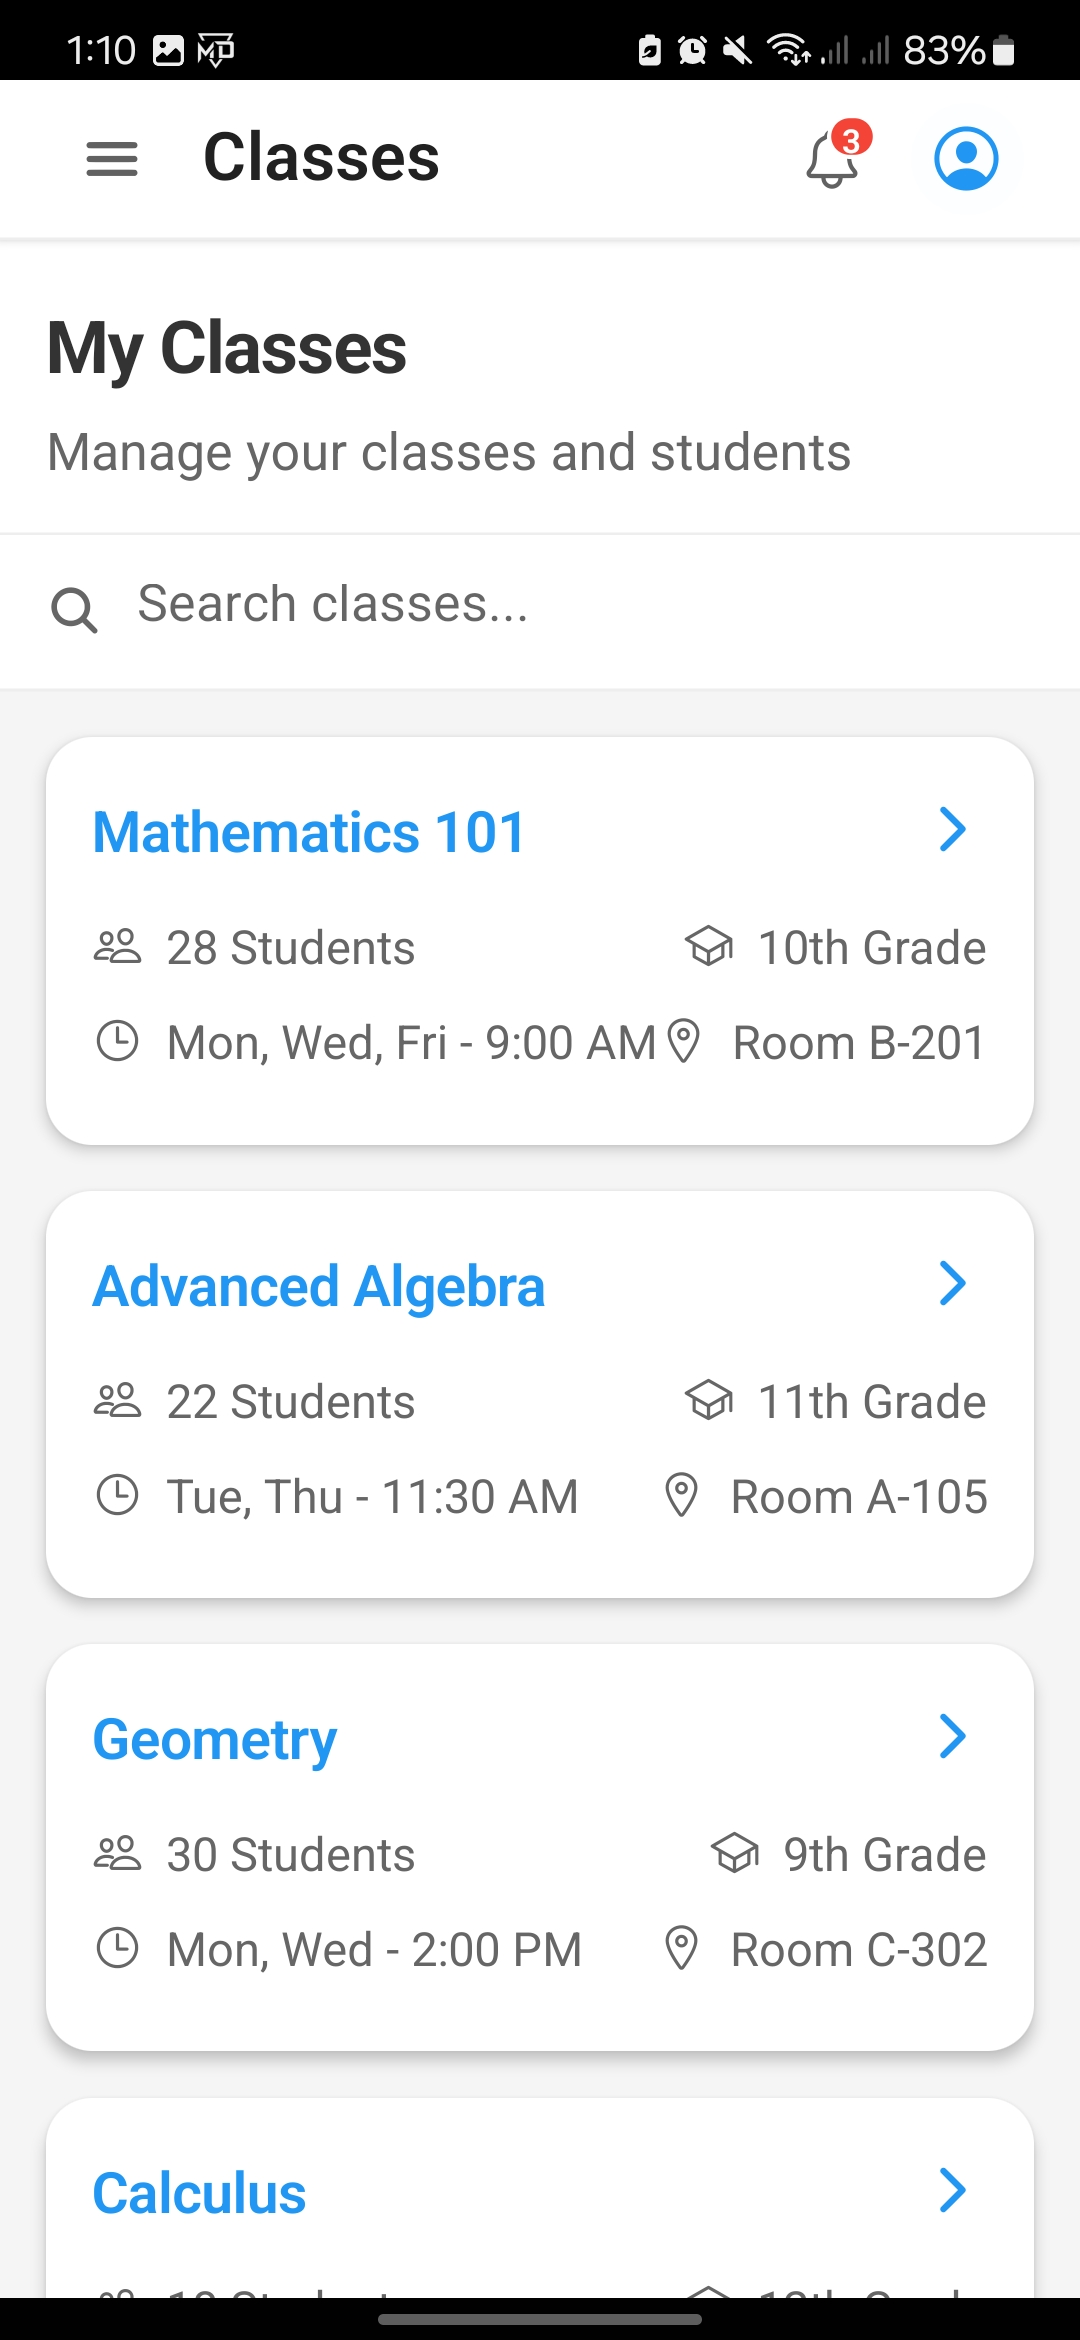
\includegraphics[width=0.4\textwidth,keepaspectratio]{pfe-pics/Mobile /Teacher/Screenshot_20250610_131009_Expo Go.jpg}
  \caption{\textbf{Tableau de bord et liste des cours} sur l'application mobile enseignant.}
  \label{fig:mobile_teacher_dashboard}
\end{figure}

\begin{figure}[H]
  \centering
  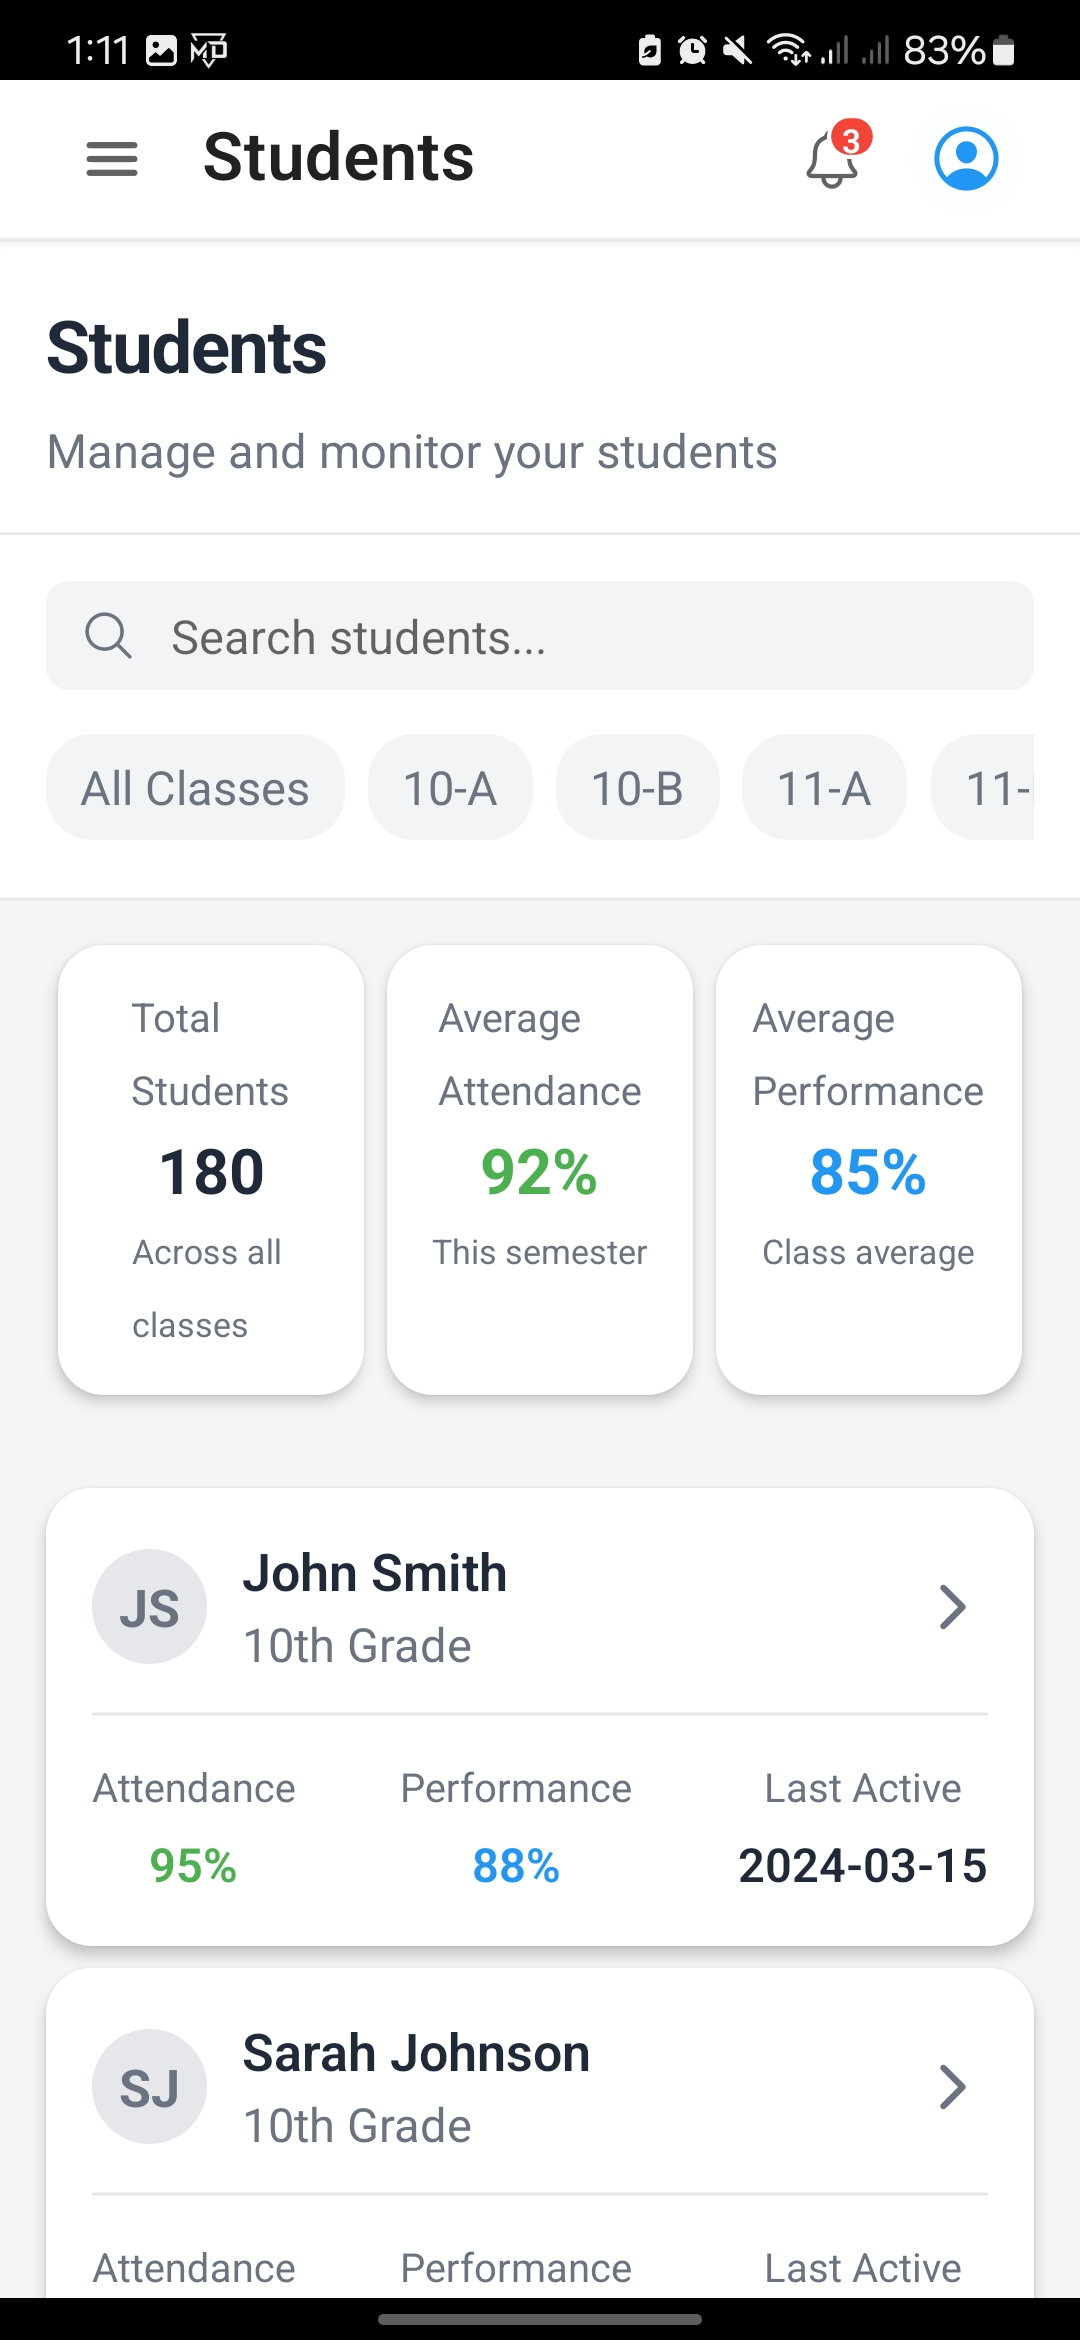
\includegraphics[width=0.4\textwidth,keepaspectratio]{pfe-pics/Mobile /Teacher/Screenshot_20250610_131112_Expo Go.jpg}
  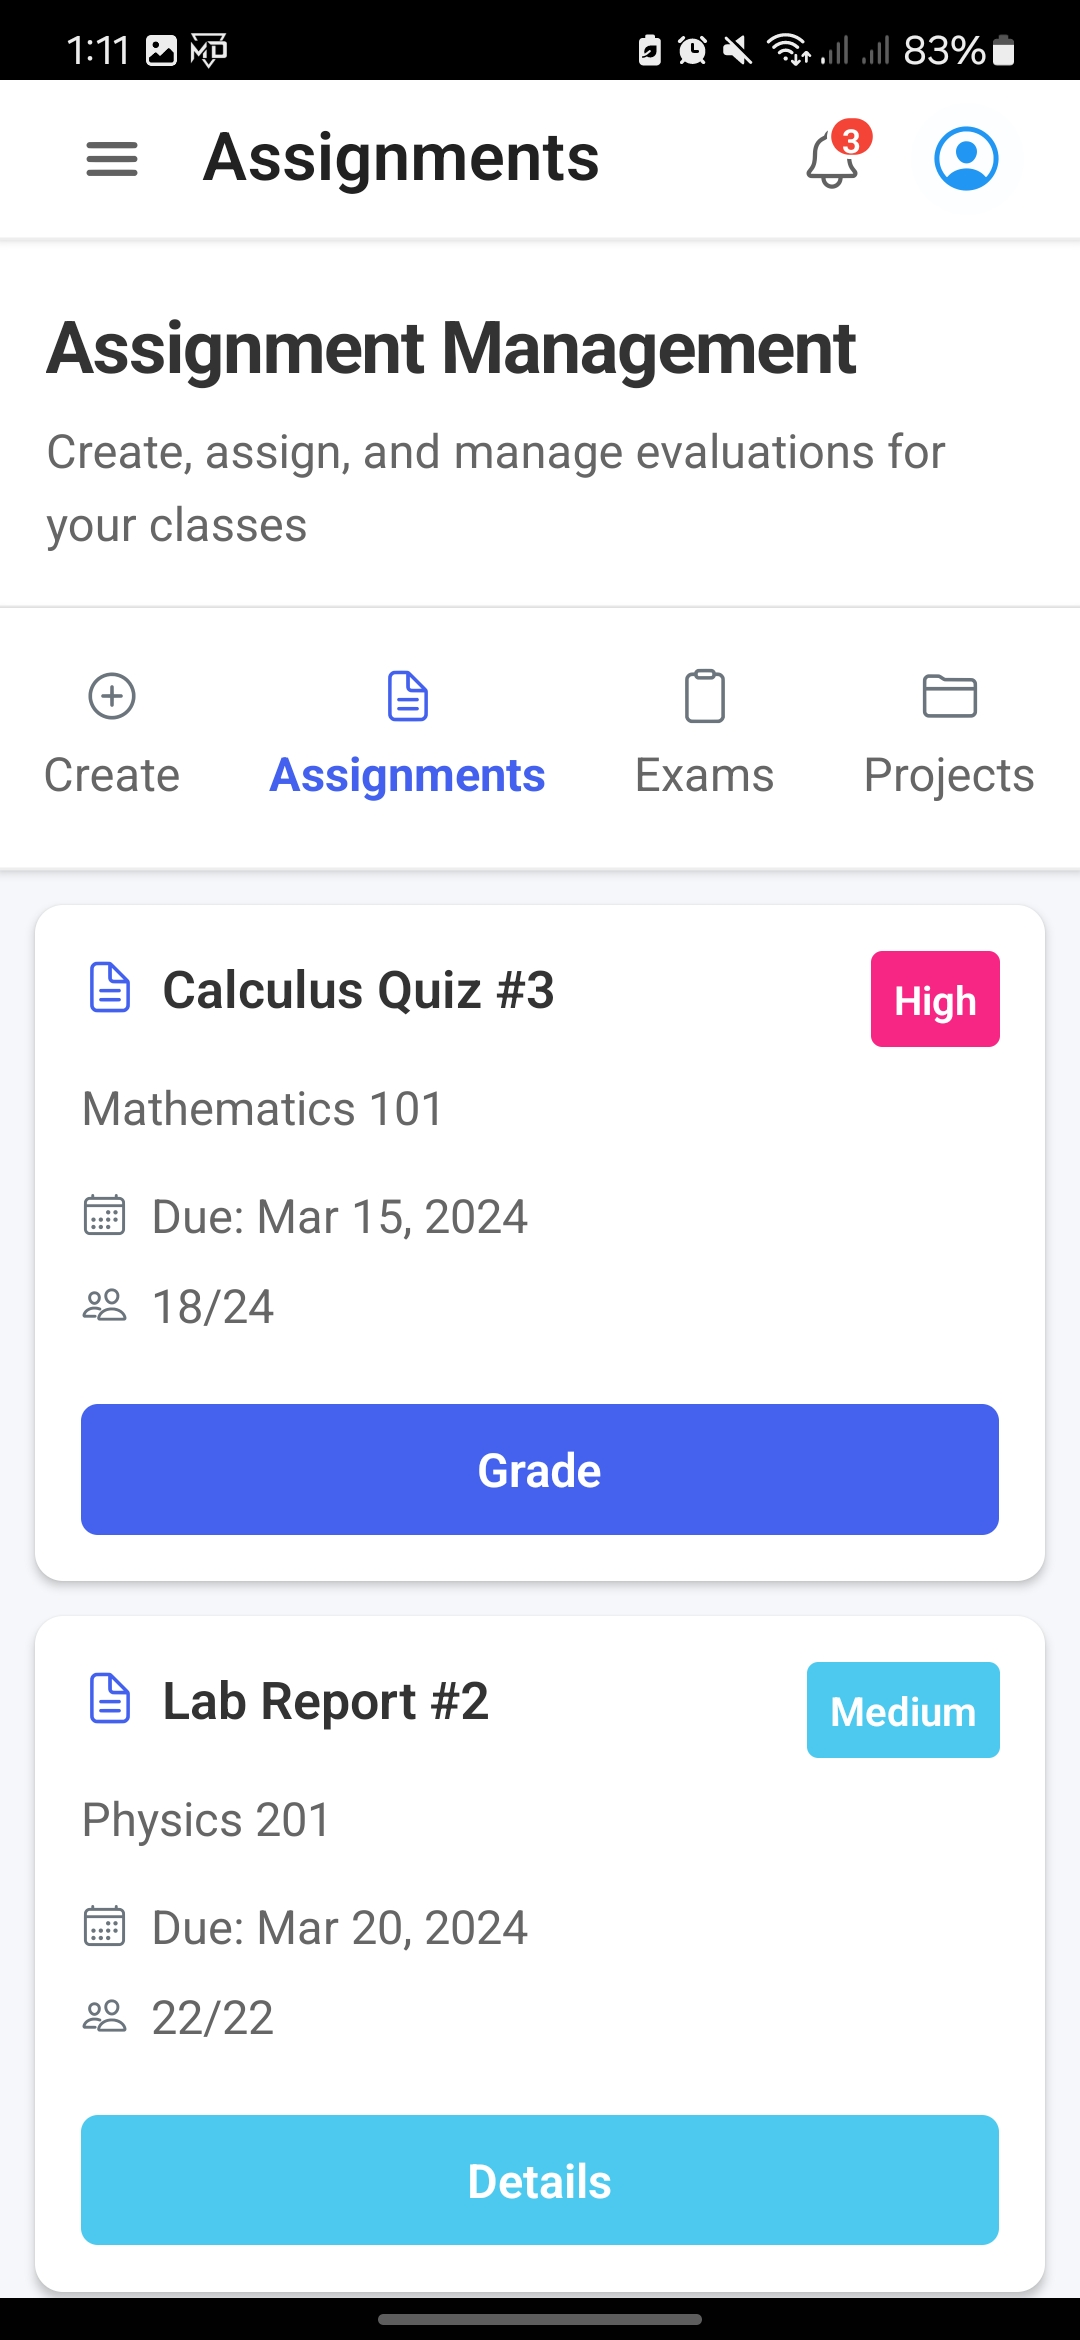
\includegraphics[width=0.4\textwidth,keepaspectratio]{pfe-pics/Mobile /Teacher/Screenshot_20250610_131132_Expo Go.jpg}
  \caption{\textbf{Interfaces de prise de présence et de notation} optimisées pour mobile.}
  \label{fig:mobile_teacher_attendance}
\end{figure}

\subsubsection{Interfaces mobiles pour les parents}

L'application mobile pour les parents facilite le suivi des activités scolaires de leurs enfants :

\begin{figure}[H]
  \centering
  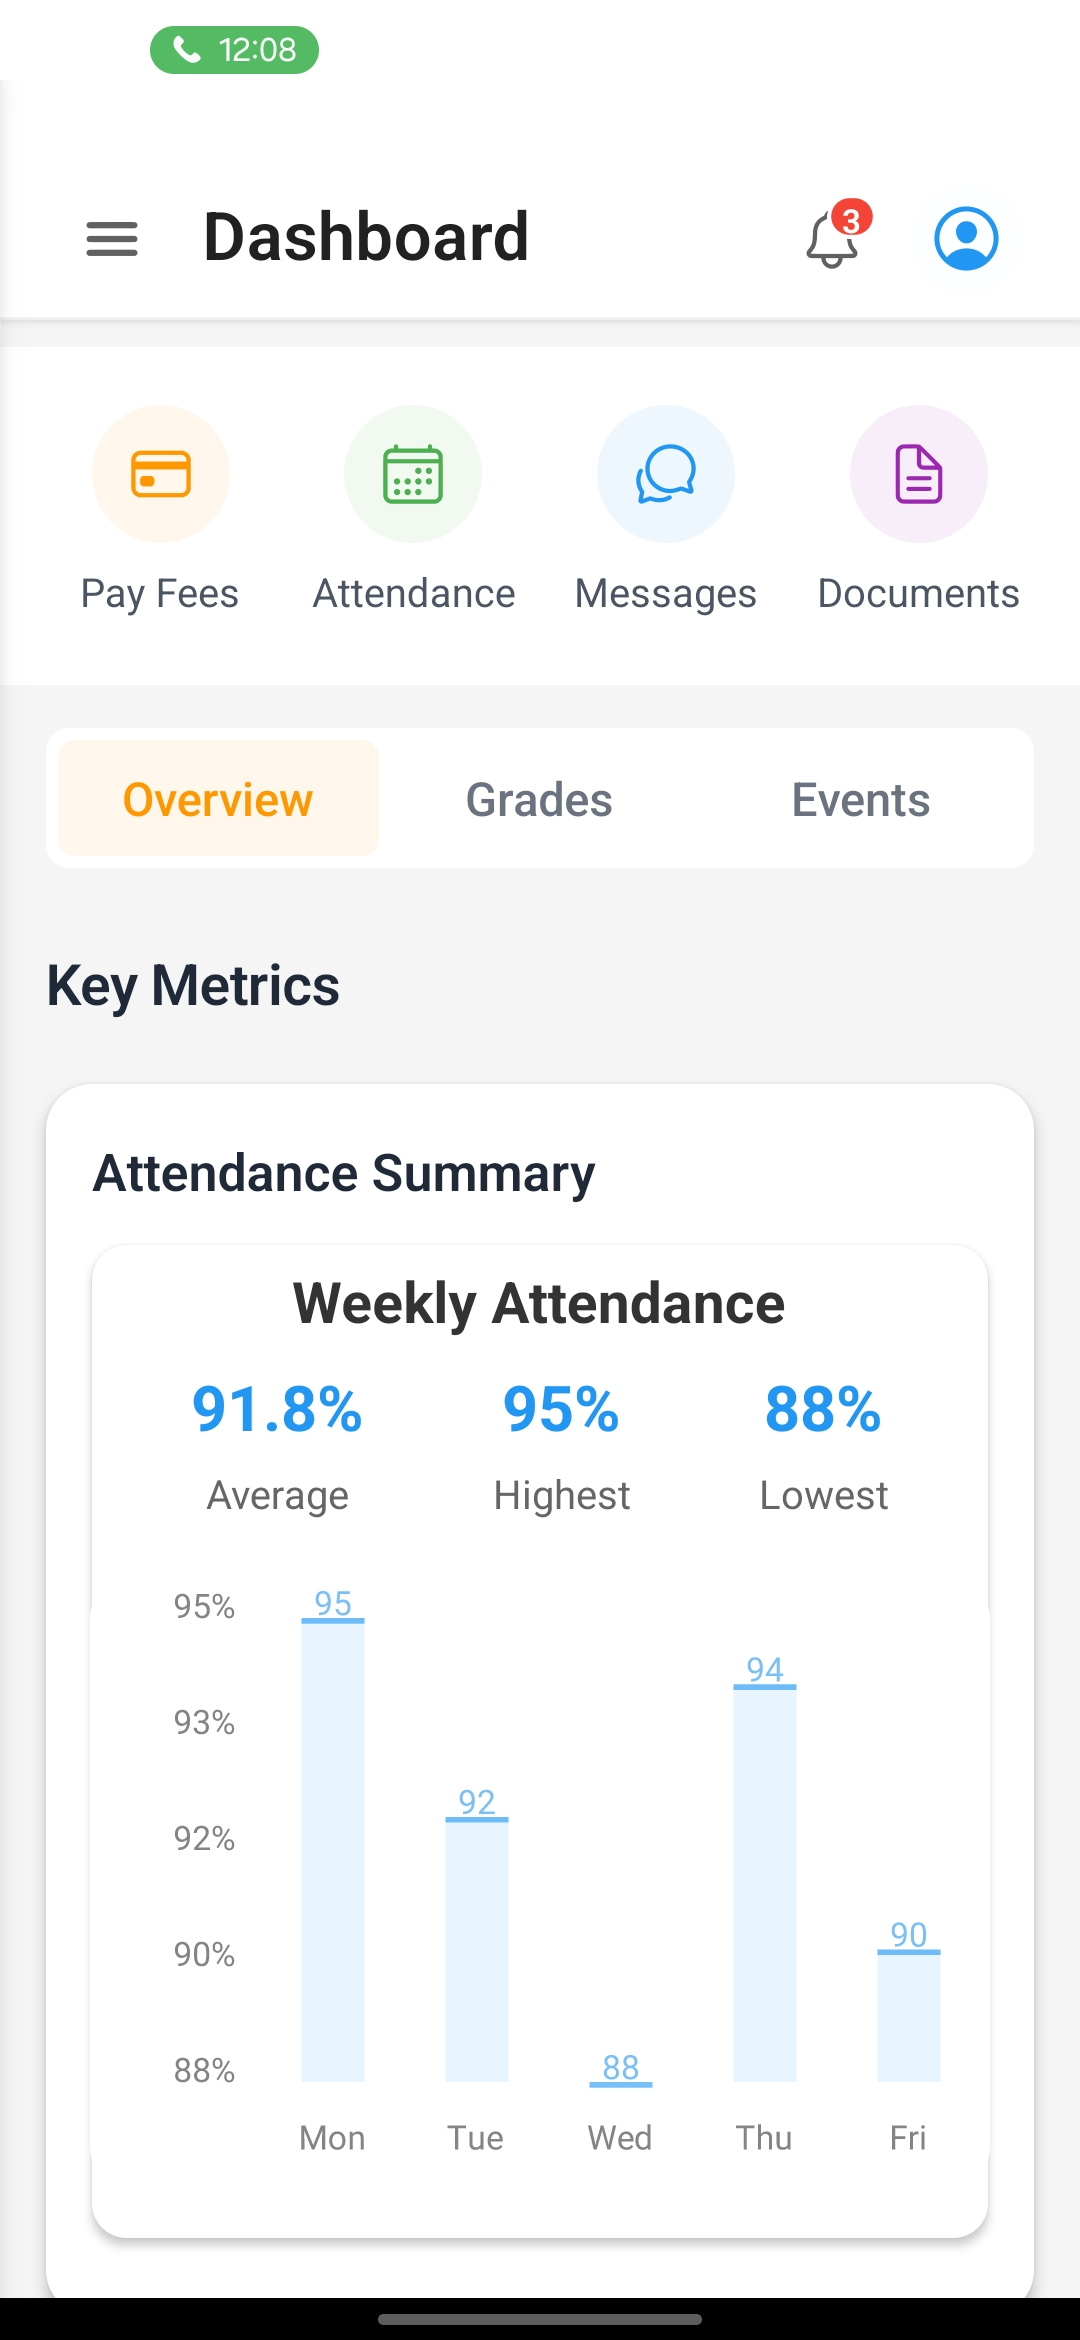
\includegraphics[width=0.4\textwidth,keepaspectratio]{pfe-pics/Mobile /Parent /Screenshot_20250610_132939_Expo Go.jpg}
  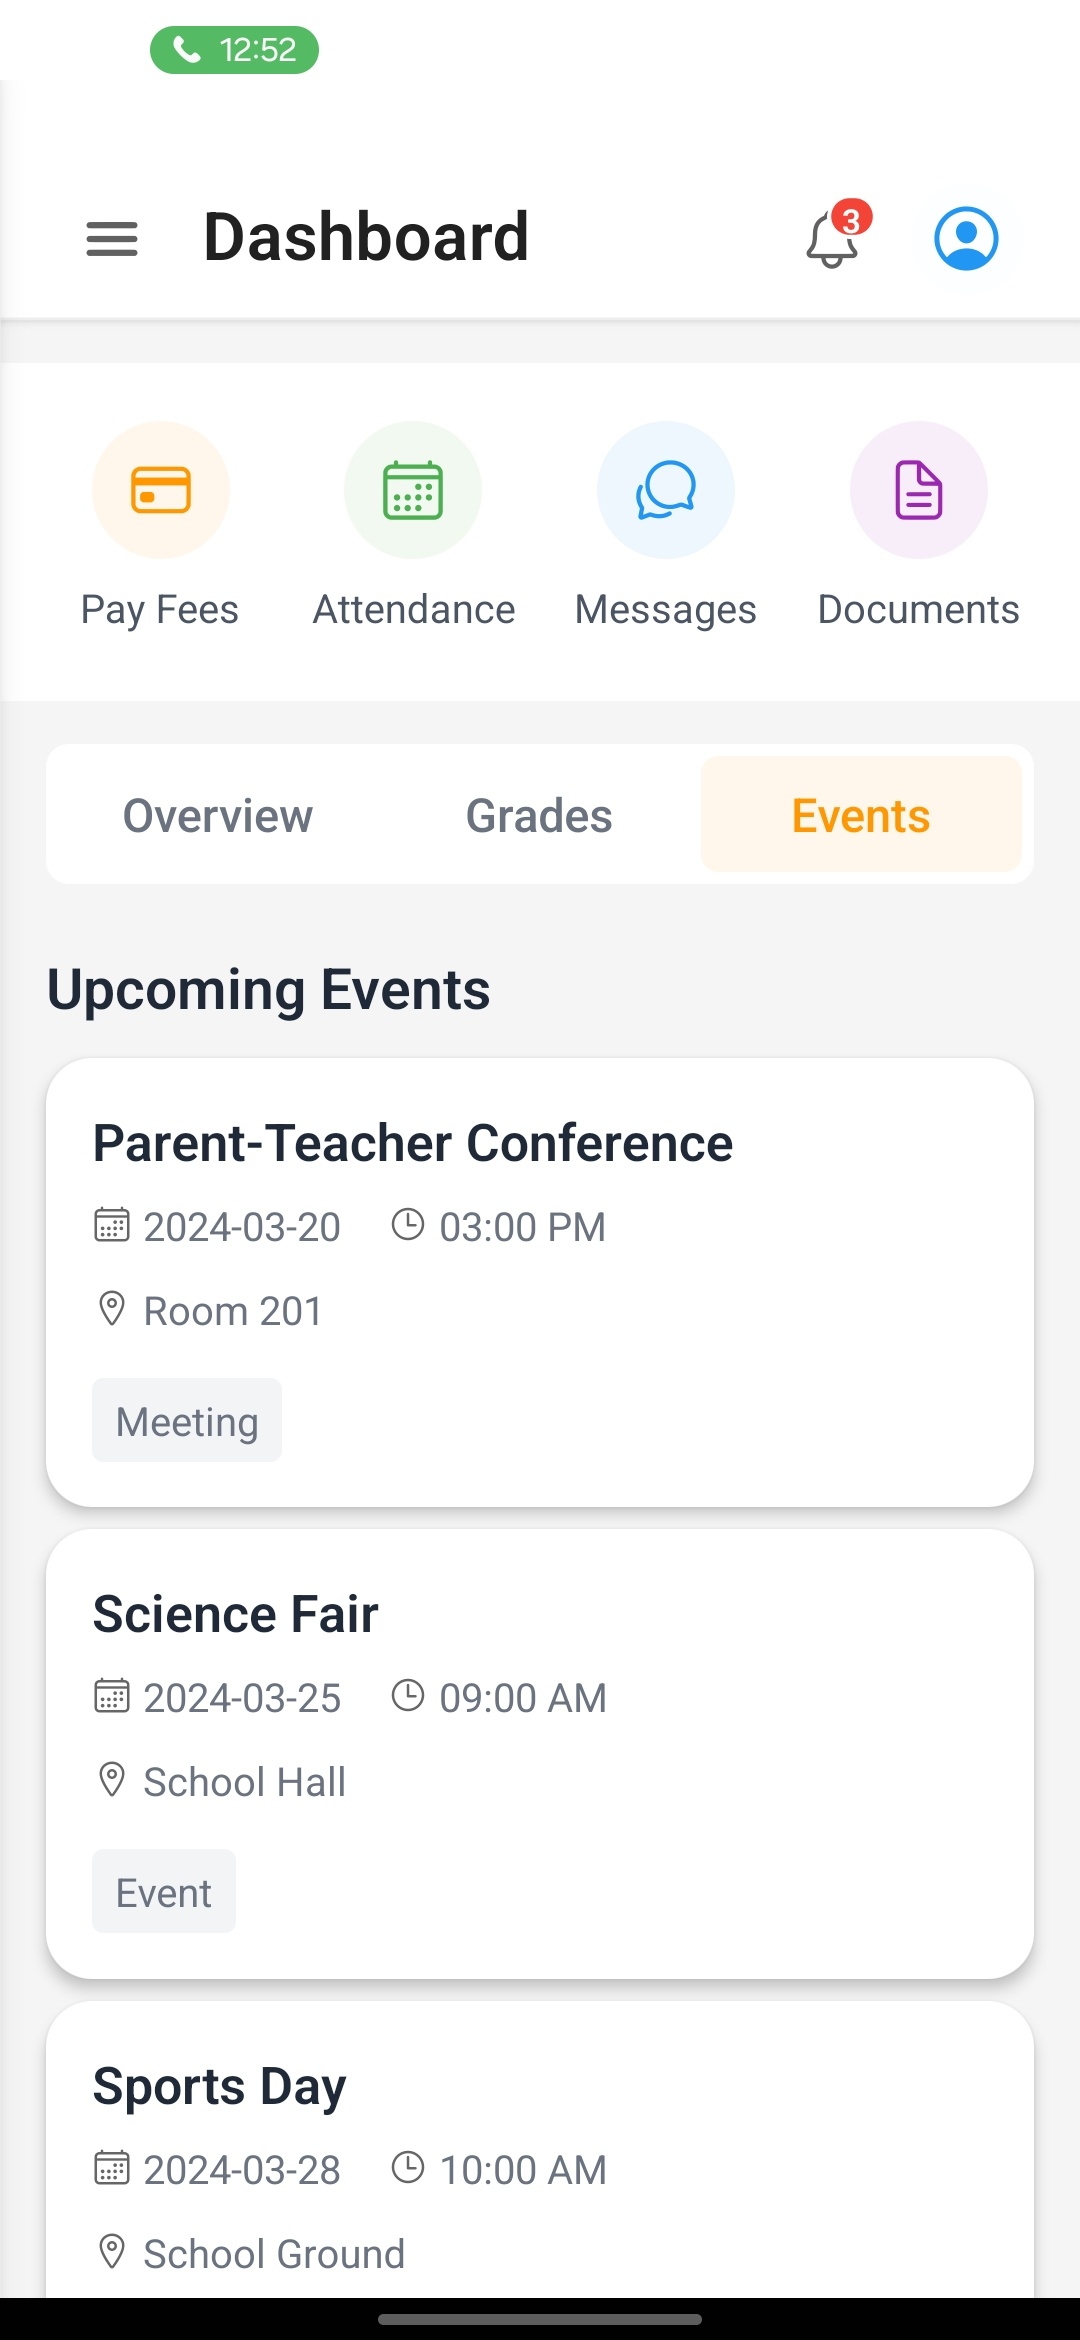
\includegraphics[width=0.4\textwidth,keepaspectratio]{pfe-pics/Mobile /Parent /Screenshot_20250610_133022_Expo Go.jpg}
  \caption{\textbf{Tableau de bord et sélection d'enfant} sur l'application mobile parent.}
  \label{fig:mobile_parent_dashboard}
\end{figure}

\begin{figure}[H]
  \centering
  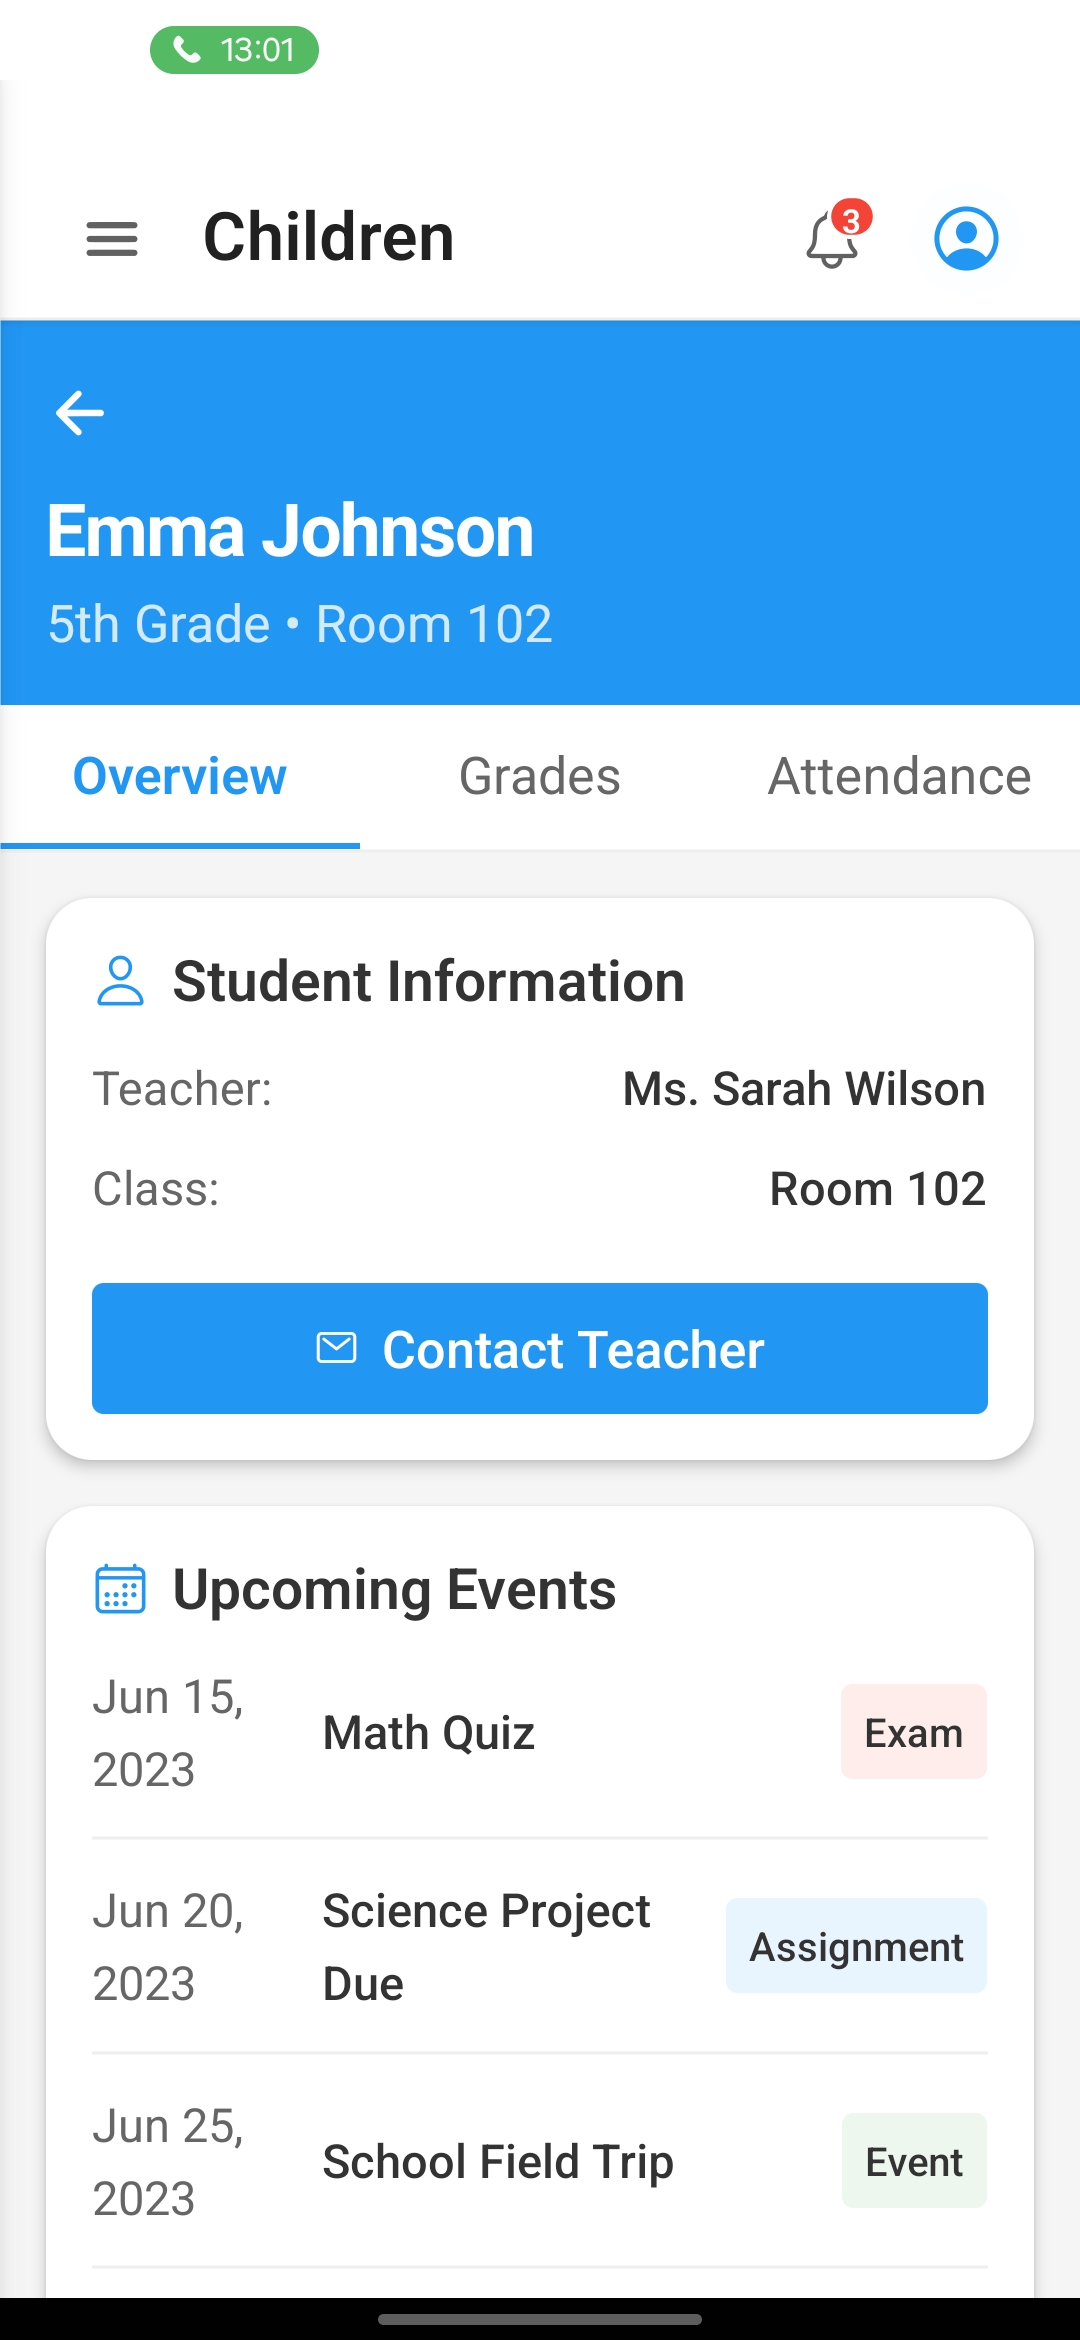
\includegraphics[width=0.4\textwidth,keepaspectratio]{pfe-pics/Mobile /Parent /Screenshot_20250610_133032_Expo Go.jpg}
  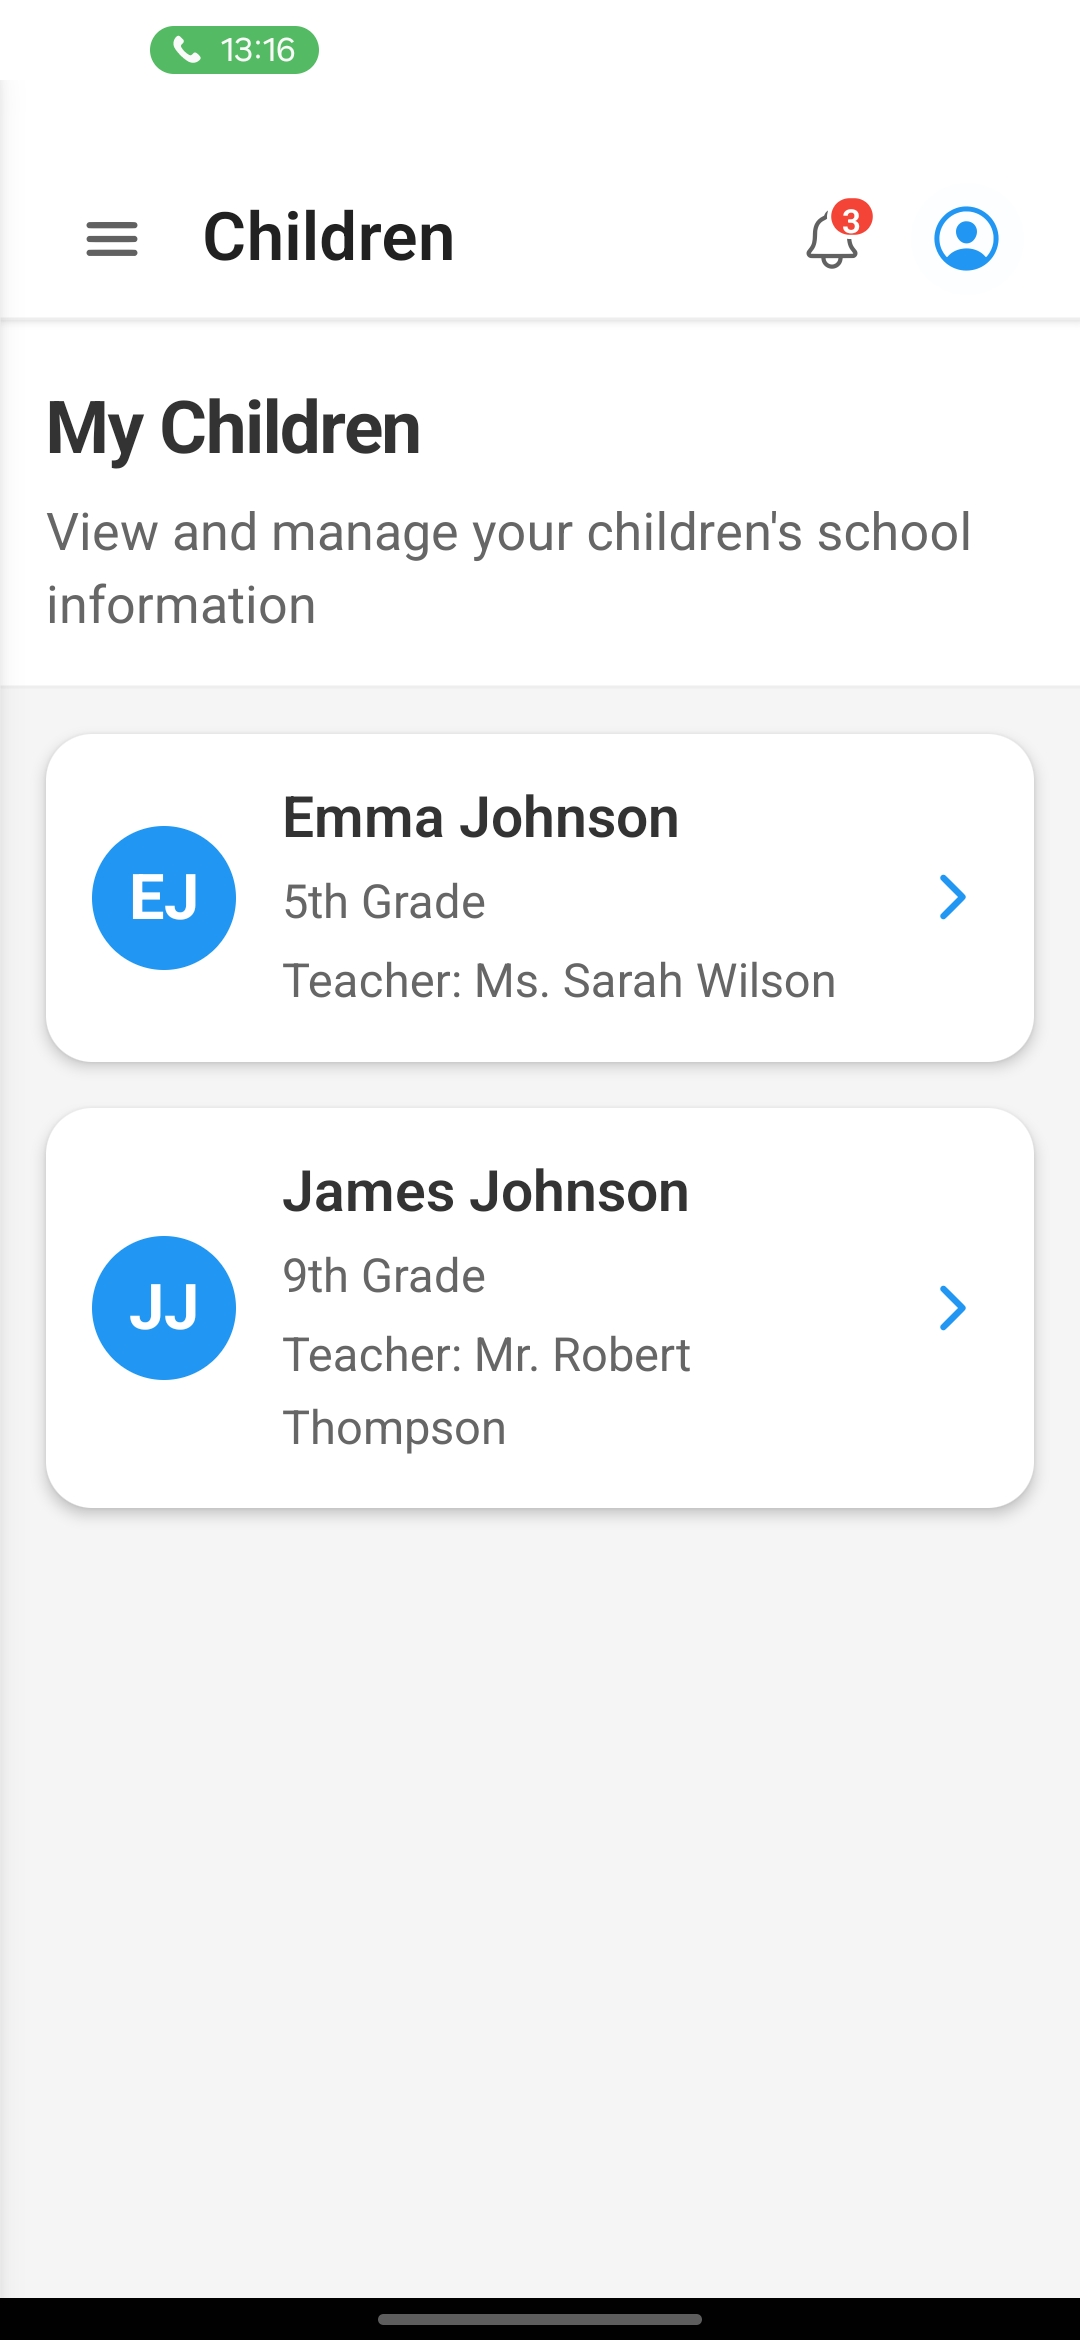
\includegraphics[width=0.4\textwidth,keepaspectratio]{pfe-pics/Mobile /Parent /Screenshot_20250610_133047_Expo Go.jpg}
  \caption{\textbf{Suivi des résultats et des présences} sur mobile pour les parents.}
  \label{fig:mobile_parent_monitoring}
\end{figure}

\subsubsection{Authentification mobile}

Le système d'authentification mobile offre une expérience sécurisée et conviviale :

\begin{figure}[H]
  \centering
  
\includegraphics[width=0.4\textwidth,keepaspectratio]{pfe-pics/Mobile /Auth/Screenshot_20250610_145348_Expo Go.jpg}
  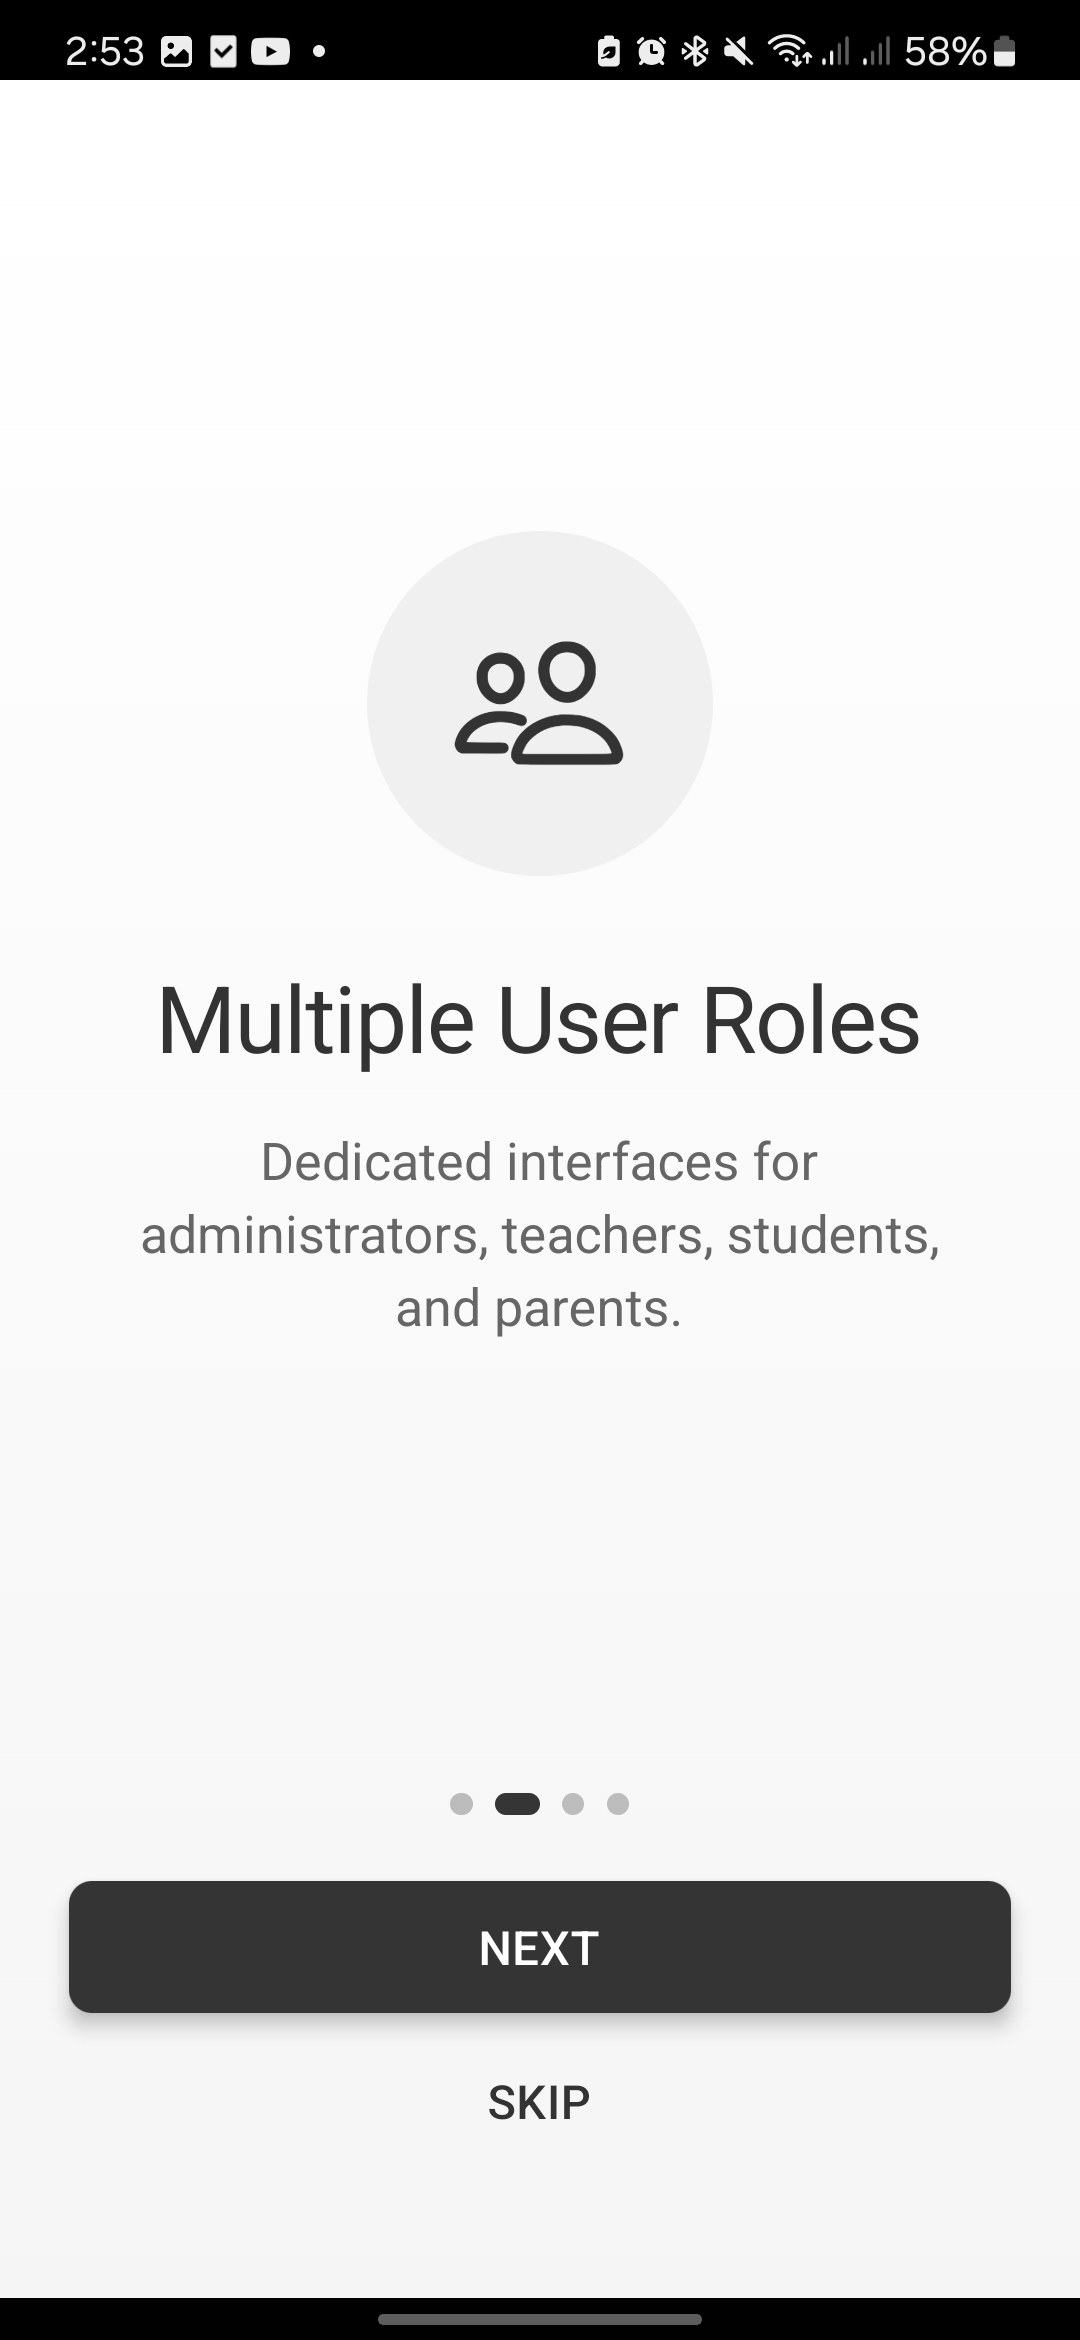
\includegraphics[width=0.4\textwidth,keepaspectratio]{pfe-pics/Mobile /Auth/Screenshot_20250610_145354_Expo Go.jpg}
  \caption{\textbf{Écrans de connexion et d'inscription} sur l'application mobile.}
  \label{fig:mobile_auth_screens}
\end{figure}

\section{Développement du système de création de profils IA}

Le développement du système de création de profils IA a représenté un défi technique particulier, combinant traitement de documents, intelligence artificielle et interfaces utilisateur intuitives.

\subsection{Implémentation du backend}

Le backend du système de création de profils IA a été développé avec FastAPI, un framework Python moderne offrant d'excellentes performances et une documentation automatique :

\begin{itemize}
  \item \textbf{Architecture API-first} : Conception d'une API RESTful complète comme fondation du système
  
  \item \textbf{Modèle de données} : Utilisation de Pydantic pour la validation et la sérialisation des données
  
  \item \textbf{Gestion asynchrone} : Implémentation d'opérations asynchrones pour optimiser les performances
  
  \item \textbf{Intégration avec OpenAI} : Connexion sécurisée avec l'API OpenAI via OpenRouter pour l'accès aux modèles de langage
  
  \item \textbf{Stockage hybride} : Combinaison de PostgreSQL pour les métadonnées et de stockage objet pour les documents
\end{itemize}

Voici un exemple de structure d'endpoint FastAPI pour la création d'un profil IA :

\begin{lstlisting}[style=codestyle, language=Python]
# app/routers/profiles.py
from fastapi import APIRouter, Depends, HTTPException, status
from sqlalchemy.ext.asyncio import AsyncSession
from typing import List

from app.schemas.profile import ProfileCreate, ProfileResponse
from app.services.profile_service import ProfileService
from app.dependencies import get_db, get_current_user
from app.models.user import User

router = APIRouter(prefix="/profiles", tags=["profiles"])

@router.post("/", response_model=ProfileResponse, status_code=status.HTTP_201_CREATED)
async def create_profile(
    profile_data: ProfileCreate,
    current_user: User = Depends(get_current_user),
    db: AsyncSession = Depends(get_db)
):
    profile_service = ProfileService(db)
    return await profile_service.create_profile(profile_data, current_user.id)

@router.get("/", response_model=List[ProfileResponse])
async def get_profiles(
    current_user: User = Depends(get_current_user),
    db: AsyncSession = Depends(get_db)
):
    profile_service = ProfileService(db)
    return await profile_service.get_user_profiles(current_user.id)
\end{lstlisting}

\subsection{Développement de l'interface utilisateur}

L'interface utilisateur du système de création de profils IA a été conçue pour être intuitive et efficace, permettant aux utilisateurs de créer et gérer facilement leurs profils IA :

\subsubsection{Page d'accueil et tableau de bord}

\begin{figure}[H]
  \centering
  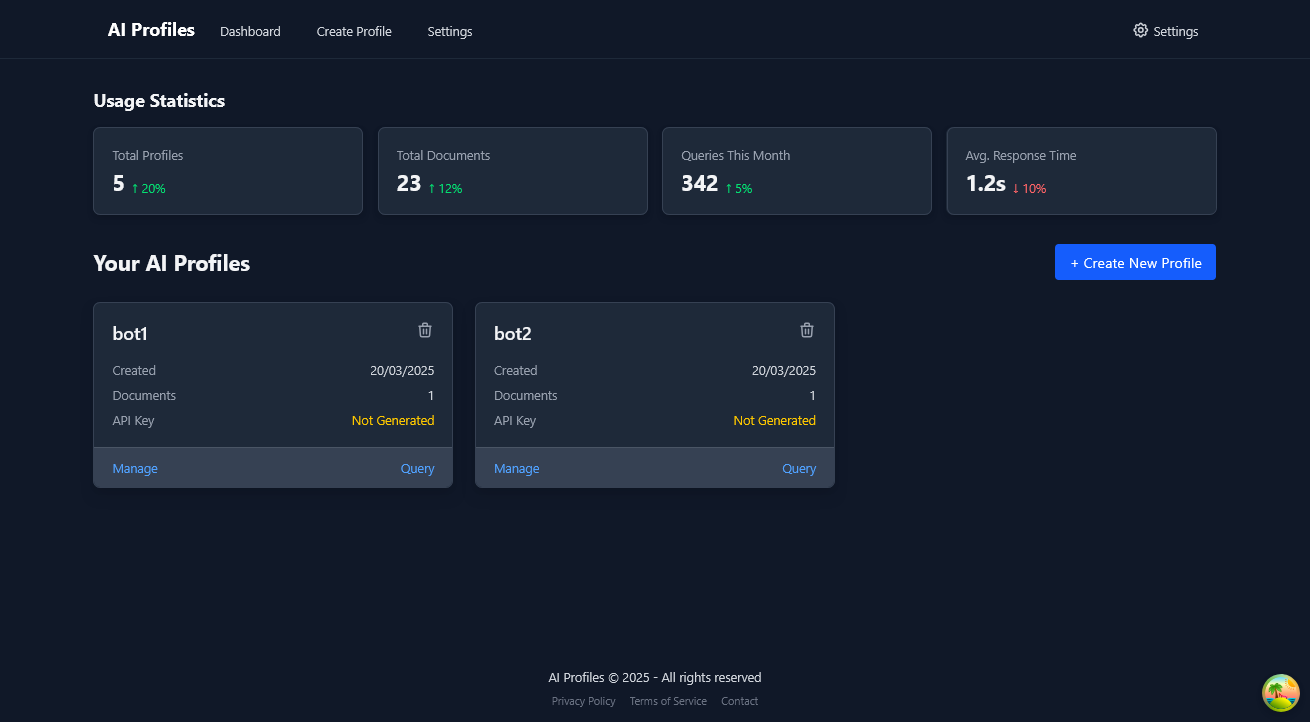
\includegraphics[width=0.85\textwidth,keepaspectratio]{pfe-pics/ai-profile-creation/dashboared_befor_adding_a_new_ai_profile.png}
  \caption{\textbf{Tableau de bord} du système de création de profils IA avant l'ajout d'un nouveau profil.}
  \label{fig:ai_dashboard}
\end{figure}

Le tableau de bord offre une vue d'ensemble des profils créés par l'utilisateur, avec des métriques clés comme :

\begin{itemize}
  \item Nombre de profils actifs
  \item Statistiques d'utilisation récente
  \item État de traitement des documents
  \item Accès rapide aux profils favoris
\end{itemize}

\subsubsection{Création et configuration de profil}

\begin{figure}[H]
  \centering
  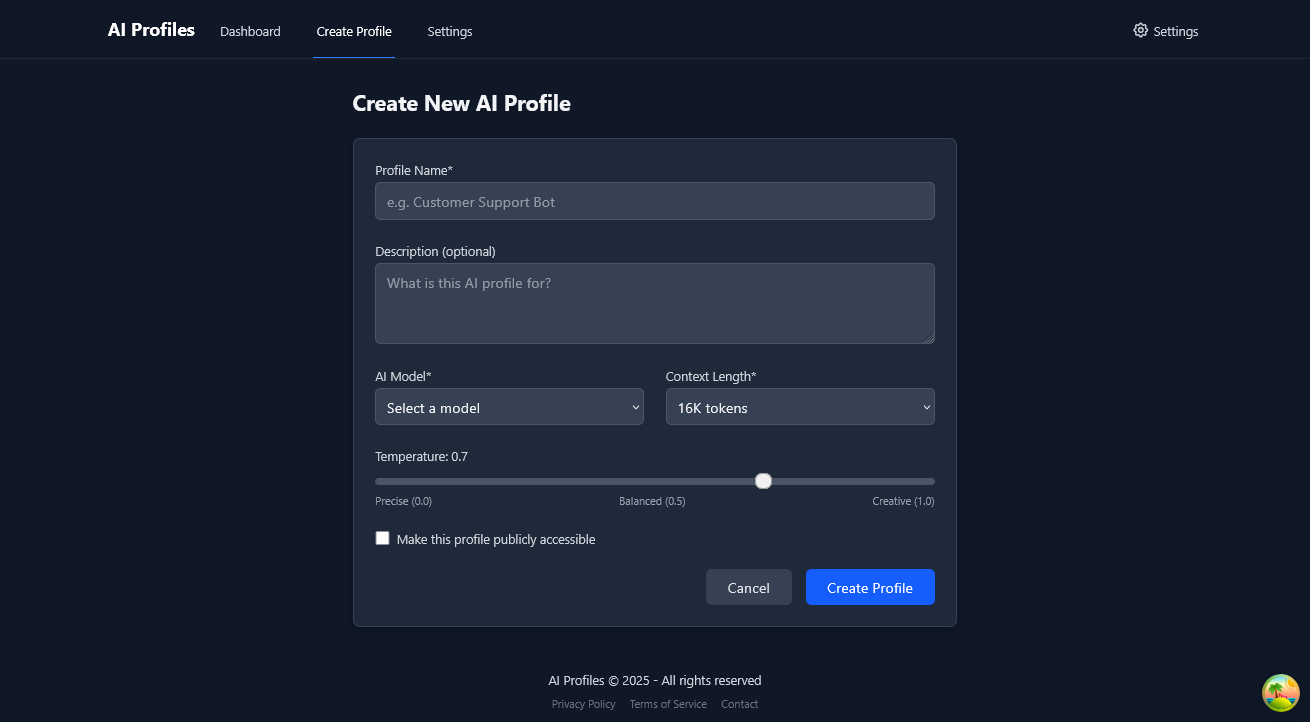
\includegraphics[width=0.85\textwidth,keepaspectratio]{pfe-pics/ai-profile-creation/creating_and_ai_prifile.png}
  \caption{\textbf{Interface de création de profil IA} avec options de configuration.}
  \label{fig:profile_creation}
\end{figure}

L'interface de création de profil permet aux utilisateurs de :

\begin{itemize}
  \item Définir les informations de base du profil (nom, description, domaine)
  \item Configurer le comportement de l'IA (ton, style de réponse, niveau de détail)
  \item Sélectionner des catégories et tags pour organiser les profils
  \item Définir les paramètres de confidentialité et d'accès
\end{itemize}

\subsubsection{Upload et gestion des documents}

\begin{figure}[H]
  \centering
  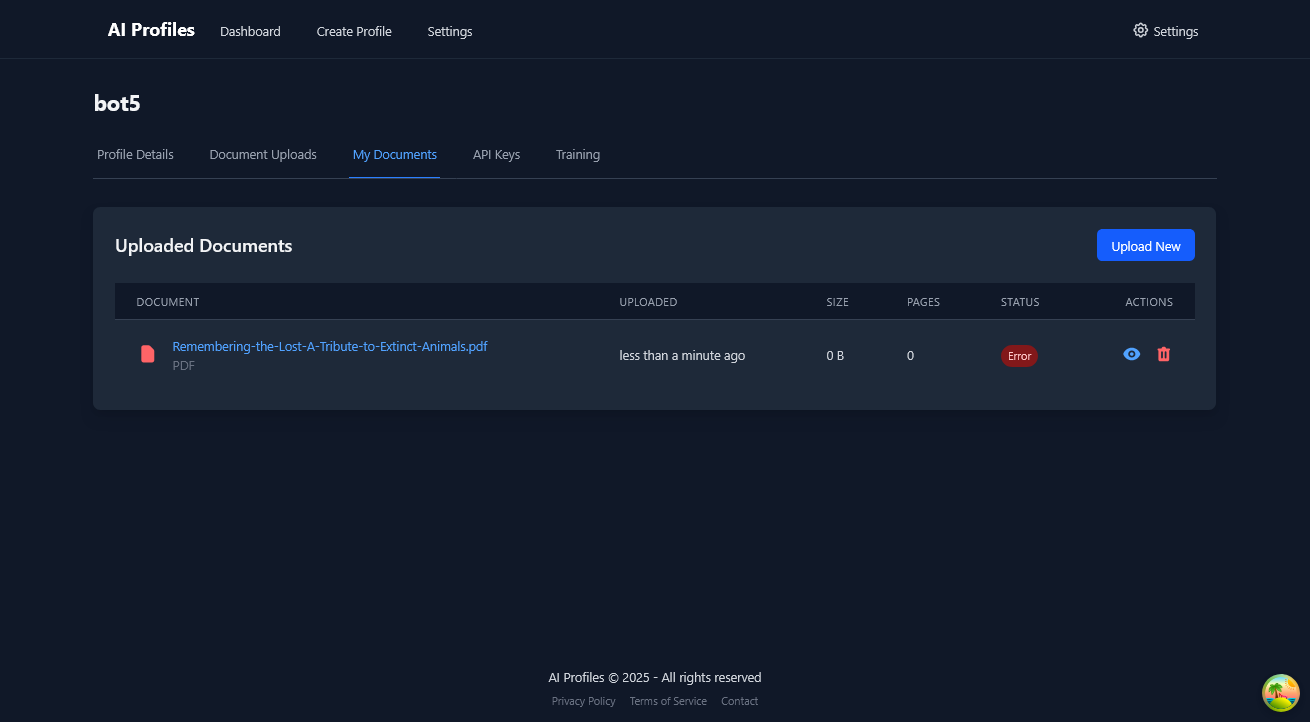
\includegraphics[width=0.85\textwidth,keepaspectratio]{pfe-pics/ai-profile-creation/see_upladed_documents_knoladge.png}
  \caption{\textbf{Interface de visualisation des documents uploadés} et leur connaissance associée.}
  \label{fig:document_knowledge}
\end{figure}

\begin{figure}[H]
  \centering
  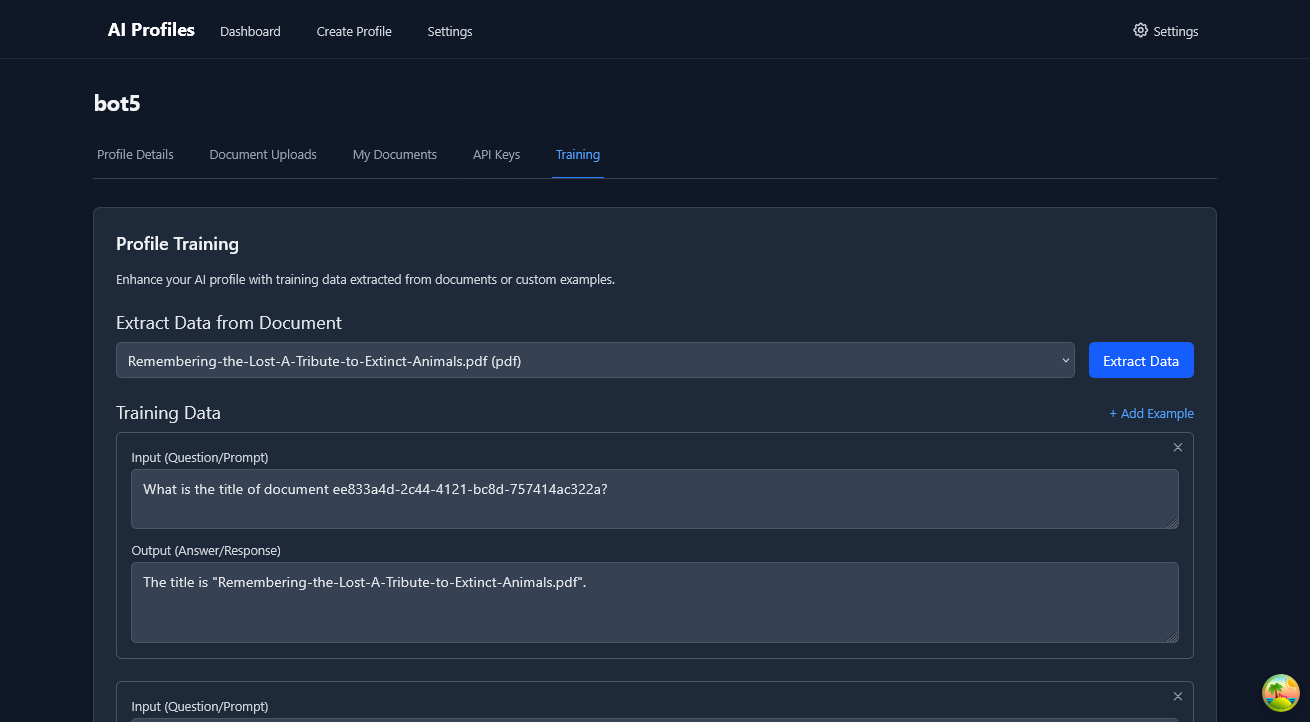
\includegraphics[width=0.85\textwidth,keepaspectratio]{pfe-pics/ai-profile-creation/extract_info_from_file_and_training_pfrile.png}
  \caption{\textbf{Interface d'extraction d'information} à partir des fichiers et entrainement du profil.}
  \label{fig:document_extraction}
\end{figure}

L'interface de gestion des documents offre des fonctionnalités avancées :

\begin{itemize}
  \item Upload par glisser-déposer de multiples formats (PDF, DOCX, TXT)
  \item Visualisation de l'état de traitement en temps réel
  \item Organisation des documents par catégories
  \item Prévisualisation du contenu extrait
  \item Possibilité d'ajouter des métadonnées et annotations
\end{itemize}

\begin{figure}[H]
  \centering
  \includegraphics[width=0.85\textwidth,keepaspectratio]{pfe-pics/ai-profile-creation/succesful_knoladge_integration.png}
  \caption{\textbf{Confirmation d'intégration réussie} des connaissances extraites dans le profil IA.}
  \label{fig:knowledge_integration}
\end{figure}

\subsubsection{Interface de test et conversation}

\begin{figure}[H]
  \centering
  \includegraphics[width=0.85\textwidth,keepaspectratio]{pfe-pics/ai-profile-creation/chat_interface_to_test_the_profile.png}
  \caption{\textbf{Interface de conversation pour tester le profil IA} créé.}
  \label{fig:profile_testing}
\end{figure}

\begin{figure}[H]
  \centering
  \includegraphics[width=0.85\textwidth,keepaspectratio]{pfe-pics/ai-profile-creation/chat_interface_for_testing_profile_2_test_prompt_succes.png}
  \caption{\textbf{Résultat réussi de test du profil} avec des prompts de vérification.}
  \label{fig:profile_test_success}
\end{figure}

L'interface de conversation permet une interaction naturelle avec les profils IA :

\begin{itemize}
  \item Design inspiré des applications de messagerie modernes
  \item Historique des conversations sauvegardé
  \item Affichage des sources documentaires pour les réponses
  \item Options de feedback pour améliorer les réponses
  \item Possibilité de partager des conversations
\end{itemize}

\subsubsection{Gestion des API et intégrations}

\begin{figure}[H]
  \centering
  \includegraphics[width=0.85\textwidth,keepaspectratio]{pfe-pics/ai-profile-creation/create_and_api_key_for_trained_profile.png}
  \caption{\textbf{Interface de création de clé API} pour un profil IA entrainé.}
  \label{fig:api_key_creation}
\end{figure}

\begin{figure}[H]
  \centering
  \includegraphics[width=0.85\textwidth,keepaspectratio]{pfe-pics/ai-profile-creation/adding_openRouter_api.png}
  \caption{\textbf{Interface d'ajout d'une clé API OpenRouter} pour l'accès aux modèles de langage.}
  \label{fig:openrouter_api_addition}
\end{figure}

\begin{figure}[H]
  \centering
  \includegraphics[width=0.85\textwidth,keepaspectratio]{pfe-pics/ai-profile-creation/oneRouter_keys_hestory.png}
  \caption{\textbf{Historique des clés API OpenRouter} utilisées par le système.}
  \label{fig:api_keys_history}
\end{figure}

Pour les utilisateurs souhaitant intégrer leurs profils IA dans d'autres applications :

\begin{itemize}
  \item Création et gestion de clés API avec permissions spécifiques
  \item Documentation interactive des endpoints disponibles
  \item Exemples de code pour différents langages de programmation
  \item Suivi de l'utilisation et des quotas
\end{itemize}

\begin{figure}[H]
  \centering
  \includegraphics[width=0.85\textwidth,keepaspectratio]{pfe-pics/ai-profile-creation/api_diagnostics.png}
  \caption{\textbf{Interface de diagnostics API} pour la vérification des problèmes d'intégration.}
  \label{fig:api_diagnostics}
\end{figure}

\begin{figure}[H]
  \centering
  \includegraphics[width=0.85\textwidth,keepaspectratio]{pfe-pics/ai-profile-creation/test_openRouter_connection.png}
  \caption{\textbf{Test de connexion OpenRouter} pour vérifier la configuration du service.}
  \label{fig:openrouter_test}
\end{figure}

\subsection{Pipeline de traitement des documents}

Le cœur du système de création de profils IA réside dans son pipeline de traitement des documents, qui transforme les documents bruts en base de connaissances structurée pour l'IA.

\subsubsection{Architecture du pipeline}

Le pipeline de traitement a été conçu comme un système asynchrone à plusieurs étapes :

\begin{itemize}
  \item \textbf{Réception et validation} : Vérification des formats et de l'intégrité des documents
  
  \item \textbf{Extraction de texte} : Conversion des différents formats en texte brut
  
  \item \textbf{Analyse structurelle} : Identification des sections, titres et éléments spéciaux
  
  \item \textbf{Segmentation intelligente} : Découpage en chunks optimisés pour la recherche sémantique
  
  \item \textbf{Génération d'embeddings} : Création de représentations vectorielles pour chaque segment
  
  \item \textbf{Indexation} : Stockage optimisé pour la recherche rapide
\end{itemize}

\subsubsection{Optimisation du chunking}

Une attention particulière a été portée à l'optimisation de la segmentation des documents :

\begin{itemize}
  \item \textbf{Chunking sémantique} : Découpage respectant la structure logique du contenu
  
  \item \textbf{Chevauchement contrôlé} : Inclusion partielle du contexte entre segments adjacents
  
  \item \textbf{Métadonnées enrichies} : Association de chaque segment à sa position et son contexte
  
  \item \textbf{Traitement spécifique} : Gestion adaptée des tableaux, listes et éléments spéciaux
\end{itemize}

\subsubsection{Intégration avec les modèles LLM}

L'interaction avec les modèles de langage a été optimisée pour obtenir les meilleures performances :

\begin{itemize}
  \item \textbf{Sélection contextuelle} : Identification des segments les plus pertinents pour chaque requête
  
  \item \textbf{Construction de prompts} : Génération dynamique de prompts optimisés incluant le contexte documentaire
  
  \item \textbf{Gestion du contexte conversationnel} : Maintien de la cohérence dans les échanges multi-tours
  
  \item \textbf{Mécanismes de fallback} : Stratégies alternatives en cas d'absence d'information pertinente
\end{itemize}

\section{Intégration et tests}

\subsection{Stratégie d'intégration}

L'intégration entre nos deux systèmes a été réalisée de manière progressive, en suivant une approche par étapes :

\begin{itemize}
  \item \textbf{Authentification unifiée} : Mise en place d'un système SSO permettant aux utilisateurs de naviguer entre les deux plateformes avec un seul compte
  
  \item \textbf{API Gateway commun} : Configuration de Nginx comme point d'entrée unifié pour les requêtes vers les deux systèmes
  
  \item \textbf{Partage de ressources} : Développement de mécanismes permettant l'utilisation des documents pédagogiques du système scolaire comme source pour les profils IA
  
  \item \textbf{Intégration UI} : Création de composants permettant d'accéder aux fonctionnalités des profils IA directement depuis l'interface du système scolaire
\end{itemize}

\subsection{Tests et validation}

Une stratégie de test complète a été mise en place pour garantir la qualité des deux systèmes :

\begin{itemize}
  \item \textbf{Tests unitaires} : Vérification du comportement isolé de chaque composant
  
  \item \textbf{Tests d'intégration} : Validation des interactions entre les différents modules
  
  \item \textbf{Tests end-to-end} : Simulation de scénarios utilisateur complets
  
  \item \textbf{Tests de performance} : Évaluation du comportement sous charge et optimisation
  
  \item \textbf{Tests d'utilisabilité} : Sessions avec des utilisateurs réels pour valider l'expérience utilisateur
\end{itemize}

\section{Déploiement et mise en production}

\subsection{Configuration de l'environnement de production}

La mise en production des systèmes a nécessité une configuration soignée de l'environnement :

\begin{itemize}
  \item \textbf{Infrastructure cloud} : Déploiement sur une infrastructure cloud flexible et évolutive
  
  \item \textbf{Conteneurisation} : Utilisation de Docker pour garantir la cohérence entre environnements
  
  \item \textbf{Équilibrage de charge} : Configuration de load balancers pour distribuer le trafic
  
  \item \textbf{Surveillance} : Mise en place d'outils de monitoring pour suivre la santé et les performances
  
  \item \textbf{Sauvegardes} : Stratégie de sauvegarde régulière des données critiques
\end{itemize}

\subsection{Stratégie de déploiement}

Une approche de déploiement continu a été adoptée pour minimiser les risques :

\begin{itemize}
  \item \textbf{Environnements multiples} : Séparation claire entre développement, test et production
  
  \item \textbf{Déploiement automatisé} : Utilisation de GitHub Actions pour l'intégration et le déploiement continus
  
  \item \textbf{Déploiement bleu-vert} : Stratégie permettant des mises à jour sans interruption de service
  
  \item \textbf{Rollback automatisé} : Mécanismes de retour arrière en cas de problème détecté
\end{itemize}

\section{Défis rencontrés et solutions apportées}

\subsection{Défis techniques}

Au cours du développement, plusieurs défis techniques significatifs ont été rencontrés :

\begin{itemize}
  \item \textbf{Traitement de documents hétérogènes} : La diversité des formats et structures de documents a complexifié l'extraction et l'analyse automatisées
  
  \item \textbf{Optimisation des requêtes LLM} : La construction de prompts efficaces pour obtenir des réponses précises et pertinentes a nécessité de nombreuses itérations
  
  \item \textbf{Performance des interfaces riches} : Le chargement et la manipulation de grandes quantités de données dans les interfaces utilisateur ont posé des défis de performance
  
  \item \textbf{Synchronisation mobile-web} : La cohérence des données entre les applications web et mobiles a nécessité une attention particulière
  
  \item \textbf{Sécurité des données sensibles} : La protection des informations personnelles et académiques a requis une approche de sécurité multicouche
\end{itemize}

\subsection{Solutions et optimisations}

Pour surmonter ces défis, plusieurs solutions innovantes ont été mises en œuvre :

\begin{itemize}
  \item \textbf{Pipeline de prétraitement modulaire} : Développement de modules spécialisés pour chaque type de document, avec des stratégies d'extraction adaptées
  
  \item \textbf{Optimisation des prompts par apprentissage} : Mise en place d'un système d'amélioration continue des prompts basé sur le feedback des utilisateurs
  
  \item \textbf{Stratégies de chargement différé} : Implémentation de techniques de virtualisation et pagination pour les interfaces manipulant de grandes quantités de données
  
  \item \textbf{Architecture offline-first} : Conception des applications mobiles avec synchronisation intelligente et fonctionnement hors ligne
  
  \item \textbf{Chiffrement de bout en bout} : Mise en œuvre du chiffrement pour les données sensibles, tant au repos qu'en transit
\end{itemize}

\section{Pages d'accueil et de présentation}

Les pages d'accueil et de présentation de nos systèmes ont été conçues pour être intuitives, informatives et visuellement attrayantes. Ces pages servent de point d'entrée pour les utilisateurs et présentent les principales fonctionnalités des plateformes.

\subsection{Page d'accueil du système de gestion scolaire}

\begin{figure}[H]
  \centering
  \includegraphics[width=0.85\textwidth,keepaspectratio]{pfe-pics/landing/hero.png}
  \caption{\textbf{Section d'accueil (Hero)} du système de gestion scolaire présentant l'offre principale.}
  \label{fig:landing_hero}
\end{figure}

\begin{figure}[H]
  \centering
  \includegraphics[width=0.85\textwidth,keepaspectratio]{pfe-pics/landing/info.png}
  \caption{\textbf{Section d'information} détaillant les caractéristiques clés de la plateforme.}
  \label{fig:landing_info}
\end{figure}

\begin{figure}[H]
  \centering
  \includegraphics[width=0.85\textwidth,keepaspectratio]{pfe-pics/landing/stats.png}
  \caption{\textbf{Section de statistiques} mettant en avant les résultats et l'impact du système.}
  \label{fig:landing_stats}
\end{figure}

\begin{figure}[H]
  \centering
  \includegraphics[width=0.85\textwidth,keepaspectratio]{pfe-pics/landing/Screenshot 2025-06-09 at 23-12-47 Vite React TS.png}
  \caption{\textbf{Section de tarification} présentant les différentes options d'abonnement.}
  \label{fig:landing_pricing}
\end{figure}

\begin{figure}[H]
  \centering
  \includegraphics[width=0.85\textwidth,keepaspectratio]{pfe-pics/landing/Screenshot 2025-06-09 at 23-12-17 Vite React TS.png}
  \caption{\textbf{Section des fonctionnalités} du système de gestion scolaire.}
  \label{fig:landing_features}
\end{figure}

\begin{figure}[H]
  \centering
  \includegraphics[width=0.85\textwidth,keepaspectratio]{pfe-pics/landing/contact.png}
  \caption{\textbf{Section de contact} avec formulaire permettant aux utilisateurs de demander des informations.}
  \label{fig:landing_contact}
\end{figure}

\begin{figure}[H]
  \centering
  \includegraphics[width=0.85\textwidth,keepaspectratio]{pfe-pics/landing/fotter.png}
  \caption{\textbf{Pied de page (Footer)} contenant les liens importants et informations légales.}
  \label{fig:landing_footer}
\end{figure}

\subsection{Pages de présentation du système de gestion scolaire}

Les composants de la page d'accueil et de présentation du système de gestion scolaire travaillent ensemble pour offrir une expérience utilisateur cohérente et informative, guidant les visiteurs depuis la découverte initiale jusqu'à la prise de contact ou l'inscription.

\section{Environnement de développement personnel}

Pour le développement de ces deux systèmes complémentaires, un environnement de développement personnel optimisé a été configuré, permettant une productivité maximale et une expérience de développement fluide.

\subsection{Système d'exploitation et outils principaux}

\begin{itemize}
  \item \textbf{Système d'exploitation} : Arch Linux, choisi pour sa flexibilité, sa légèreté et sa capacité de personnalisation avancée
  
  \item \textbf{Éditeur de code principal} : Neovim avec une configuration personnalisée incluant des plugins pour le développement web, Python et TypeScript
  
  \item \textbf{Éditeur secondaire} : VSCodium (version open-source de VS Code), utilisé principalement pour le débogage et les fonctionnalités d'édition collaboratives
  
  \item \textbf{Terminal} : Alacritty avec configuration tmux pour la gestion efficace des sessions multiples
  
  \item \textbf{Shell} : Zsh avec le framework Oh My Zsh et des plugins pour Git, Docker et Node.js
\end{itemize}

\subsection{Environnement de base de données}

\begin{itemize}
  \item \textbf{MySQL} : Utilisé comme système de gestion de base de données relationnelle principal pour le système de gestion scolaire
  
  \item \textbf{XAMPP} : Suite de développement local intégrant Apache, MariaDB et PHP pour le développement rapide
  
  \item \textbf{PostgreSQL} : Utilisé pour le système de création de profils IA
  
  \item \textbf{MongoDB} : Utilisé pour certaines fonctionnalités spécifiques nécessitant une structure de données plus flexible
  
  \item \textbf{Redis} : Utilisé pour la mise en cache et la gestion des sessions
\end{itemize}

\subsection{Outils de développement frontend}

\begin{itemize}
  \item \textbf{Node.js} et \textbf{npm} : Pour la gestion des dépendances et l'exécution des scripts
  
  \item \textbf{Vite} : Comme outil de build rapide pour le développement frontend
  
  \item \textbf{React Developer Tools} : Pour le débogage des composants React
  
  \item \textbf{TypeScript} : Pour un développement typé et plus robuste
  
  \item \textbf{ESLint} et \textbf{Prettier} : Pour le linting et le formatage automatique du code
\end{itemize}

\subsection{Outils de développement backend}

\begin{itemize}
  \item \textbf{Postman} : Pour tester et documenter les API
  
  \item \textbf{Python avec pyenv} : Pour la gestion de plusieurs versions de Python
  
  \item \textbf{Docker} et \textbf{Docker Compose} : Pour la conteneurisation des services
  
  \item \textbf{Swagger UI} : Pour la documentation interactive des API
\end{itemize}

\section{Glossaire des abréviations}

\begin{itemize}
  \item \textbf{API} : Application Programming Interface - Interface de programmation d'application permettant la communication entre différents logiciels
  
  \item \textbf{CSS} : Cascading Style Sheets - Langage de feuille de style utilisé pour décrire la présentation d'un document écrit en HTML
  
  \item \textbf{CRUD} : Create, Read, Update, Delete - Opérations de base pour la persistance des données
  
  \item \textbf{DOM} : Document Object Model - Interface de programmation pour les documents HTML et XML
  
  \item \textbf{IA} : Intelligence Artificielle - Ensemble des théories et techniques développant des programmes informatiques complexes capables de simuler certains traits de l'intelligence humaine
  
  \item \textbf{JWT} : JSON Web Token - Standard ouvert basé sur JSON pour créer des jetons d'accès
  
  \item \textbf{LLM} : Large Language Model - Modèle de langage de grande taille utilisé pour générer et comprendre le langage naturel
  
  \item \textbf{ORM} : Object-Relational Mapping - Technique de programmation informatique qui crée une couche d'abstraction entre la base de données relationnelle et le modèle objet
  
  \item \textbf{REST} : Representational State Transfer - Style d'architecture pour les systèmes distribués
  
  \item \textbf{SSO} : Single Sign-On - Méthode permettant à un utilisateur d'accéder à plusieurs applications avec un seul identifiant
  
  \item \textbf{UI} : User Interface - Interface utilisateur, partie visible d'une application avec laquelle interagit l'utilisateur
  
  \item \textbf{UX} : User Experience - Expérience utilisateur, ensemble des interactions et expériences vécues par l'utilisateur
  
  \item \textbf{WSGI} : Web Server Gateway Interface - Spécification simple et universelle pour l'interface entre les serveurs web et les applications web pour Python
  
  \item \textbf{XAMPP} : Cross-Platform (X), Apache, MariaDB, PHP, Perl - Suite logicielle constituant un environnement de développement web
\end{itemize}


% --- Conclusion ---
\chapter*{Conclusion et Perspectives}
\addcontentsline{toc}{chapter}{Conclusion et Perspectives}
\thispagestyle{fancy}
\setcounter{section}{0}
\newpage

Ce projet de fin d'études a permis de développer deux systèmes complémentaires qui répondent aux besoins actuels des établissements éducatifs : un système de gestion scolaire complet et une plateforme innovante de création de profils IA.

\section{Bilan du projet}

Le développement de ces deux systèmes a abouti à des solutions fonctionnelles et robustes :

\begin{itemize}
  \item \textbf{Système de gestion scolaire} : Une application multiplateforme offrant des interfaces adaptées à chaque type d'utilisateur (administrateur, enseignant, étudiant, parent), avec des fonctionnalités complètes pour la gestion des cours, des présences, des évaluations et de la communication.
  
  \item \textbf{Plateforme de création de profils IA} : Un système permettant de transformer des documents en assistants virtuels intelligents, avec un pipeline de traitement sophistiqué et une interface utilisateur intuitive.
  
  \item \textbf{Intégration} : Des mécanismes d'intégration entre les deux systèmes, permettant d'enrichir l'expérience éducative en combinant gestion administrative et assistance intelligente.
\end{itemize}

L'approche architecturale adoptée, basée sur des principes modernes comme la modularité, la séparation des préoccupations et la scalabilité, a permis de créer des systèmes évolutifs et maintenables.

\section{Compétences acquises}

Ce projet a été l'occasion de mettre en pratique et d'approfondir de nombreuses compétences :

\begin{itemize}
  \item \textbf{Développement web et mobile} : Maîtrise de React, Node.js, FastAPI, React Native et des technologies associées
  
  \item \textbf{Architecture logicielle} : Conception d'architectures multicouches et microservices
  
  \item \textbf{Intelligence artificielle} : Intégration de modèles de langage et traitement automatique de documents
  
  \item \textbf{Gestion de projet} : Organisation du travail, respect des délais et documentation
  
  \item \textbf{Sécurité et performance} : Implémentation de bonnes pratiques pour des applications robustes et performantes
\end{itemize}

\section{Perspectives d'évolution}

Les systèmes développés offrent de nombreuses perspectives d'évolution :

\begin{itemize}
  \item \textbf{Architecture microservices complète} : Migration progressive vers une architecture entièrement basée sur les microservices pour améliorer la scalabilité et la résilience des systèmes
  
  \item \textbf{Intégration de bases de données vectorielles} : Utilisation de bases de données vectorielles pour optimiser le stockage et la recherche des embeddings dans la plateforme de création de profils IA
  
  \item \textbf{Amélioration de l'intelligence artificielle} : Intégration de modèles plus avancés et personnalisation accrue des réponses
  
  \item \textbf{Fonctionnalités analytiques} : Développement d'outils d'analyse des données éducatives pour identifier des tendances et optimiser l'apprentissage
  
  \item \textbf{Intégration plus poussée} : Renforcement des synergies entre le système de gestion et la plateforme IA
  
  \item \textbf{Internationalisation} : Adaptation des systèmes pour différentes langues et contextes éducatifs
  
  \item \textbf{Accessibilité} : Amélioration de la conformité aux standards d'accessibilité pour une inclusion plus large
\end{itemize}

\section{Mot de fin}

Ce projet de fin d'études a constitué une expérience enrichissante, tant sur le plan technique que personnel. Il m'a permis de confronter mes connaissances théoriques à des problématiques concrètes et de développer des solutions innovantes dans le domaine éducatif.

Les défis rencontrés, notamment dans le traitement des documents et l'optimisation des performances, ont été autant d'opportunités d'apprentissage et de dépassement. La satisfaction de voir les systèmes fonctionner et répondre aux besoins identifiés est une récompense précieuse pour les efforts investis.

Je suis convaincu que les compétences et l'expérience acquises durant ce projet constitueront des atouts majeurs pour ma future carrière professionnelle dans le domaine du développement logiciel.

% --- Bibliography ---
\chapter*{Bibliographie}
\addcontentsline{toc}{chapter}{Bibliographie}
\thispagestyle{fancy}
\setcounter{section}{0}

\begin{itemize}
  \item React Documentation, \url{https://reactjs.org/docs}
  
  \item Node.js Documentation, \url{https://nodejs.org/en/docs}
  
  \item FastAPI Documentation, \url{https://fastapi.tiangolo.com/}
  
  \item React Native Documentation, \url{https://reactnative.dev/docs}
  
  \item Expo Documentation, \url{https://docs.expo.dev/}
  
  \item Tailwind CSS Documentation, \url{https://tailwindcss.com/docs}
  
  \item MongoDB Documentation, \url{https://docs.mongodb.com/}
  
  \item PostgreSQL Documentation, \url{https://www.postgresql.org/docs/}
  
  \item OpenAI API Documentation, \url{https://platform.openai.com/docs/}
  
  \item Docker Documentation, \url{https://docs.docker.com/}
  
  \item MySQL Documentation, \url{https://dev.mysql.com/doc/}
  
  \item ArchWiki, \url{https://wiki.archlinux.org/}
  
  \item Mermaid Diagramming and Charting Tool, \url{https://mermaid.js.org/}
  
  \item JWT (JSON Web Tokens), \url{https://jwt.io/}

  \item Express.js Documentation, \url{https://expressjs.com/}
  
  \item ESLint Documentation, \url{https://eslint.org/docs/latest/}
  
  \item Git Documentation, \url{https://git-scm.com/doc}
\end{itemize}

\end{document} 